\documentclass[
    paper=letter,
    parskip=half,
    fontsize=12pt,
    titlepage=firstiscover,
    toc=bibliography,
    numbers=endperiod
]{scrartcl}
\usepackage[utf8]{inputenc}
\usepackage{amssymb}   % Additional symbols
\usepackage{csquotes}  % Context-sensitive quotes
\usepackage[backend=biber,style=ieee]{biblatex}
\usepackage{booktabs}  % Convenience shortcuts for tables
\usepackage{etoolbox}  % Adds additional hooks like \AtBeginEnvironment
\usepackage{fancyvrb}  % Fancy verbatim environments
\usepackage{float}     % Enables exact-placement of figures
\usepackage{geometry}  % Sets page margins
\usepackage{graphicx}  % Set additional properties (like dimensions) to graphics
\usepackage[hidelinks]{hyperref} % Enables linking
\usepackage[none]{hyphenat} % Disable hyphenation
\usepackage{newtxtext} % Adds Times New Roman
\usepackage{setspace}  % Sets line spacing
\usepackage{soul}      % Better handling of certain text styles
\usepackage{tabularx}  % Adds automatically-sized tables
\usepackage{ltablex}   % Extension of tabularx for extending over pages
\usepackage{url}       % Better display of URLs in references
\usepackage{xpatch}    % Extension of etoolbox

\addbibresource{references.bib}
\graphicspath{ {./images/} }

% Add the command \tightlist
\providecommand{\tightlist}{%
  \setlength{\itemsep}{0pt}\setlength{\parskip}{0pt}}

% Define a blockquote
\AtBeginEnvironment{quote}{\par\singlespacing\small}

% Add resizable centered and left-aligned table columns
\newcolumntype{C}{>{\centering\arraybackslash}X}
\newcolumntype{L}{>{\raggedright\arraybackslash}X}

% From setspace package
\setstretch{1.2}

% 1 inch margins
\AfterCalculatingTypearea{\geometry{margin=1in}}
\recalctypearea

% New page after sections
\let\oldsection\section
\renewcommand{\section}{\newpage\oldsection}

% Center all images
\makeatletter
\g@addto@macro\@floatboxreset\centering
\makeatother

% Show 4 levels of depth in TOC
\setcounter{secnumdepth}{\paragraphtocdepth}
\setcounter{tocdepth}{\paragraphtocdepth}

% Use Times New Roman
\addtokomafont{disposition}{\rmfamily}

\title{SWIM}
\subtitle{Simple Web Interface for MIPS}
\author{
    Kevin Cahalan
    \and
    Jerrett Longworth
    \and
    Huy Nguyen
    \and
    Evan Raiford
    \and
    Jimmie Smith
}

% TODO: With the exception of the personal sections, ALL text should be written in we/our/us voice.

\begin{document}

\sloppy

\maketitle

\pagenumbering{arabic}
\setcounter{page}{1}
\tableofcontents

\section{Executive Summary}

SWIM (Simple Web Interface for MIPS) is a web interface to view and
interact with a MIPS64 emulator, designed by Kevin Cahalan, Jerrett
Longworth, Huy Nguyen, Evan Raiford, and Jimmie Smith. This project was
initially pitched by Kevin Cahalan and was designed in Senior Design at
the University of Central Florida in Fall 2022.

SWIM is intended to contain a self-contained package of everything
needed to write programs in assembly, assemble them to binary
instructions for MIPS64, execute the instructions in a simulated
processor of the same architecture, and to visualize the execution of
this processor. The purpose of this project is intended to supplement
computer architecture courses, with a specific focus on the instruction
set architecture used in the curricula at the University of Central
Florida, MIPS. Regardless of the skill level and knowledge of students
who use this software, SWIM ultimately serves to assist students in
furthering their understanding of computer architecture.

SWIM's design offers additional flexibility compared to other emulators,
being designed in a way that could easily allow for future development
and features, as well as having open support for alternative instruction
set architectures. This serves the dual purpose of SWIM to not only be
an educational tool for students in an isolated environment, but to last
as a solution that can continue to be used in the future, regardless of
what instruction set architectures later become prominent.

% TODO: Licensing
SWIM is planned to be available to use by anyone at no cost. Similarly,
SWIM will be licensed under the GNU General Public License to allow
anyone to freely view the project's code and modify it as seen fit for
the free distribution to others.

Subsequent sections of this document outline and organize the design
process for SWIM, including research into the MIPS64 instruction set
architecture, project requirements and specifications, and project code
management. The following section describes in more detail the
motivations and outline of the project, and later sections describe its
successes, challenges, and auxiliary information surrounding its design.

\section{Overview}

\subsection{Project Description}
\label{subsec:project-description}

When studying Computer Science or a related field, students must learn
about computer architecture and design, which includes assembly
languages and instruction set architectures. In many universities,
including the University of Central Florida, the chosen instruction set
architecture is MIPS32. If students proceed to take more advanced
courses centered on computer architecture, they inevitably encounter
MIPS64 in that process, as well.

While there are already a number of emulators and tools available for
students and instructors to learn and teach MIPS, there can be a number
of issues surrounding them that make them difficult or even impossible
to use in some cases. Current options for MIPS emulation software are
overly-complex or use out-of-date frameworks. Our project aims to be a
new, alternative MIPS emulation tool that is easier to digest compared
to existing options. The current go-to option for educational MIPS
simulation is SPIM \cite{spim}. While it has a rich feature-set, SPIM is
no longer actively maintained, is aging since its original release in
1990, and is not user-friendly by modern standards.

Additionally, most other MIPS emulation options \cite{wepsim, jsspim,
    wemips, mips-interpreter, mini-mips, mips-assembler-field-guide,
    mips-assembler-hogan, cpulator}, including SPIM, only support MIPS32,
meaning the 64-bit extension of MIPS, MIPS64, is unsupported. Many
students do not attempt to use SPIM unless required by their courses due
to these limitations. Due to this, learning low-level programming
concepts, a task that is already difficult in and of itself, is even
more difficult for most students than it needs to be. The goal of SWIM
is to change this outcome, where students should be interested and want
to use the emulator to study for classes and self-taught individuals
should be able to use it to satisfy curiosity. Both groups of people
should experience a minimal learning curve when it comes to interacting
with the MIPS pipeline. SWIM aims to become the standard for MIPS
education as a standard emulator for both MIPS32 and MIPS64.

Our solution to this issue is SWIM, a simple web interface for MIPS32
and MIPS64. SWIM is a MIPS emulator that supports a subset of both
MIPS32 and MIPS64, and completely runs within a web browser. In SWIM,
people can write and run MIPS32 and MIPS64 programs in browsers with an
enhanced text editor with line-by-line execution, view register and
memory contents, and recognize MIPS pseudo-instructions in a modern,
easy-to-use interface. Making an emulator that supports both major
versions of MIPS means that students will be able to use SWIM throughout
an extended part of their low-level programming education, especially
considering alternative options for MIPS emulation. Being browser-based,
the barrier for entry is much lower than downloaded software, is
agnostic to any one platform or operating system, and accessible from
anywhere with an internet connection. Having modern features like
step-through debugging and register viewing will make the development
experience more similar to modern languages and easier to work with.

The code for the project is written primarily in Rust \cite{rust-book}
to utilize its secure memory management systems, type checking, and
borrow checking. Where necessary, JavaScript and TypeScript is used to
supplement this for web-based development. The text editing interface
uses the Monaco library \cite{monaco} due to its existing familiarity
with programmers. The server-side component of SWIM merely serves to
deliver content and application files. SWIM implements a strong subset
of the instructions supported by MIPS32 and MIPS64.

\subsubsection{The Tech Stack}
SWIM's tech stack is unique in the fact that a lot of the tools and
frameworks used in its development are still in their preliminary
stages, unlike conventional tools such as JavaScript, React, Emscripten,
and MongoDB. This project's tech stack uses the Rust programming
language for developing all parts of the application: emulation core,
parser, and interface. This helps with having a cohesive understanding
of how the codebase is structured, as all code from all components use
the same programming language.

Moving up to abstraction in Rust, the Yew framework \cite{yew} and Gloo
toolkit \cite{gloo} facilitates how the front end interacts with
Javascript APIs and aids in converting Rust code into the appropriate
WebAssembly binaries and JavaScript files without direct intervention or
understanding from a development perspective. WebAssembly
\cite{webassembly} is still in its infancy, but it allows our Rust code
to be run on browsers like Google Chrome, Mozilla Firefox, Apple Safari,
and Microsoft Edge. Due to the recency of WebAssembly, users must run
the latest version of those browsers – or their respective FOSS forks
(i.e. Chromium, Waterfox, etc.) – in order for WebAssembly to function
properly. While the majority of code running for this project is in
WebAssembly, JavaScript is still essential for the application to
initially load on the web browser. Trunk \cite{trunk} is the tool for
packaging and finalizing the software; Trunk has configurations that
allows us to automatically re-compile the software as we edit it.

GitHub Pages is used to host SWIM, additionally allowing users access to
the project's source code on the same site. For the user interface,
Microsoft's Monaco Editor is used, given its support for assembly
syntax, Intellisense, themes, and its extensible API.

\begin{figure}[H]
    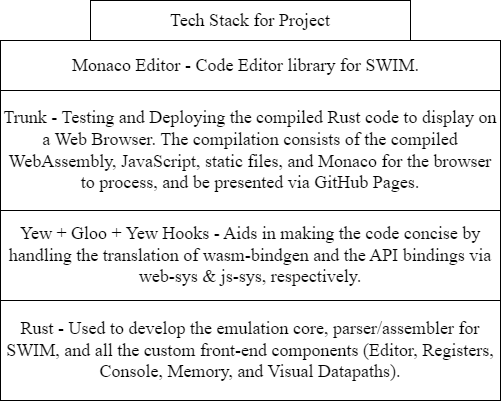
\includegraphics[height=10cm]{tech-stack}
    \caption{Visualization of the Tech Stack}
\end{figure}

\subsection{Project Motivation}

The motivation behind SWIM, at its root, is at the major flaws in the
currently-available resources in the educational MIPS emulation scene.
As mentioned in Section \ref{subsec:project-description}, there are no
real options for those who want to learn MIPS64. In addition, most if
not all existing options for MIPS32 emulation arguably have an
unnecessary learning curve to being used. Many students in computer
architecture courses dread learning and using MIPS, as there is simply
not the same level of assistance available that many students have
become accustomed to expect. For example, if a student wants to learn
Python, there is a plenitude of resources to help them along the way.
There are countless Python IDEs, online resources for running Python,
and so forth. For learning MIPS, most of the information found will be
from a textbook or course lectures, and many members of the project team
have been directly affected by this environment.

In addition, a major motivation of any software development project is
to accomplish something amazing; something that we felt was realistic
and useful. Much of the team is comprised of low-level programming
enthusiasts, making the mission of the project even more plausible and
usable in real-world scenarios than the perspective of a traditional
programmer. Along the way, we want to improve our own understanding of
computation and computer architecture by building a core component of a
computer processor. Writing a MIPS emulator an interesting project, and
best of all, has clear direction. From the initial project pitch, it is
understood how the project will generally work and what it can do.

Many of the initial project proposals in Senior Design seemed to have no
real-world use or clear direction, coming from individuals with little
technical experience. The time and difficulty for some projects were
underestimated from a technical perspective, and some only generically
indicate what problem it solves or what purpose it has. Artificial
intelligence and virtual/augmented reality have been cited as catch-all
solutions to many problems, which is contrary to the beliefs of the
project team. While it can be very hard to gauge the difficulty and time
needed for a project without clear direction, we do not have the time or
luxury to gamble on a project to get lost on. This MIPS emulation
project felt like a great balance between direction and difficulty.

% TODO: Source of demand
Currently there is a significant demand in industry for custom
emulation. To become a professional emulator developer, small steps of
learning are required. By writing this emulator, our team is taking a
small step in this direction and we provide a better understanding of
emulator development. The ability to understand all parts of a computing
system -- RAM, flash memory, register states, and so on -- are crucial
to working with emulation. Additionally, physical hardware can be
limited based its interfaces, may be costly to develop on, or in some
cases inaccessible altogether. Security researchers want to be able to
create as many virtual environments as possible with minimal cost to
understand everything a system does.

\subsection{Individual Motivations}
\subsubsection{Kevin Cahalan}
\begin{figure}[H]
    
\includegraphics[height=7cm]{profile-kevin}
\end{figure}

For a while I have been wanting to write an awesome emulator. Things
kept getting in the way, I never got to it. Ever since I first started
learning Python, I have had an urge to get the ultimate understanding of
computers. Python sucked, it did not feel like programming. Writing
Python felt like telling a program what to do, not a computer. There was
clearly magic underneath. I hated having these magical devices out there
that I could simply not fathom or imagine. Computers seemed to be true
magic. To go further down my journey of getting a true understanding of
computers, I started learning C. C was a breath of free air. The more I
programmed in C, the more computers made sense. Writing my first
emulator, some emulator for a computer from the 70s, I took a big step
in learning the magic behind computing. Emulation development turns out
to be a great way for clearing away the magic property of computers.
When writing an emulator, you are effectively writing your own computer
in software. By working on SWIM I will be continuing my journey to get
the ultimate understanding of computation. I will further fight the
mysterious magic of computation.

Another big individual motivation for this are the job prospects. There
is solid money out there for emulation development. Emulators have all
sorts of uses, hacking, training, testing, legacy hardware replacement,
and so on. In the world of professional hacking, the need for automation
fits hand in hand with emulator development. Automated bug finders need
a surface to play with. Preferably a scalable surface. Using real
hardware can get super expensive very fast. It can be millions or
billions of dollars, sometimes impossible to get. With training it is
not best to trust a new person with expensive equipment. Issues of money
and safety come into play. It would not be the best idea to just drop
someone into an f-35, you start them with an accurate flight simulator.
So accurate that you emulate the computers within the aircraft for the
simulation. When testing new software for an f-35, initially using a
real aircraft would be unsafe. You test your software in emulation. In
the world of banking there are old legacy computers that need to be
replaced. Re-writing the software for these ancient computers can be
very risky and costly. The solution is to write an emulation layer to
port so that the old software could run on modern computers. With many
more examples out there, emulation happens to be very important for this
world. And the best part of all this, there's big money in the industry.

\subsubsection{Jerrett Longworth}
\begin{figure}[H]
    
\includegraphics[height=7cm]{profile-jerrett}
\end{figure}

From first being introduced to computer architecture and processor logic
and design at UCF, I was immediately interested in the subject area and
wanted to learn more. This topic, along with similar low-level topics
such as assembly languages, became a focus of mine throughout my
Computer Science studies. In the popular open-world sandbox game
Minecraft, I designed logic and built circuitry from scratch for a
system that takes a binary number and displays it on an in-game
seven-segment display. While studying Computer Logic and Organization
(CDA 3103) with Sarah Angell, I had already begun to think about the
utility and overall interest factor of having a live graphical
representation of a CPU performing instructions in its pipeline, not
only for an Instruction Set Architecture like MIPS, but for x86 and ARM
as well. SWIM offers this first step into creating a visualization such
as this.

I have thought about various forms, both in hardware and software, that
could achieve this effect. Inspired by an engineering sample of an
Nvidia 30-series graphics card, a hardware approach could have a
dedicated pin on the processor that reports some basic information like
the current instruction opcode or instruction pointer. A software
approach could be a graphical overlay over a high-definition image of
the internals of a CPU. A user could be given a live view of the bits
changing as a virtual CPU executes instructions, and you could pan and
zoom around the parts of the processor to see values located in
registers, memory, and other components.

Based on these ideas, I feel SWIM is an incredibly valuable project,
both for the educational factor for classes like CDA 3103, but also for
the personal enjoyment and satisfaction of watching this piece of
technology run at its most exposed state.

Another reason why this project is important to me is due to my
affiliation with Wiki Knights, which is a student organization dedicated
to reducing or eliminating the costs of textbooks and homework access
codes by encouraging the adoption of Open Educational Resources (OER) in
courses across the university. This group has already been developing a
free Introduction to C Programming (COP 3223) textbook with examples and
practice problems, which is currently deployed in classes as of the time
of writing. Further development is active within the group to re-open
the Adaptive Learning Engine project authored by the ALOSI Labs as a
collaboration between Harvard University's Office of the Vice Provost
for Advances in Learning and Microsoft. Along these efforts, an
open-source project such as SWIM offers another free resource for
students, course instructors, and researchers in areas related to
computer architecture.

\subsubsection{Jimmie Smith}
\begin{figure}[H]
    
\includegraphics[height=7cm]{profile-jimmie}
\end{figure}

While I pitched a project for this class with a similar topic, I figured
this was a more noble project to do. As someone who enjoyed CDA3103 and
EEL4768, SWIM could be the first step to educating people who are
interested in Assembly in a friendlier environment. Funnily enough, my
pitch has the same underlying goal as SWIM of modernizing the “old”
workflow with enhancements and visual feedback that makes it easier for
the user to understand the concept and have fun with it, too. Recently,
I have been learning about the Motorola 68000 since it was a CPU that
was used extensively back then, so I have a general feel for CISC and
RISC assembly with their concepts. I also have an affinity for emulation
since it is fun to explore older systems, and you can preserve, study,
and make new tools for them.

This is my first time being relegated to front-end development solely so
it is a huge responsibility to make sure the whole suite is presented in
an appropriate manner. Even though I have been assigned to work on the
front end with Rust, I am excited to understand Rust since I heard
people giving praise for its design compared to C. I have a few ideas of
my own on how I want the program to look since user experience is key.
Learning Assembly is hard to sell compared to high-level languages,
there are not that many good online tutorials for assembly, it is much
more verbose, and it has a steeper learning curve so interactivity is my
top-priority. This is a nice challenge for me since I have to constantly
ask myself how to make SWIM fun to use while the back end focuses on
creating a good emulation core.

My experience with MIPS in the past was easy-going at first, but by the
time I took Computer Architecture it became overwhelming especially when
it came to the different datapaths. By the end of the course, I was
having a difficult time understanding the concepts and how significant
they are. I had a harder time finding any tools that would help me
understand MIPS64 compared to MIPS32, so SWIM would fill in that gap.
With SWIM, it would not only remedy any confusions with MIPS64's
concepts but it can also be the basis for studying different types of
architecture and their feature set.

\subsubsection{Evan Raiford}
\begin{figure}[H]
    
\includegraphics[height=7cm]{profile-evan}
\end{figure}

My motivation for this project stems from multiple different places. The
first reason is that I see a need for the existence of a tool such as
this. One of the restricted electives I chose to take was EEL4768,
Computer Architecture, and a large part of that class was understanding
the changes necessary to implement a 64-bit system as opposed to a
32-bit system and the language used to detail these changes was MIPS64.
Examples drawn out on the board and thorough explanations are great
tools to assist in learning but for many people, myself included, the
best way to get a grasp on things is to try them out themselves. Having
a version of MIPS64 readily accessible would be a great tool to help
students learn.

A second, albeit related, reason I am motivated for this project is that
I am hopeful that we can build a tool that makes MIPS more approachable
for students. One of my absolute favorite things about my experience
earning my computer science degree has been building a solid
understanding of how a computer works from the bottom up. Assembly
languages, such as MIPS, are one of the foundational aspects of this.
However, assembly languages can often come across as intimidating and
hard to approach for new learners so students frequently only learn
enough to get through their class. I think a solid understanding of
basic instruction set architectures is vital to being a well-rounded
software developer. My hope is that the SWIM project will help make MIPS
and low-level programming concepts more approachable for the average
student.

The idea of making SWIM browser based is another reason I am motivated
for this project. Making it browser-based makes the software more
approachable for students since they would not need to download anything
onto their devices to use it. It also means it is more readily
accessible for instructors. If an instructor wants to use software that
has to be downloaded in a lecture hall, they often do not have the
option to download the software onto whatever device is used in the
lecture hall so they, instead, have to bring their own device with them
and hook that up to the projector in order to use the software in a
lecture. Having SWIM online circumvents that issue entirely. If somebody
wanted to use SWIM in a lecture, the software is accessible through the
browser so all they would need to do is navigate to the website.

Another reason that I am motivated for this project is the lack of a
sponsor. Having a sponsor on a project does give a lot of benefits like
financial backing, industry experience and advice, and a guiding hand.
However, they often also come with their own motivations for the
project, often hoping to use the tool to help bolster their business.
Doing a project without a bespoke sponsor ensures that whatever we make
is not beholden to somebody else's vision of what it can or should be.
Doing it without a sponsor also ensures that our end product is one made
wholly by us. Any issues we have along the way, we ourselves are the
ones that overcome them. The project that we make is one that we are
able to make solely on the experience that we have gained ourselves
either on our own or at UCF.

\subsubsection{Huy Nguyen}
\begin{figure}[H]
    
\includegraphics[height=7cm]{profile-huy}
\end{figure}

My motivation for the project stems from my experience with some of the
materials needed for this project, about the MIPS pipeline. The idea of
an accessible web-based MIPS emulation would have helped me and my peers
a lot back when I was studying Computer Architecture and System
Softwares. It would also make these subjects a lot easier on students
who need to take those, as well as being interested to learn more about
MIPS, which in turn would help with easier and more understandable
teaching than what me and my peers went through during those classes in
the past.

I am also attracted to this project by the prospect of not needing a
sponsor. Not having a sponsor means a few things. One of those things is
that we as a group are not constrained by the sponsors' demands, which
means we can be more comfortable in giving project ideas so that it
looks like what the group thinks it is, not what anyone outside thinks
it is. This would also mean anything we need to spend on for the project
we have to spend ourselves, and we also have to set deadlines ourselves,
which may be hard or distracting. However, I believe this will get me
more familiar with these kinds of projects where the idea is from a
single person and it is up to me and my group to expand on, not just a
pre-laid road by a company. Although I may lose the experience of
working with a sponsor, I currently have an opportunity to make a
project that I may be able to talk about in the future, which is this
project. This project would also hopefully improve my skills working
with my teammates, as it will undoubtedly help with further group
projects and careers in general in the future.

This project also seems like an opportunity to come in contact with more
variety in coding, as the project currently aims to run mostly on the
front end in Rust, a language I have never touched before. After having
a look at it, it seems solid, so it made me look forward to using it on
a project and adding one more language to my arsenal. That will also
mean I get to learn more about web development, specifically running an
emulator online, and what it entails.

\subsection{Group Member Ideas}
At the project's initial inception and gathering of group members, all
group members contributed ideas to brainstorm the features and
capabilities that would be supported by the project. Some of these ideas
have been implemented into the project or its stretch goals, and others
are left as possible suggestions for future revisions of the project.
The following are the ideas provided by each group member.

\subsubsection{Kevin Calahan}
\begin{itemize}
    \item The project itself.
    \item The use of Rust for programming both the back end and front end.
    \item Test driven development. All instructions should have test cases to
          prove that they work correctly.
    \item Naming the project “OurSPIM.” This name was based on an assignment named
          “MySPIM.” We decided that we do not want our own SPIM.
          % TODO: Unclear sentence
    \item The possible project name “MipAndNayNay64.” This project name is based
          off the song “Watch Me.”
    \item That way at which our instruction decode code would be written.
    \item How instructions are going to be handled in our codebase.
\end{itemize}

\subsubsection{Jerrett Longworth}
\begin{itemize}
    \item Interactive live view of the emulator pipeline with access to memory and
          register contents. A user could hover over various components or traces
          with their mouse to see their current contents.
    \item Alternative live view of the pipeline, which is overlaid onto a
          real-world image of a CPU die. This could be zoomed or panned to see
          individual bits in any of the components.
    \item Ability to view and change memory and register contents during
          execution.
    \item Communication to and from the user with a virtual display and input,
          communicated through an emulated bus.
    \item A “tutorial/educator mode,” which would allow an educator to create
          overlays and control the interface automatically to guide students to
          learn about a specific concept.
    \item A “quiz mode,” which would allow an educator to create overlays similar
          to the “tutorial mode,” but with interactive questions and problems that
          can report results to an LMS such as Instructure Canvas.
\end{itemize}

\subsubsection{Jimmie Smith}
\begin{itemize}
    \item As a design goal, SWIM should not only support MIPS64 but it should be
          designed openly to load in different emulators of CPUs and their
          respective datapaths (if available). This would require some careful
          planning, but should be feasible since this is being built from scratch.
    \item Having a live debugger for SWIM would be a simple feature to implement,
          but could streamline the debugging process even more.
    \item Since this is a web application, I think having customizable options
          would elevate the user experience like dark mode, color-coding for
          instructions, registers, etc.
\end{itemize}

\subsubsection{Evan Raiford}
\begin{itemize}
    \item An account system so that users are able to store something that they
          have been working on and then come back and continue working on it
          later. This would also allow lecturers the opportunity to store work
          that they can then access in a lecture.
    \item A tool that explains the function of instructions.
    \item Prefabricated programs that users can take a look at and mess around
          with to get a feel for how things are done in MIPS. A brief overview and
          explanation of what is being done and why could accompany it.
    \item The name that we ended up going with: SWIM. A Simple Web Interface for
          MIPS.
\end{itemize}

\subsubsection{Huy Nguyen}
\begin{itemize}
    \item We can make the front end look more accessible by giving the MIPS
          pipeline map more space as well as making the UI fit viewing mode, or
          hide them.
    \item Testing on Eustis3. Although I do think that this may not work or take
          forever to load the front end since our project is front end heavy.
    \item Admin accounts for testing front ends and account creations if
          necessary.
\end{itemize}

\subsection {Individual Roles}
Due to the highly technical nature of this project, it would have been
difficult for everybody on the team to work equally in each of the
different types of work required for making SWIM. Because of this, we
had each member of the team focus on a specific discipline and only help
out on other parts of the project when necessary. Listed below are the
individual roles that each team member had on our project:

\begin{itemize}
    \item Evan Raiford - Project Manager, Parser \& Assembler

          Evan was the project manager on on SWIM, running meetings, building
          schedules, and handling any communication that had to come from the
          team. On the development end, his focus was on the parser \& assembler,
          building the systems to recognize MIPS64 syntax, expand
          pseudo-instructions, and then translate it into the appropriate binary,
          and providing syntax error information back to the front end.
          Additionally, he worked on certain parts of the front end that dealt
          directly with information coming from the parser. Specifically, this was
          the information for mouse hover on instructions, syntax error messages,
          and the formatting of the memory view.

    \item Jerrett Longworth - Emulation Core, Visual Datapath

          Jerrett worked primarily on the emulation core, building the overall
          framework for the five-stage datapath and doing the entirety of
          development on the floating-point processor. Additionally, he built the
          bulk of the visual datapath, mirroring the emulation core. On the front
          end, he helped with general issues with CSS, Yew, and Rust-Monaco.
          Within Rust-Monaco, he implemented the error underlining and the error
          mouse hovering. He also created the majority of our integration tests.

    \item Kevin Cahalan - Emulation Core, Visual Datapath

          Kevin worked on the emulation core, working specifically on the
          general-purpose processor and extending it to handle extra instructions.
          He also worked on the visual datapath, adding extra lines to have it
          accurately mirror the emulation core and creating the simplified visual
          datapath that more closely mirrors the design within the Hennessy \&
          Patterson textbook. He also worked on ensuring that as many of the
          MIPS64 instructions GCC utilizes work accurately on the emulation core.

    \item Jimmie Smith - Front End (Monaco)

          Jimmie's work was on hooking up the SWIM to Rust-Monaco to take
          advantage of the features that it offers. This involved creating a
          custom language for syntax highlighting based on the subset of MIPS64
          instructions SWIM supports, getting the last executed instruction
          highlighted, displaying the corresponding information about an
          instruction on a line with mouse hovering, and replacing the text within
          Monaco with version with translated pseudo-instructions after assembly
          among multiple others. Additionally, he added in the ability to load
          files into SWIM and the ability to copy the text from Monaco onto a
          user's clipboard.

    \item Huy Nguyen - Front End (Graphical Interface)

          Huy primarily focused on the visual interface that the users interact
          with in SWIM. This included creating GP and FP register views, a memory
          view, and a console and hooking them up to the contents of the emulation
          core. He also worked to add alternative views for the registers,
          allowing views for the values in decimal, hexadecimal, and binary.
          Additionally, he created the visual design for the project, working on
          color choice, project layout, and adding in smaller UI details like
          button icons.
\end{itemize}

\subsection{Goals}

\begin{itemize}
    \item Students should be able to run simple assembly programs written for
          MIPS64.
    \item Improperly formatted instructions should be recognized as such and be
          made apparent to the user.
    \item Compiled programs should run functionally the same as a true MIPS64
          processor.
    \item SWIM should be accessible in all major web browsers.
\end{itemize}

\subsection{Broader Impacts}
The end goal of this project is to help make it easier for people to
learn about the MIPS instruction set architecture and to create an
intuitive and visually pleasing system with which people can interact
with MIPS32 and MIPS64. This project aims to lower some of the barriers
that are common when studying computer architecture and low-level
programming. In this way, SWIM could help redefine how MIPS emulation is
used in education, making MIPS more accessible. Since the project is
designed entirely to run in a web browser, it is not only more
accessible for students at UCF, but for learners all over the world.

Additionally, with the project being available online, and thus
immediately accessible by any computer with a modern web browser, SWIM
is a great option for professors and course instructors to use during
lectures, as they do not have to spend time or effort to install
additional software to use in classroom computers. In this way, SWIM
could become the de facto way of teaching MIPS. By making MIPS easier to
teach within lectures and easier for students to use on their own, we
aim to make low-level programming concepts overall easier for students
to learn.

\subsection{Legal, Ethical, and Privacy Issues}
The most notable issue that arises from this project is the simulation
of an instruction set architecture that was created not in the public
domain, but as a commercial product by MIPS Technologies. After
research, it is clear that the creation of a MIPS emulator is legal, and
is supported anecdotally by other existing emulators. ``Clean room
design,'' also known as the ``Chinese wall technique,'' is the concept
of reverse engineering and using publicly available specifications from
an original creator, then creating an original piece of work without
infringing on copyright. The term ``clean'' is used to describe this
process since there is no knowledge of copyrighted or private
techniques. Creating SWIM, as well as any other emulator, is considered
legal due to this argument. This is especially true for the case of
MIPS, as all specifications for instruction set architecture are
intentionally published by MIPS Technologies to be implemented by
vendors.

The same clean room concept is true for basing the software off of other
options available publicly for emulating MIPS. Since this project is
completely original with no code influence from these other projects, no
legal issues are foreseen with basing features or aspects of the
interface with software that already exists.

We do not foresee any ethical issues from our design of SWIM. Generally
speaking, ethical issues stem from one of three different places:
malicious monetization of a product, misuse of user data, or
insufficient security systems. Since we are not collecting or storing
any personal data on our users, we do not believe we will have any
ethical issues in this regard. Additionally, SWIM is intended purely as
an educational tool and will be entirely free-to-use for anyone. There
will not be any financial costs incurred by the end users when using our
project. Due to this, SWIM should not have any ethical issues in regards
to monetization. For the aforementioned reasons, as there is no
communication with outside servers with the exception of loading the
application, this similarly should be reason for no ethical issues.

Similar to ethical issues, no privacy issues are foreseen based on our
needs. SWIM will run entirely in a user's local web browser client and
does not make use of accounts for users, meaning no sensitive data, such
as email address or passwords, will be stored on the servers used to
host SWIM. Further, the project does not communicate with outside
servers outside the initial loading of the application.

% TODO: How is the project licensed? This is brought up throughout the document.
We are currently hoping to put the SWIM project under the GNU General
Public License. Our hope is to make SWIM available freely for anybody to
use and for them to be able to take what we have built and then modify
it to fit their needs, as well. The GPL aligns with that exactly.
Putting the SWIM project under the GNU General Public License would also
ensure that no issues surrounding copyright of the software that we
build would arise. Since the GPL uses the concept of copyleft to ensure
anyone is allowed to use, distribute, and modify software in any ways
seen fit. Plainly, no issues should arise from copyright because SWIM
will be licensed in a way that allows for its free distribution.

\subsection{Financing}
SWIM is a project that was pitched by a student, and thus funding
support from a sponsor is not available for our group. With the scope of
this project, major funding was not necessary. The project runs entirely
client-side in a web browser, and needed no paid components to be
developed.

After considerable research, hosting and deployment is free through the
use of GitHub Pages and GitHub Actions. See Section
\ref{subsec:deployment} for more details. Other initially considered
free hosting solutions included Heroku and UCF's Linux server (Eustis).
Heroku previously offered free dynamic hosting for projects up to 1,000
hours, however this option was discarded as inviable, since Heroku
removed support for their free hosting tier in November 2022. This would
not only be infeasible for long-term use, but would have interrupted
development plans, as SWIM was designed and created from September 2022
to April 2023.

UCF's own Linux server, Eustis, was another considered free option, but
was similarly not viable for its limited availability. SWIM is intended
to continue to be used long after the project is completed and the
graduation of the initial developers. Part of Eustis's policy is to
delete data from students that are no longer active at the university,
which would remove any deployment of SWIM. Due to this, Eustis was
eventually discarded as a hosting option.

\section{Project Requirements and Specifications}
\subsection{Overall}
\subsubsection{Requirements}
\begin{itemize}
    \item This project should be logically organized in three primary sections:
          the emulation core, the interface, and the parser.
    \item The emulation core should be able to emulate the execution of a
          processor using the MIPS64 ISA.
    \item The interface should be able to give users the ability to interact with
          the emulation core and the parser.
    \item The parser should be able to take assembly code as input and produce
          binary data.
    \item The emulation core should be able to operate standalone to the interface
          and parser.
    \item The parser should be able to operate standalone to the emulation core
          and the interface.
    \item The interface, by its design, should depend on an emulation core and
          parser.
\end{itemize}

\subsubsection{Business Requirements}
\begin{itemize}
    \item The project should be hosted publicly on a server with minimal
          restrictions of access, with the restriction of using secure protocols
          and standards for modification of the server.
    \item A version control system should be used to track changes in code.
    \item Unit tests should be created in tandem during development.
    \item Any tests should be enforced as passing prior to additional changes
          being made to the project code repository.
\end{itemize}

\subsection{Emulation Core}
The emulation core acts as the project component performing simulation
of a processor.

\subsubsection{Requirements}
\begin{itemize}
    \item MIPS32 support

          All basic and necessary MIPS32 instructions are supported. This includes
          basic arithmetic operations such as addition, subtraction,
          multiplication, and division, as well as other common operations
          performed by the ALU such as bit shifting, bitwise AND and OR. Basic
          memory operations, branching, and jumping are also a requirement. For
          full details on support for these instructions, see Section
          \ref{subsec:supported-instructions}. A general outline of the MIPS ISA
          can be found in Section \ref{sec:mips64}.

    \item MIPS64 support

          In addition to the support for a subset of MIPS32 instructions, one of
          the features required as part of the motivations for this project is
          support for a subset of MIPS64 instructions. In some regard, support for
          these instructions mostly mirror that of the support for their 32-bit
          counterparts. Details on which instructions are supported can similarly
          be found in Section \ref{subsec:supported-instructions}. Scope and
          details of the MIPS64 ISA can be found in Section \ref{sec:mips64}.
\end{itemize}

\subsubsection{Business Requirements}
\begin{itemize}
    \item The core should be accessed using an API for the graphical interface.
          (Specific implementation details are as defined in Section
          \ref{subsec:emulation-core-api}.)
    \item The core should be simple to use and offer little difficulty for
          front-end development.
    \item The core and its API should be built and implemented in a way that
          allows it to be replaced with other drop-in replacement architectures,
          including those with other paradigm structures such as pipelining,
          branch prediction, or out-of-order execution.
    \item The core should be able to execute by one instruction at a time, or by
          one segment of the datapath at a time.
    \item The core should not handle errors, but instead either attempt to
          brute-force the error or pass the error to the interface using it.
    \item The core should incorporate tests of all parts and edge cases of the
          datapath.
    \item The core should be able to execute each instruction in a negligible
          amount of time.
\end{itemize}

\subsection{Interface}
\subsubsection{Requirements}

\begin{itemize}
    \item Users should be able to create and edit MIPS64 assembly code within an
          integrated editor.
    \item Instruction-by-instruction execution / step-through debugging

          The interface should be able to execute instructions one at a time.
          Users should be able to know which line is being executed. The function
          of our step-through debugging should be very similar to that of Visual
          Studio Code. We will be using the same front-end code editor library
          that Visual Studio Code uses, Monaco.

          \begin{figure}[H]
              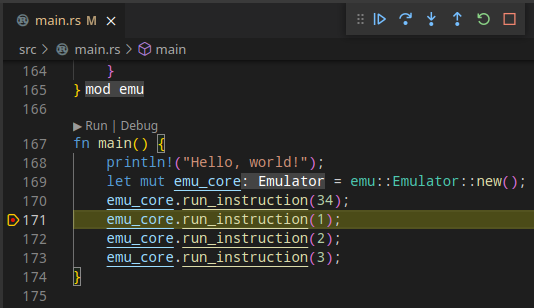
\includegraphics[height=7cm]{step-through-debugging}
              \caption{Step through Debugging with Visual Studio Code.}
          \end{figure}

    \item Register view

          Users should be able to view register values. Visual Studio Code acts as
          a preferred reference of a layout to follow:

          \begin{figure}[H]
              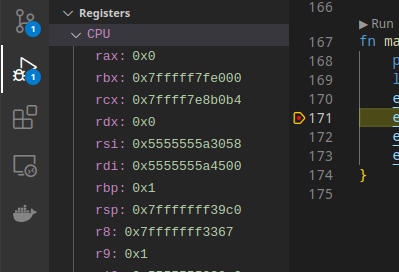
\includegraphics[height=7cm]{vs-code-registers}
              \caption{Visual Studio Code Register View.}
          \end{figure}

    \item Users should be given the option to change the number format for showing
          the contents of the registers between binary, integer, and hexadecimal.
    \item Memory view: Users should be able to view the entire contents of the
          instruction and data memory.
    \item Interactive live view of datapath

          Interactive live view of the emulator datapath with access to inner
          trace contents. A user could hover over various components or traces
          with their mouse to see their current contents. The live view will
          provide the user with how the information is processed and passed
          through each stage. Users should be able to see which stage is active
          with some visual indication.
    \item Mouse hover instruction assistance

          With other IDEs, users can get assistance and documentation by hovering
          their cursor over code they want to understand. For example, if they
          want to know what the C printf() function does, they could hover their
          mouse over the printf() function in their code. In Visual Studio Code,
          and similarly for other IDEs, the functionality may look like Figure
          \ref{fig:vs-code-hover-variable}.

          \begin{figure}[H]
              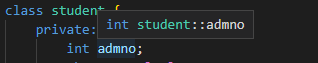
\includegraphics[height=2cm]{vs-code-hover-variable}
              \caption{Mouse hover function and variables assistance.}
              \label{fig:vs-code-hover-variable}
          \end{figure}

    \item The information provided in the hover dialog should include the effect
          of the instruction in pseudocode and any possible limitations to this
          instruction.
\end{itemize}

\subsubsection{Business Requirements}
\begin{itemize}
    \item The interface should be easy to use and familiar for users already
          familiar with Visual Studio Code, Replit, or Godbolt.
    \item The interface should act performant and responsive, where there are no
          frame drops nor stuttering, and selected options give feedback within
          0.1 seconds of interacting.
    \item The interface should act as a logical bridge between the emulation core
          and the parser.
\end{itemize}

\subsection{Parser}
\subsubsection{Requirements}
\begin{itemize}
    \item The parser should be able to properly interpret and tokenize all
          supported instructions, as described in Section
          \ref{subsec:supported-instructions}.
    \item The parser should be able to assemble all supported assembly
          instructions into binary instructions as per the official MIPS64
          instruction set specifications.
    \item Error reporting and detection of invalid assembly code

          The user should be able to see if there are any parts of their assembly
          code that are improperly formatted. This may include using the incorrect
          syntax for a given instruction, using invalid immediate values, or using
          instructions that do not exist in either the project's supported subset
          of instructions or the MIPS64 instruction set as a whole.
    \item Error detection for labels: The parser will return an error if there is
          a J-type instruction that uses a label as an operand that does not match
          any of the labels found throughout the program.
    \item In reporting errors and invalid assembly code to the graphical
          interface, a description of the error and the location in the code
          causing the error should be provided.
    \item When the parser expects an instruction name but receives a string that
          does match any of the instructions that it recognizes, it should be
          considered an error.
    \item If the parser is reading an instruction and expects a label name as one
          of the operands but receives one that has not been defined, it should be
          considered an error.
    \item Suggestions for correct instruction or label when an invalid one is
          recognized

          This falls as an extension to the existing functionality of reporting
          errors. In the event that there are invalid instructions or labels used
          in inputted assembly code, the parser should also be able to give
          suggestions on which instructions or labels to use in replacement. If
          there are instructions or labels with similar names to the invalid ones,
          these will be suggested first before others. The existing error
          recognition for instruction names and label names should still operate
          at a similar level of quality and speed, with or without this feature.
\end{itemize}

\subsubsection{Business Requirements}
\begin{itemize}
    \item Messages and suggestions from the parser should be easy to understand
          for the user by using simple language.
    \item The parser should be able to communicate errors with processing user
          input to the interface for displaying errors at its discretion.
    \item The parser should be able to properly parse and assemble valid input
          code containing less than 50 lines within 4 seconds of being initiated.
    \item The parser should create an API to be used with the graphical interface.
    \item The API used by the parser should be structured in a way that makes
          front-end development as simple as possible.
\end{itemize}

\section{Project Challenges}

One of the challenges that this project faces includes unfamiliarity
with the technology. Each team member has to study Rust and Yew on their
own, not without the additional background knowledge in HTML, CSS, and
JavaScript necessary for front-end development. Furthermore, as SWIM
focuses on the implementation of MIPS64, overall some members will need
to review and understand granular implementation details of the
instruction set architecture. As such, time must be dedicated towards
researching these concepts and finding currently-available options for
MIPS simulators, to understand the scope of functionality and features
that would be added into SWIM. This unfamiliarity with Rust and its
libraries, as well as with the MIPS architecture has initially given the
project a steeper and longer learning curve. There is also an issue with
mobile device support, even though this app is web-based. The formatting
and layout of the page will appear distorted on mobile devices, where
interface items may appear too small to be interactive, or too large to
be functional. In addition, interactivity via touch-based displays can
cause issues with specific Javascript libraries, making this another
potential challenge in project design. This specific instance ultimately
led to the decision of SWIM solely supporting desktop-based browsers and
devices.

Another prominent challenge of this project is less on a technical
level, but it has been found that group members cannot meet consistently
due to their schedules each week during the semester of taking Senior
Design I. The proposed solution was to asynchronously communicate
through Discord, and meeting in any available synchronous times at least
once a week. This has offered increased and consistent communication
between group members outside of weekly meetings. Sharing of materials
and sources between group members becomes easier as a result, but a
problem remains for keeping track of progress. The discord bot DailyBot
assists with this final issue by having members fill out daily standups,
consisting of each members' plan for work of the day, the accomplished
work of the previous day, and any roadblocks that may arise for the day.
From these standups, we have discovered that many members have numerous
personal and educational roadblocks (such as assignments and tests for
other classes, weddings, or extracurricular activities). DailyBot became
unusable after a month of usage due to subscription limitations, however
daily scrums were continued to be tracked manually and has largely no
longer been an issue.

An additional solution to the challenge of meeting time is to create
more meetings within small subgroups of members. In addition to meeting
with the entire group at least once a week, we have found meeting in
smaller groups specific to the area of focus within the program has
allowed for more flexibility and collaboration.

\section{Research - MIPS64 ISA}

With creating SWIM, it is important to have a strong foundational
understanding of the Microprocessor without Interlocked Pipelined Stages
instruction set architecture (MIPS ISA) that this project focuses on.
The following subsections describe various aspects of MIPS64 and some of
the design philosophies built into it.

\subsection{Introduction and Context}

An instruction set architecture (ISA) outlines and specifies the
instructions supported by a given system, as well as the hardware that
those instructions execute on. Informally, an ISA acts as a contractual
communication standard between the hardware and software in a computing
system. The exact instructions and features that are supported vary
between ISAs, but each of them contain core aspects shared by nearly all
architectures. This section aims to outline the instructions, features,
and architecture supported by MIPS, not only for understanding how the
architecture is structured, but for the implementation of SWIM itself.

At its root, SWIM is an application that can simulate a generic MIPS64
processor, complete with compiler, assembler, and live processor
overview. The implementation of such a project directly relies on the
design of MIPS to comply with the standards and approaches established
by it. Without following a documented ISA, this would necessitate
creating a completely new ISA from scratch, which is not only
time-consuming for the scope of this project, but undermines a primary
goal of this project. SWIM is intended to be used as a supplemental
resource in courses whose curricula already focus on MIPS.

\subsection{RISC}

MIPS is considered a ``reduced instruction set computer'' (RISC)
architecture. This is a type of design policy that dictates how
instructions can be structured, which have both merits and drawbacks. A
RISC architecture focuses heavily on using simple processor instructions
that take shorter amounts of time to compute than instructions in
``complex instruction set computer'' (CISC) ISAs. Courses that discuss
introductory computer architecture and design often use RISC
architectures due to this level of simplicity and verbosity. Modern CISC
architectures often reduce their complex instructions into RISC-like
``micro-instructions'' due to their advantages with modern technology
and computation techniques.

For example, to add 1 to the value at memory address 400, a RISC
architecture (such as MIPS) may use the following three instructions to
accomplish this: \texttt{lw t0, 400(0); addi t0, t0, 1; sw t0, 400(0)}.
While this does require multiple instructions (whereas a CISC
architecture would only require one instruction -- \texttt{add [400],
    1}), RISC instructions can generally be processed in a shorter amount of
time, are easier to pipeline, and in the case of multi-cycle datapaths,
have a lower ``cycles per instruction'' (CPI) count.

\subsection{Load-Store ISA}

MIPS is a RISC that is also considered a load-store ISA. A Load-Store
Instruction Set Architecture, as the name suggests, uses load and store
instructions to access the memory. Other instructions use the register
operands (like \texttt{add} for instance) within the ALU, and only those
operations are in the register. This way, not every instruction can
access the memory, only the dedicated loading and storing commands.

\subsection{Addressing Modes}

There are several Addressing Modes in Assembly Language, but the three
main types are: register addressing, immediate addressing, and memory
addressing \cite{tutorialspoint-assembly-addressing-modes}. Immediate
addressing allows for one-to-one address interactions that can happen
immediately like moving data into a register. Register addressing, as
the name implies, addresses the registers' data from the instructions.
Sometimes more than one register addressing is required to access the
data. That is called indirect register addressing. Memory addressing, or
often called direct addressing, has the effective address as part of the
8 bit or 16 bit instruction displacement \cite{gfg-addressing-modes}.

\subsection{Registers}
\label{subsec:mips64-registers}

With the current MIPS64 architecture, there are several registers that
go into the CPU. They include 32 and 64-bit general purpose registers,
the Program Counter, and special registers for multiplication and
division (hi and lo) \cite{mips-specification}. The general purpose
registers are mostly used as source and destination registers for ALU
instructions operations. These registers help the processors output the
results of operations, in either 32 or 64-bits. In this case, since we
are also going to enable MIPS64 support for the emulator, the MIPS64
processor will, naturally produce 64-bit results, even if the
instructions' format are fixed within 32-bit.

\begin{figure}[H]
    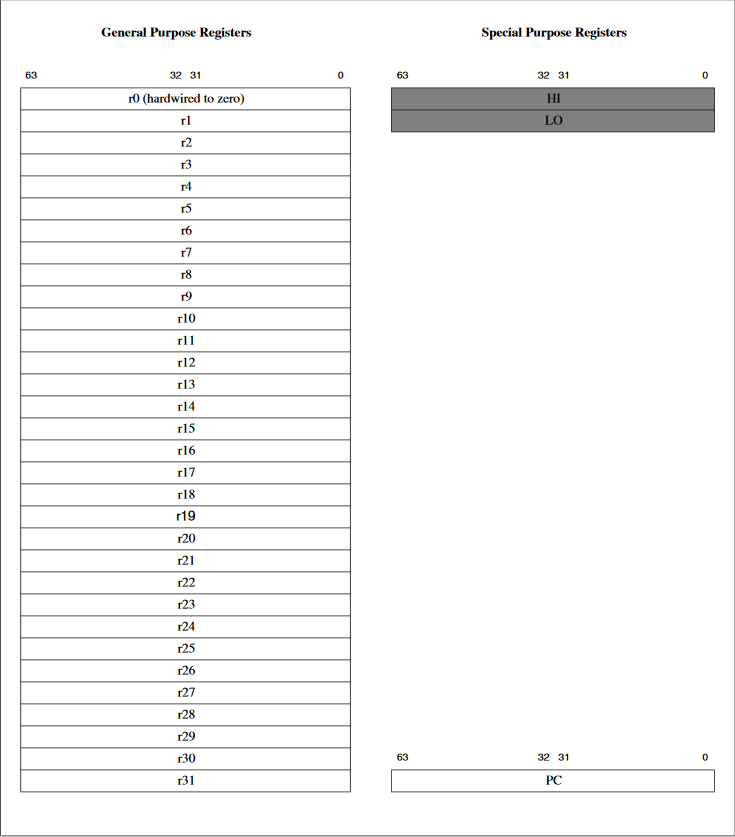
\includegraphics[height=16cm]{mips64-register-layout}
    \caption{Layout of registers for MIPS64, according to \protect\cite{mips-specification}.}
\end{figure}

\begin{figure}[H]
    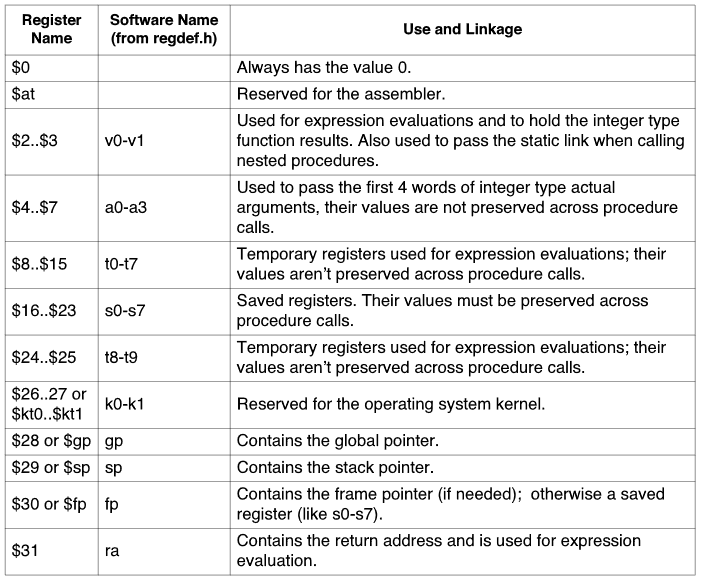
\includegraphics[height=11cm]{gpr-names}
    \caption{Use and linkage of each of the 32 64-bit general-purpose registers, as according to \protect\cite[Table~1-1]{mips-programmers-guide}.}
\end{figure}

\begin{figure}[H]
    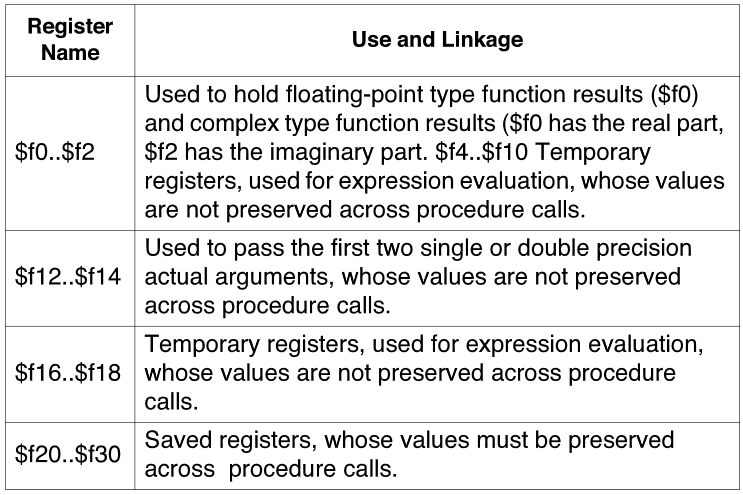
\includegraphics[height=8cm]{fpr-names}
    \caption{Use and linkage of each of the 32 64-bit floating-point
        registers, as according to \protect\cite[Table~1-3]{mips-programmers-guide}.}
\end{figure}

\subsection{Assembly Format}

All of MIPS' format is encoded in binary, as computations and operations
deal with binary arithmetic and logical shifts with or without
conditions. All of MIPS instructions are 32-bit long, and subsequently,
there are 32 registers used in MIPS. The first 6 bits of the instruction
is called the opcode, which identifies what type and what operation the
instruction is carrying out. There are 3 instruction formats that will
be discussed in the next section: R-Type, I-Type and J-Type.

\subsection{Instruction Format}

General format (fixed 32-bit):

\emph{R-type:}

\begin{tabularx}{\textwidth}{|C|C|C|C|C|C|}
    \hline
    Opcode: 6 bits & rs (source register): 5 bits & rt (source register): 5 bits & rd (destination register): 5 bits & shamt (shift amount): 5 bits & funct: 6 bits \\
    \hline
\end{tabularx}

All R-Type instructions have an opcode of 0, which is 000000 in 6 bits.
The shift amount is only used in shift operations. The \texttt{funct}
field specifies which R-type function is being used, although the slot
itself is not used much. This format has exceptions that lie within
multiplying and division including modulus.

R-Type Operations: (\$s0 is rd, \$s1 is rs, \$s2 is rt)

\begin{itemize}
    \tightlist
    \item add \$s0, \$s1, \$s2 =\textgreater{} \$s0 = \$s1 + \$s2
    \item sub \$s0, \$s1, \$s2 =\textgreater{} \$s0 = \$s1 - \$s2
    \item and \$s0, \$s1, \$s2 =\textgreater{} \$s0 = \$s1 \& \$s2
    \item or \$s0, \$s1, \$s2 =\textgreater{} \$s0 = \$s1 \textbar{} \$s2
    \item xor \$s0, \$s1, \$s2 =\textgreater{} \$s0 = \$s1 \^{} \$s2
    \item nor \$s0, \$s1, \$s2 =\textgreater{} \$s0 = \textasciitilde(\$s1
          \textbar{} \$s2)
    \item slt \$s0, \$s1, \$s2 =\textgreater{} \$s0 = 1 if \$s1 \textless{} \$s2,
          \$s0 = 0 otherwise
    \item sll \$s0, \$t0, 1 =\textgreater{} \$s0 = \$t0 * 2\^{}1 \item srl \$s0, \$t0, 2 =\textgreater{} \$s0 = \$t0 / 2\^{}2
\end{itemize}

Special R-Type instructions:

\begin{itemize}
    \tightlist
    \item mult \$t0, \$t1 =\textgreater{} ``product register'' (hi or lo) = t0 *
          t1
    \item div \$t0, \$t1 =\textgreater{} hi = t0 \% t1, lo = t0 / t1
\end{itemize}

\emph{I-type:}

\begin{tabularx}{\textwidth}{|c|c|c|C|}
    \hline
    Opcode: 6 bits & rs: 5 bits & rt: 5 bits & const or address: 16 bits \\
    \hline
\end{tabularx}

Each I-Type instruction has a unique opcode. Register rt may be a source
or a destination. The constant or address in 16 bits is called an
``immediate'' source, hence the I in I-Type.

I-type Operations:

\begin{itemize}
    \tightlist
    \item addi \$s0, \$s1, 10 =\textgreater{} \$s0 = \$s1 + 10
    \item andi \$s0, \$s1, 11 =\textgreater{} \$s0 = \$s1 \& 11
    \item ori \$s0, \$s1, 12 =\textgreater{} \$s0 = \$s1 \textbar{} 12
    \item slti \$s0, \$s1, 13 =\textgreater{} \$s0 = 1 if \$s1 \textless{} 13,
          \$s0 = 0 otherwise
    \item lw \$t0, 16(\$s1) =\textgreater{} \$t0 = Mem{[}\$s1 + 16{]}
    \item sw \$t7, 48(\$s5) =\textgreater{} Mem{[}\$s5 + 48{]} = \$t7
    \item beq \$t0, \$t4, Label =\textgreater{} if \$t0 == \$t4, goto Label
    \item bne \$t0, \$t4, Label =\textgreater{} if \$t0 != \$t4, goto Label
\end{itemize}

\emph{J-type:}

\begin{tabularx}{\textwidth}{|c|C|}
    \hline
    Opcode: 6 bits & Target address: 26 bits \\
    \hline
\end{tabularx}

J-type instructions are basically jump commands. J-type instructions
have opcode of 2 (000010) and 3 (000011):

\texttt{j} is an unconditional jump that does not need registers and
modifies the Program Counter as it executes. For example \texttt{j
    Label} means go to Label. Another J-Type instruction is \texttt{jal},
which means Jump And Link.

\subsection{MIPS64}
\label{sec:mips64}

MIPS64 is an extension to the MIPS ISA that allows for computation and
the use of 64-bit memory addresses, general purpose values, and
floating-point values.

\subsubsection{Co-processor}

MIPS' coprocessors are all grouped into a MIPS processor, and as of
MIPS64, the coprocessors handle different things within the system, and
without them, MIPS would cease to operate. There are a total of 4
coprocessors provided by the architecture, numbering from 0 to 3.

Coprocessor 0, or CP0, is the foundation of the processor. CP0's job is
to control the system, which includes memory management, exception
handling, keeping cache addresses and manipulating them, as well as
being responsible for some of the CPU's setup just to name a few.

The remaining three coprocessors are used as floating point units, with
CP2 being ``implementation-specific,'' which means CP2 is only available
as a floating point for certain implementations of the MIPS architecture
\cite[p.~74]{mips-specification}. The floating point units are used to
move instructions to and from the coprocessor, and there are specialized
instructions for these coprocessors to use the opcode space for those
tasks. However, for the floating point units to work, CP1 needs to be
activated by CP0, or else it will return an exception.

\subsubsection{Registers and Additional Instructions}

Compared to the standard 32-bit MIPS architecture, MIPS64 specifies all
general-purpose registers to use 64-bit registers, and adds 32, 64-bit
floating-point registers.

Additional instructions are available to the processor, including
\texttt{add.s} (add single-precision floating-point), \texttt{mtc1}
(``move to coprocessor 1''), and \texttt{c.eq.d} (``compare if equal,
double-precision floating-point''). These instructions intended for the
coprocessor use an alternative instruction format to those formats
previously listed.

\begin{figure}[H]
    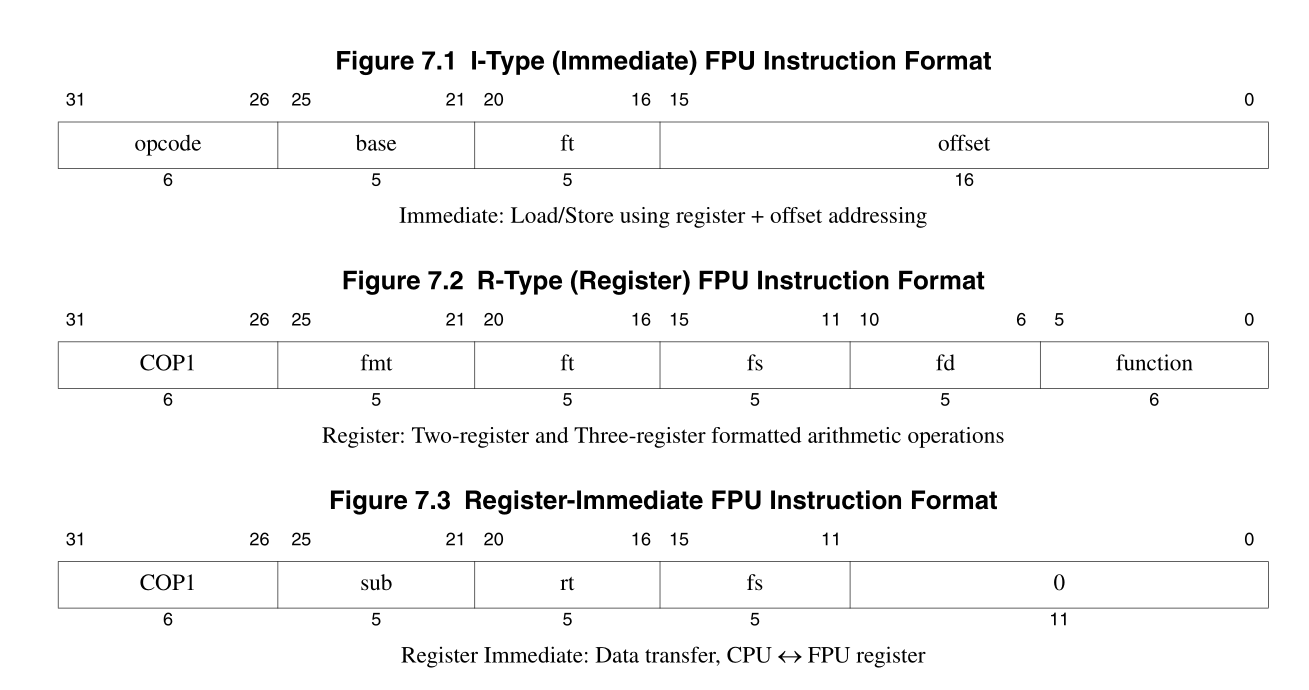
\includegraphics[height=8cm]{fpu-instruction-formats}
    \caption{Floating-Point Unit Instruction Format, from \protect\cite{mips-specification}.}
\end{figure}

Of note is that for instructions indicating ``COP1'' in the traditional
``opcode'' field, this is equivalent to 010001\textsubscript{2}
(17\textsubscript{10}).

For floating-point instructions that utilize the \emph{fmt} field, this
represents the format of the data being handled. For example, the
difference between \texttt{add.s}, \texttt{add.d}, \texttt{add.ps}.

\begin{figure}[H]
    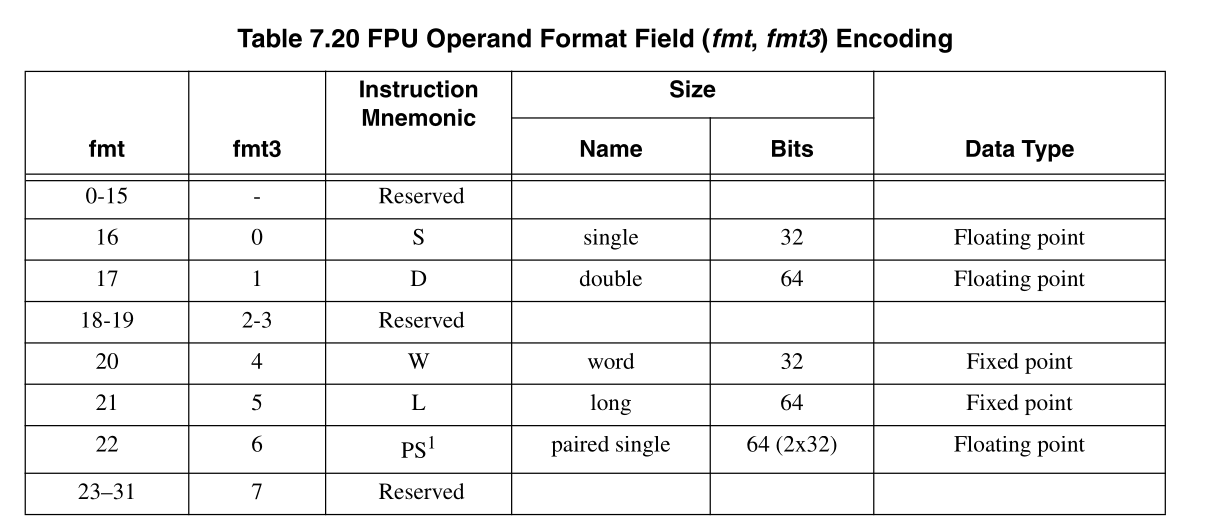
\includegraphics[width=\textwidth]{fpu-fmt-encoding}
    \caption{Floating-point unit fmt field encoding, from \protect\cite[Table~7.20]{mips-specification}.}
\end{figure}

Notice that all applicable formats have the uppermost bit of the
\emph{fmt} set as 1 in this case. Cases where this bit is 0 should be
considered for a different instruction.

For floating-point instructions that utilize the \emph{cond} field, this
represents the type of comparison being made by a floating-point unit.
For example, the difference between \texttt{c.eq.s}, \texttt{c.ne.s},
and \texttt{c.gt.s}. See Figure \ref{fig:fpu-cond-encoding} for the
possible values for this field.

\begin{figure}[H]
    \begin{minipage}{\textwidth}
        \begin{center}
            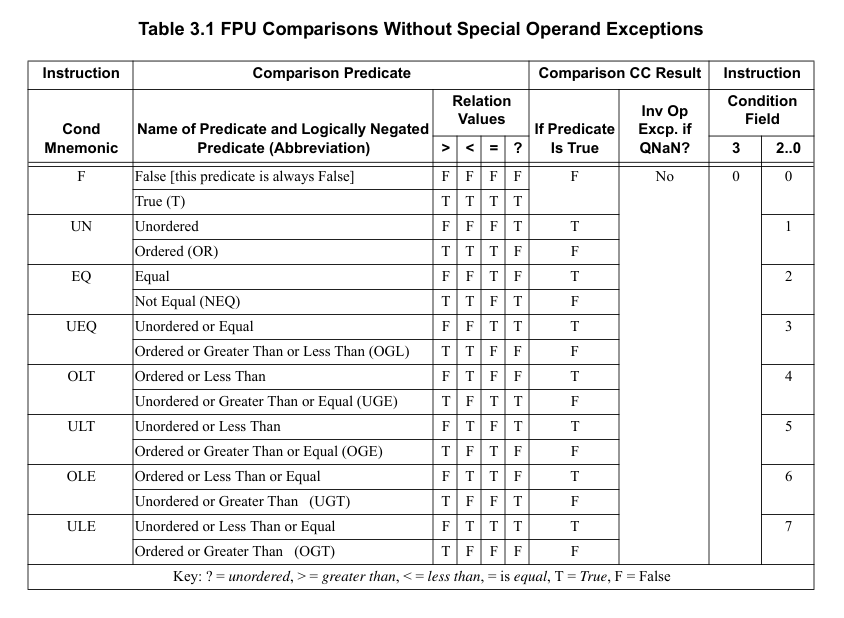
\includegraphics[width=0.85\textwidth]{fpu-cond-encoding-1}
            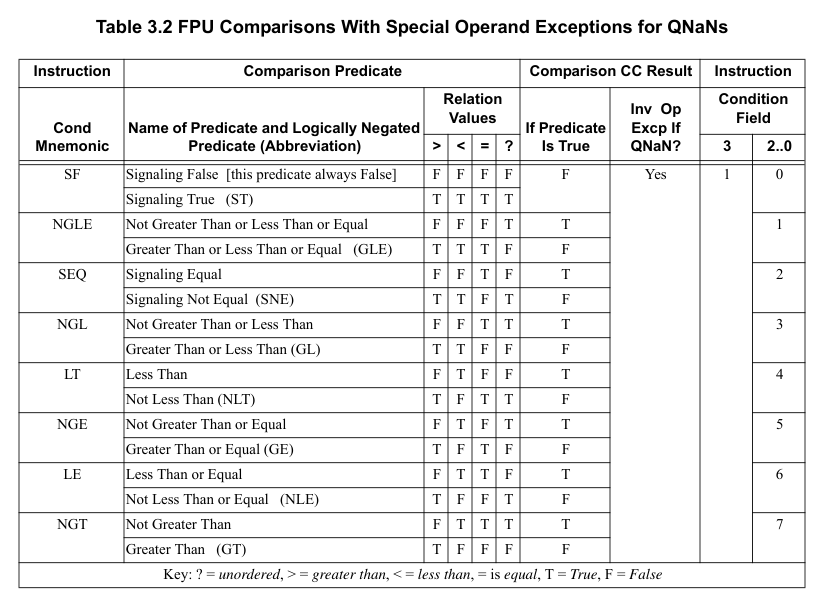
\includegraphics[width=0.85\textwidth]{fpu-cond-encoding-2}
        \end{center}
    \end{minipage}
    \caption{Floating-point unit comparison field encoding, from \protect\cite{mips-specification}.}
    \label{fig:fpu-cond-encoding}
\end{figure}

Notice that conditions are paired. To find if the first item in the pair
is true, use the \texttt{bc1t} (branch on coprocessor 1 true)
instruction. To find if the second item in the pair is true, use the
\texttt{bc1f} (branch on coprocessor 1 false) instruction.

The following describes the instruction format used in the ``Floating
Point Compare'' instruction.

\begin{itemize}
    \tightlist
    \item fmt - The format of the registers being compared.
    \item ft and fs - The floating-point registers being compared.
    \item cc (``condition code'') - Selects which condition code will be written
          to. (It will be set to 0 in all cases for this implementation.)
    \item cond - Specifies the type of comparison being made.
          \begin{itemize}
              \tightlist
              \item Bit 3 - Indicates whether the instruction should signal an exception on
                    QNaN inputs. (Exceptions are ignored for this implementation.)
              \item Bits 2-1 - The nature of the comparison (e.g. greater than, equal to).
              \item Bit 0 - Specifies whether the comparison is ordered or unordered, that
                    is, false or true if any operand is a NaN.
          \end{itemize}
    \item FC = 11 (``function code'') - Indicates that this is the comparison
          function.
\end{itemize}

The following are the \emph{cond} codes applicable for this
implementation. Keywords to the right do not exist as real instructions,
but instead are mnemonics. To use those, the \texttt{bc1f} instruction
should be used with the corresponding real instruction.

\begin{itemize}
    \tightlist
    \item 0010 - \textbf{eq (equal)} // use bc1f for \textbf{neq (not equal)}
    \item 1100 - \textbf{lt (less than)} // [nlt - not less than]
    \item 1101 - [nge - not greater than or equal] // use bc1f for \textbf{ge (greater than or equal)}
    \item 1110 - \textbf{le (less than or equal)} // [nle - not less than or equal]
    \item 1111 - [ngt - not greater than] // use bc1f for \textbf{gt (greater than)}
\end{itemize}

\section{Research - Web Development in Rust}

Rust, in general, is a relatively recent programming language, being
originally released in 2010 \cite{asay2021}. As such, it has modern
features such as its borrow checker that makes development more secure.
The Rust borrow checker, essentially replacing the garbage collection
used in other languages, manages ownership by assigning an owner to each
variable, where that variable may only have one owner at a time
\cite{rust-book-ownership}. This implies that the owner can be changed,
as long as the variable is still available within some scope. Should a
variable reach the end of its scope, the borrow checker will drop the
value from used memory (akin to garbage collection). One advantage of
the borrow checker is that there become defined points in code where it
is safely determined a piece of data is no longer being used. Functions
may use references to variables made by ``borrowing'' a variable,
meaning in this case going out of scope does not correlate to lost
ownership \cite{rust-book-borrowing}. The borrowed reference instead is
returned to its original owner when the scope of the borrow finishes.
This system of borrow checking allows Rust to pitch itself as a
programming language perfect for low-level and embedded systems. As SWIM
is primarily intended to emulate a MIPS processor, this was a deciding
factor to using Rust.

Despite Rust having high praise for its static borrow checking, some of
Rust's functionalities make development difficult based on these same
concepts. Data types are more rigid and access to data is more
restrictive than in other languages.

To understand how to develop a web application with Rust, a number of
components are involved to make this process approachable for
development. The following subsections outline the research completed to
use Rust for SWIM's planned feature set.

\subsection{Using WebAssembly}

This project is unique in that rather than using the standard JavaScript
framework like React, Angular, and Vue to build the front end, it is
utilizing a new type of code to build web applications, WebAssembly. As
the development team explains,

\begin{quote}
    ``WebAssembly (abbreviated Wasm) is a \emph{safe, portable, low-level
        code format} designed for efficient execution and compact
    representation. Its main goal is to enable high performance applications
    on the Web, but it does not make any Web-specific assumptions or provide
    Web-specific features, so it can be employed in other environments as
    well.'' \cite{webassembly-introduction}
\end{quote}

Historically, HTML, CSS, and JavaScript were the only means to run
applications on web browsers and it has been the standard for almost 20
years. WebAssembly aims to allow programmers to write in other
languages, like Rust, and compile to a binary file that could run on the
web. This is still in its infancy, so one of the biggest challenges is
how our project may change as WebAssembly matures.

WebAssembly code is packaged in an Assembly-like language, represented
in either binary data corresponding to instructions, types, etc. as a
.wasm file or human-readable text (.wat). The language is designed to be
independent of programming languages, computer hardware, and the browser
it runs on. Currently, WebAssembly is supported on Google Chrome,
Microsoft Edge, Mozilla Firefox, and Apple Safari, limiting legacy
browser users from using SWIM. It is important to note that Chrome and
Firefox have FOSS forks that could run WebAssembly, but support for
these forks varies, since WebAssembly is only supported by the more
recent versions of the four aforementioned browsers
\cite{mdn-webassembly}. Additionally, WebAssembly was never meant to
replace JavaScript, as it is synonymous with web development, but they
can be used together to improve the user's experience on the web with
WebAssembly's speed and JavaScript's libraries and tools. As an example,
Figma, the tool we used to design our UI, was developed using C++ and
Enscripten to export to asm.js, and later switched to WebAssembly to
take advantage of its speed for loading in documents
\cite{figma-webassembly, madewithwebassembly-figma}. However, the
implementation resulted in the app being unusable exclusively for Google
Chrome users. The two bugs were failing to cache the translated
WebAssembly code, also it would crash due to the app accessing
WebAssembly's memory limit. The first would force Chrome to reload the
translated code resulting in slower performance and the second made the
app unusable in inconsistent intervals \cite{chromium-webassembly-bug1,
    chromium-webassembly-bug2}. Fortunately, both of those bugs are fixed
within months.

In order for Rust and WebAssembly to work
\cite{wasm-game-of-life-introduction}, the project requires us to have
the most recent version of Rust's toolchain (rustup, rustc, and cargo),
wasm-pack, cargo-generate, and npm. wasm-bindgen is required as a
dependency in the project's .toml file, then you can use wasm-pack to
build your project. By typing in \texttt{wasm-pack build} in the main
directory of your project via terminal/cmd, WebAssembly will generate a
.wasm, .js, .json, and .ts file in the package directory. Within the
package directory, you run the following npm commands:

\begin{enumerate}
    \tightlist
    \item \texttt{init wasm-app} \textless new subdirectory\textgreater, to produce the
          appropriate .json, .config.js, .html, and .js in the new subdirectory.
    \item \texttt{install}, to ensure the local development server and its dependencies are
          installed.
    \item \texttt{run start}, to run the web application locally. If you want to see any
          changes made through the web application, run \texttt{wasm-pack build} in the
          main directory then refresh the page.
\end{enumerate}

\subsubsection{Using \texttt{wasm-pack} \& \texttt{wasm-bindgen}}
\label{subsec:pack-bindgen}

With \texttt{wasm-pack} \cite{wasm-pack} being used for building, Rust
WebAssembly packages could be published to the npm registry or allow it
to be used alongside any JavaScript packages already well-established.
This interoperability is integral to incorporating a new framework such
as Rust with existing JavaScript projects. \texttt{wasm-bindgen}
\cite{wasm-bindgen} is a Rust library and CLI tool that facilitates
high-level interactions between wasm modules and JavaScript. However,
there are some limitations on which JavaScript libraries you can bind
with it. You cannot use JavaScript libraries that are post-processed,
like ones that are processed through Babel(i.e. FileSaver.js), rather
they have to be handwritten. There are two additional crates that helps
with WebAssembly binding JS's API libraries, and they are packaged with
wasm-bindgen:

\begin{enumerate}
    \tightlist
    \item \texttt{js-sys} \cite{js-sys} provides raw bindings to all the global APIs guaranteed to
          exist in every JavaScript environment by the ECMAScript standard. With
          it, we can work with JS types without writing the imports by hand. This is key to pass in objects,
          arrays, and values to JavaScript libraries in Rust since both do not share types.
    \item \texttt{web-sys} \cite{web-sys} provides raw wasm-bindgen imports for all of the Web's
          APIs, so the required APIs for our project like DOM, Console, and UI
          Events are supported here.
\end{enumerate}

\subsubsection{Thoughts on WebAssembly}

While WebAssembly is a great innovation for web development, its
learning curve is steep given the time available to study and use it
effectively. While working on a miniature project with WebAssembly, a
huge issue was encountered with code organization and understanding of
the available tools. The documentation is expansive since the
aforementioned crates have to support all JavaScript API calls, and some
of them are not necessary to our current goals. While this is not
without its merits, it will take additional time through the development
of the project to learn about WebAssembly's full capability.

Since WebAssembly is still new in the web development ecosystem, there
are a few methods to incorporate it on the Web. According to the MDN web
docs for WebAssembly, ``porting a C/C++ application with Emscripten,
writing or generating WebAssembly directly at the assembly level,
writing a Rust application and targeting WebAssembly as its output, and
using AssemblyScript which looks similar to TypeScript and compiles to
WebAssembly binary'' \cite{mozilla-webassembly-concepts} are the main
entry points to incorporate it into web applications.

Despite the challenges that come with WebAssembly, it has the advantage
of any assembly language, where binary data can be disassembled into
text, and this can be further converted with a decompiler to readable
code. This allows developers to debug and understand web applications
that utilize WebAssembly. However, this is only useful if the developer
understands WebAssembly's instruction set, and if a decompiler can
provide a 1:1 translation of code and text, the latter being especially
difficult given the loss of information associated with compiling.

\subsection{Using Yew}

While WebAssembly provides an environment for programming languages to
be used in web development, there are more steps involved to get a web
application developed, so we selected Yew as our framework. Yew is
comparable to React, as it is component-based, which aids in building
interactive UIs for web applications. Yew has excellent performance
compared to other web frameworks since it minimizes DOM API calls and
offloads processing to background threads using web workers. It also has
JavaScript interoperability which allows users to leverage Node.js
packages and to integrate with existing JavaScript applications
\cite{malomo2022}.

Having a framework like Yew to use on top of WebAssembly is beneficial
for development, since WebAssembly's learning curve is comparatively
steep. Developing in WebAssembly and JavaScript to incorporate features
directly can make the project's code cumbersome and ineffective.
Instead, Yew aims for developers to use a programming language like Rust
to build the web application, while the translation to WebAssembly and
JavaScript are abstracted to libraries.

\subsubsection{Yew's Components Model}

One of Yew's defining features is how it streamlines web application
development; it uses a lifecycle model for struct components. Struct
components manage their state and render themselves to the DOM, which is
where the user will interact with SWIM's HTML. The lifecycle, taken from
Yew's Documentation \cite{yew-lifecycle}, is as follows:

\begin{enumerate}
    \tightlist
    \item Create -- The component receives properties from its parent component
          and stores them within itself. This initializes its state and creates a
          link that can be used for callbacks or sending messages.
    \item View -- This describes how the component should be rendered to the DOM.
          Yew has an \texttt{html!} macro for declaring HTML and SVG nodes, and
          attributes and event listeners can be attached to them. The macro is
          similar in function to React's JSX, but allows shorthand syntax for
          readability.
    \item Rendered -- Once the \texttt{view} method is called, this method will
          render the results from the component's view method to the DOM, but
          before the browser refreshes the page. This is useful when you want to
          perform actions that can only be completed after the component has
          rendered elements. A few situations where this is applied to SWIM are
          getting the values from the core and displaying them in their respective
          areas and displaying error messages from the parser.
    \item Update -- This is where the communication between components occurs and
          a component may update and re-render itself based on received messages.
          These messages can be sent by event listeners, child components, Agents,
          Services, or Futures. Agents are used to offload tasks to web workers.
          Services for interacting with external resources like mouse/keyboard
          events, geolocation changes, output from an external JavaScript library,
          and WebSocket messages. Futures are Rust's representation of an
          asynchronous operation's success (or failure) and its value; this is a
          concept borrowed from JavaScript's \texttt{Promise} objects.
    \item Changed -- This eases the parent-to-child node communication by only
          changing the values of a property.
    \item Destroy -- This is for general clean-up of the component's prior
          actions, and it automatically does this once the component is unmounted
          from the DOM.
\end{enumerate}

It is possible to implement infinite loops by updating the struct
component after every render when the update also requests the struct
component to be rendered. This is done by setting the \texttt{update}
method to {\em true} to always request to re-render on any message from
the \texttt{rendered} method. This lifecycle could make the
implementation process easier for the back end of this project. A good
example is implementing a live debugger in SWIM, and this can easily be
done by running the parser in an infinite loop so it can catch whenever
the user mistyped an instruction or try to access memory that would
cause the virtual machine to crash upon execution.

An alternative to struct components are function
components\cite{yew-function-components}. These are more abstract than
struct components in that all the code is going into the equivalent of a
struct component's \texttt{view} method, but the code is more concise.
Then, Yew builds a virtual tree of these components to compute the
virtual DOM. When an update is necessary, Yew will call the view
function with the new virtual DOM and only propagate the
new/changed/necessary parts to the actual DOM.

The components only have two associated types: Message and Properties.
The Message type is used for a component to send messages after an event
has taken place, like a button being clicked. A Message, in
implementation, is an enum where each variant is an event to be handled
by that component, making handling multiple types of events in a
component easier to develop and implement. The Properties type
represents the information passed to a component from its parent.
Properties is a trait that must be implemented, and specifies whether
properties are required or optional. This type is used when a component
is being created or updated, as new values of component properties can
be provided during these instances. With both Message and Properties, it
is wise to keep them in the corresponding component's module and stay
encapsulated there.

Callbacks are the primary method of communication, and they are usually
located in the \texttt{view} function within a component with the
actions to initiate the communication stored inside the \texttt{html!}
macro. The handler function passed to \texttt{callback} must always take
a parameter, which is usually a type of a UI Event. An example of this
is shown in Yew's sample code with the \texttt{onclick} handler, being
rendered as a button, requires a \texttt{callback} to the
\texttt{AddOne} message to tell the component to add one to
\texttt{value} upon the button being clicked on. With that in mind, the
handler can determine what kind of message to be sent to the component
then the message is scheduled for the next update loop regardless. In
order for the callback to not cause any updates,
\texttt{batch\_callback} can be used to create conditionals for which
message to send.

\begin{figure}[H]
    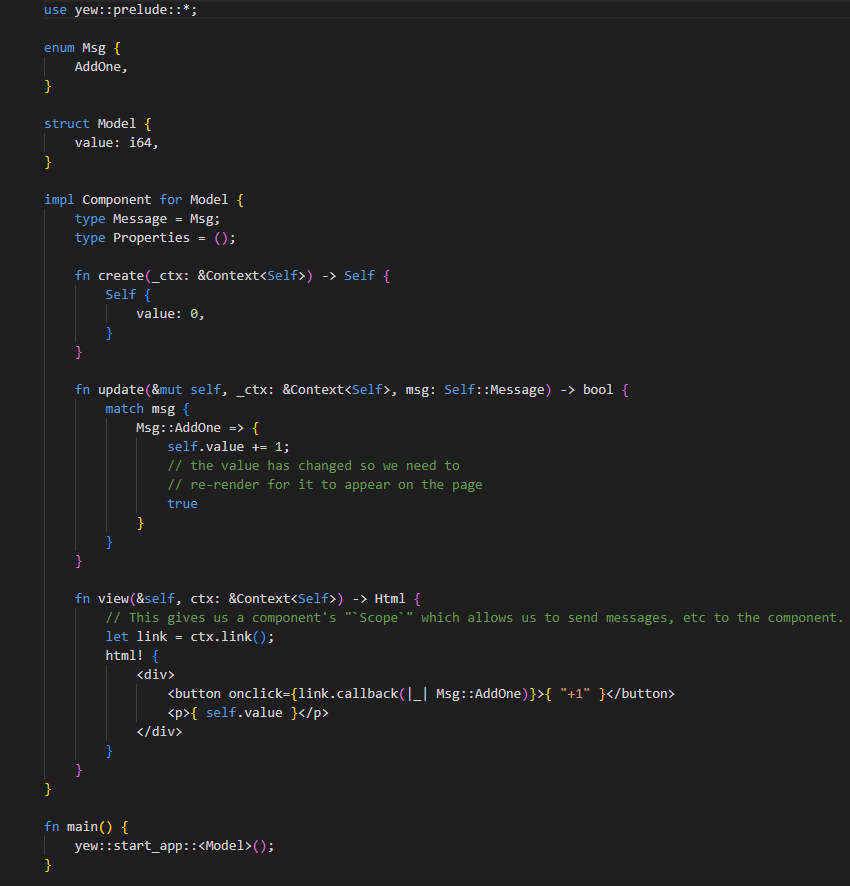
\includegraphics[height=14cm]{yew-sample-code}
    \caption{Yew's sample app code to show how the lifecycle model improves readability and how certain components behave through callbacks.}
\end{figure}

\subsubsection{The \texttt{html!} Macro} \label{subsec:html-macro}

Yew's \texttt{html!} macro, as stated before, allows writing HTML and
SVG code directly into Rust, and the rules for using valid HTML tags
still apply here. The macro helps explicitly specify what will be
rendered on the webpage through the DOM API.

There are a few caveats with \texttt{html!} compared to normal HTML. For
example, consider an html button\texttt{ \textless button onclick =
    \{onclick\_list\}\textgreater Show\textless/button\textgreater}. This
syntax is valid in html, but it will throw an error in \texttt{html!}.
The correct \texttt{html!} format is \texttt{\textless button onclick =
    \{onclick\_list\}\textgreater\{"Show"\}\textless/button\textgreater}. As
seen in this example, the syntax between HTML and \texttt{html!} can be
different. While the compiler will show how HTML can be changed to
\texttt{html!} for specific syntax errors, the macro can be a little
jarring to use for novice HTML developers.

\subsubsection{Thoughts on Yew}

What was discussed in this subsection are only the significant topics
that pertain to the general understanding of Yew's code and feature
structure. Yew assists with the translation process to WebAssembly by
having little-to-no developer interaction with JavaScript, as this
interaction is generated from the Rust code. At this point, Yew is close
to being in release state, so it is safe to assume that our project will
not be heavily affected by updates. At worst, we will refactor the code
to be in-line with the most recent release of Yew. We relied on web-sys
for the API calls, however the documentation is vast to account for all
the APIs supported by JavaScript and using it is diffucult to read and
understand due to its verbose nature. There are crates that will remedy
this issue, but utilizing web-sys is inevitable to interact more
intimately with the APIs. The documentation for Yew is hard to follow,
but there are examples that show the concepts in action, video tutorials
on the framework, and a discord server emcompassing everything about Yew
\& Rust web development. Yew has a lot of support compared to its
contemporaries, there are plenty of real-world examples that used Yew as
a framework to develop their apps. One example is qubit \cite{qubit},
which is a calculator that could do algebra, conversions, and functions.
It would update the output based on the user's input automatically. The
parser used in this project was pest \cite{pest}, which is a parsing
library that allows developers to easily create a parser and define a
grammar. While pest may be appealing in other applications, it will not
be used with SWIM since a custom parser was deemed to be more capable of
understanding MIPS syntax and pseudo-instructions, as well as
interacting with the emulation core and front end.

\subsubsection{Using Trunk}

Yew uses Trunk \cite{trunk}, a WebAssembly web application bundler for
Rust, which streamlines the development process, as Trunk can be used to
detect changes on the filesystem and automatically trigger new builds by
enabling the \texttt{watch} parameter. It runs \texttt{cargo build} on
the project targeting the wasm32 instruction set, runs
\texttt{wasm-bindgen} on the assembled .wasm, and spawns asset build
pipelines for any assets defined in the target \texttt{index.html}.
Trunk's specialty is using a source HTML to drive all asset building and
bundling, which makes the project look cleaner at the top-most level.
With Trunk, SWIM's source code, and a compatible web browser, you will
be able to run SWIM on your computer locally.

\subsubsection{Using Gloo}

Gloo \cite{gloo} is a toolkit to abstract JavaScript API calls to simple
functions. It works by providing a collection of crates that can be
added based on the specific API calls needed. While the calls are
``simplistic,'' they are wrappers to \texttt{web-sys} calls. This
implies that during development, one may need to read both the
documentation for the specific Gloo crate and the JavaScript API
documentation to gather a complete understanding of its implementation.
It may come into question at this point the number of layers of
abstraction needed for SWIM's development, especially since the majority
of the calls are housed in the \texttt{gloo-utils} crate which would be
used for calls to the DOM API. However, the advantage of more readable
code from an outsider's perspective is preferred since the function
calls are labeled idiomatically.

The following describe the crates we have used while working on SWIM,
provided by Gloo:

\begin{itemize}
    \tightlist
    \item Console -- This crate gives us access to the browser's console for
          logging information onto it, clearing it, and more. It was used as a
          means to debug communications between the front end, parser \&
          assembler, and emulation core.
    \item Dialogs -- This crate allows the user to interact with the program by
          asking for input, alerting them of a certain event, or confirming a
          selection. This appears to be useful for creating a small help section
          with a browser's `alert` feature, but this should not be abused, as
          users should not click through many windows to do a simple task.
    \item Events -- This crate is for implementing event listeners to user actions
          like mouseover, keyup, etc. This was used primarily in the
          implementation of the visual datapth.
    \item File -- This crate is for supporting file read and write, which could be
          useful for loading code stored locally on one's computer.
    \item Utils -- This crate houses convenience functions to access web\_sys
          bindings. This means we use web\_sys idiomatically to access APIs that
          are not supported by gloo, then we can use this to improve readability.
          Due to that previous fact, the documentation fallbacks on web\_sys which
          is huge given its nature. As mentioned before, it is recommended that we
          compare the documentation to the one provided by Mozilla.
\end{itemize}

\subsection{Monaco}
\label{subsec:monaco}

The open-source library Monaco, developed by Microsoft \cite{monaco}, is
the key to making the editing experience of users similar to software
they have already used. In practice, Monaco is used as the editor in the
popular editor Visual Studio Code. The library comes included with all
the major features a developer might expect when using a modern code
editor, such as syntax highlighing, IntelliSense, and inline error
messaging. With its popularity, many users of Monaco apps feel
comfortable and familiar, which is ideal for use with SWIM.

The feature set of Monaco fits well with SWIM, as there should be ample
user assistance such as error highlighting, tab completion, and
suggestions. Monaco comes with a usable API for providing these
features, which in one example, is particularly important for supporting
step-through execution with line highlighting. Monaco also has a
built-in auto-commenting feature, where a single button combination can
be pressed when selecting text to comment said text {[}Ctrl/Cmd + K +
C{]}.

By default, code syntax highlighting works in Monaco without
modification. If this were not the case, it is even possible to markup
and support syntax highlighting for custom programming languages
\cite{monaco-custom-languages}. Monaco performs syntax highlighting with
the help of the Monarch library \cite{monarch}. This custom syntax
highlighting can come into importance, should support for different MIPS
dialects be desired in future iterations of the project.

\begin{figure}[H]
    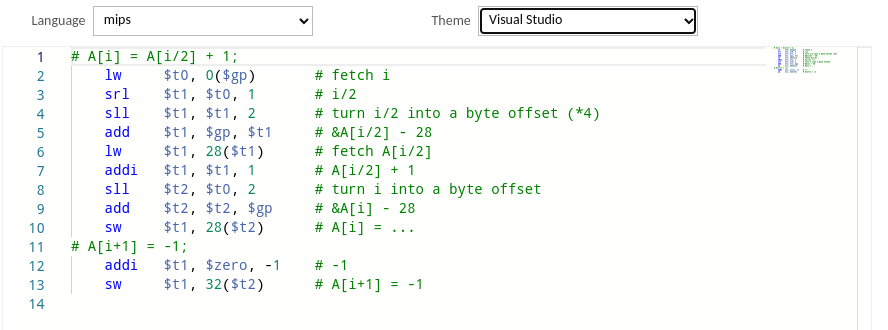
\includegraphics[width=\textwidth]{monaco-mips-syntax-highlighting}
    \caption{MIPS syntax Highlighting Inside Monaco}
\end{figure}

An additional feature of Monaco is tab completion, which is crucial for
many developers, often present in popular editors such as Visual Studio
Code, Vim, or Atom. Those new to a language or framework often use tab
completion and other assistance tools to help in writing code, and even
more experienced developers may choose to use tab completion to increase
their code output speed. At a minimum, Monaco will recognize patterns in
code, it will then use these patterns to provide suggestions. With some
configuring, it would be possible to give code suggestions in SWIM based
on a particular MIPS instruction. For example, after writing an
instruction, a register usually will come next, so a pop-up box could
suggest registers to type. For jump and branch instructions, the editor
may suggest labels to use. This suggestion feature is a stretch goal of
SWIM.

\begin{figure}[H]
    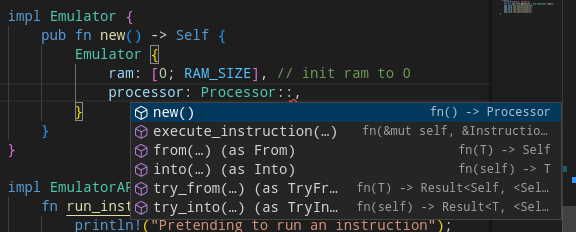
\includegraphics[height=5cm]{monaco-suggestions}
    \caption{A code suggestion in Visual Studio Code, an IDE that uses the Monaco library.}
\end{figure}

The API for Monaco, while extensive, can be difficult to read or parse
through. Due to the common naming conventions used by Microsoft, unlike
in other languages, names can be overly-descriptive and complex, as
documented on the Microsoft website \cite{monaco-api}. The library is
feature-rich, which requires coordination to use them to their fullest.
Despite this, Monaco has become a popular library, and with this
popularity comes more experience and help from other developers via
online forums. There are different tutorials on using Monaco from
developers as well \cite{mishka-monaco, sahoo2018}.

The Monaco editor is written in TypeScript and its API is written in
JavaScript. While Rust will be the primary language used in SWIM, the
following section describes how Monaco can be interfaced with.

\subsubsection{rust-monaco}

\texttt{rust-monaco} \cite{rust-monaco} is a crate that provides
bindings between Monaco Editor and Rust via \texttt{wasm-bindgen}. In
order to fully understand its API calls for development, Monaco's
documentation must be referred to in addition to the documentation for
the Rust bindings \cite{rust-monaco-docs}, as documentation is currently
only 78 percent complete at the time of writing. rust-monaco does allow
developers to implement new options and features that may not yet be
explicitly bound with this crate.

The following outline the currently available modules for the
rust-monaco crate:

\begin{itemize}
    \tightlist
    \item api -- This is where all the wrappers for the JavaScript code for
          Monaco's settings are in. The main struct to create the window is called
          \texttt{CodeEditorOptions} and the translation between Rust and
          JavaScript is quite simple with the comparison shown in Figure
          \ref{fig:monaco-initialize}.

          \begin{figure}[H]
              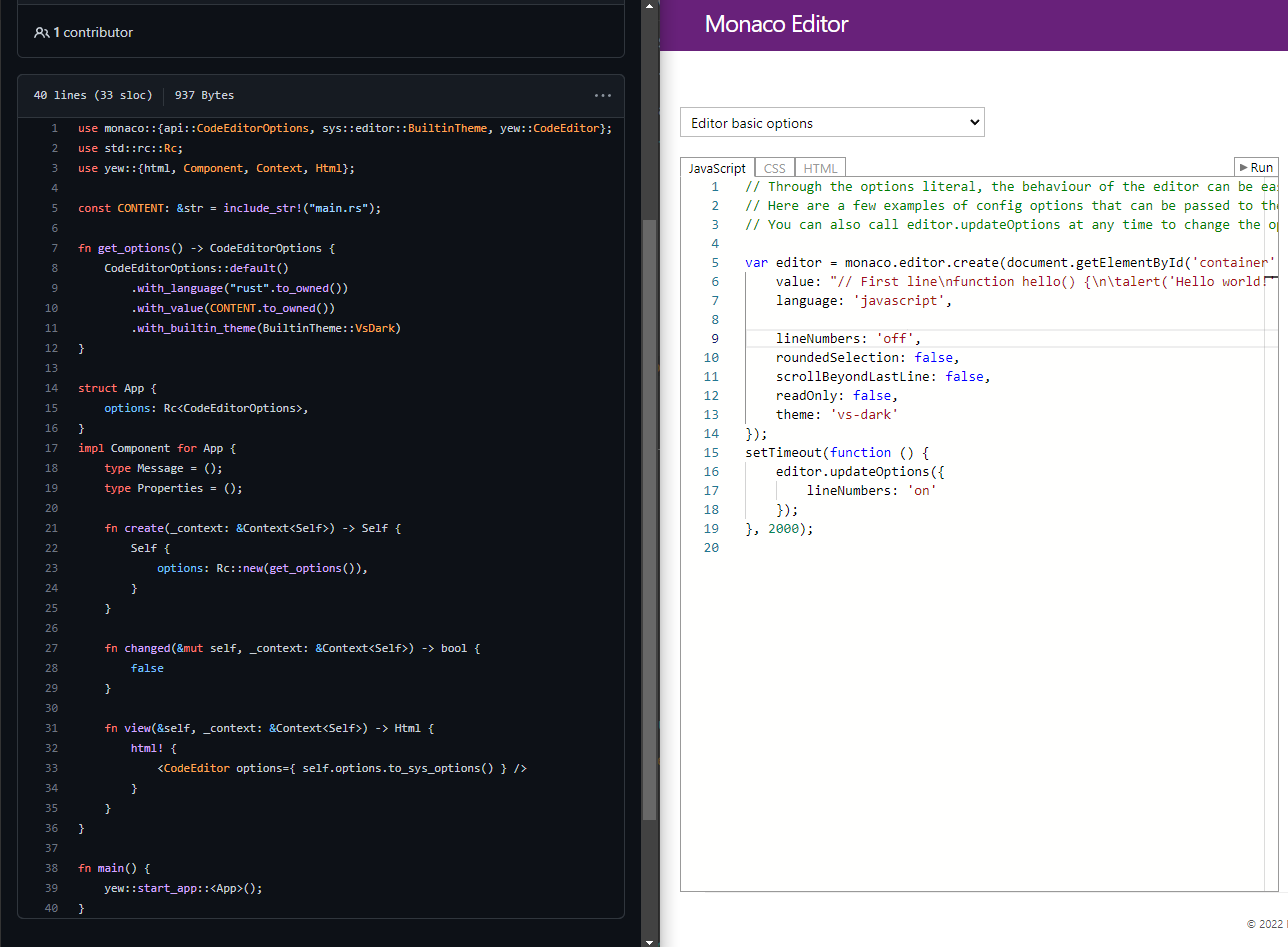
\includegraphics[width=\textwidth]{monaco-initialize}
              \caption{Comparison of initializing the Monaco Editor on Rust(left, rust-monaco) vs. JavaScript(right, Monaco Editor).}
              \label{fig:monaco-initialize}
          \end{figure}

    \item sys -- This is where the bindings for monaco's namespace are located,
          this is how we bind events to the monaco window. An example of this is
          we used IModelDeltaDecoration and IMarkerData to mark where on the
          editor there is an error in the code, which line was previously executed
          by highlighting it, and providing information about the instruction the
          user typed via the hover provider.
    \item workers -- This is required for the performance of Monaco Editor to be
          adequate via web workers, otherwise we get a performance penalty for not
          using it.
    \item yew -- This is for turning the Monaco Editor into a yew component.
\end{itemize}

The sys module is the only one that is optional to use, but the rest are
required (turned on by default) to have it function in Yew.

The crate is an interesting case, because the lead maintainer behind
this used it as proof-of-concept of converting Typescript to Rust with a
Python script then by hand. There was a huge limitation with the crate
and the nature of wasm-bindgen when it came to implementing our custom
language to the application. Trying to implement it properly with
JavaScript, caused the application to crash. This resulted in us forking
over the repository, then replacing the default MIPS language from
Monaco with ours in order for the syntax to highlight properly with some
changes to the regular expressions.

\section{Prototypes}

\subsection{User Interface}

Since one of our main goals for SWIM was to create a visually pleasing
and modern interface for users to easily start working with, one of the
biggest goals on the front end was creating mock-ups and determining how
the interface will look. The prototypes for the graphical front end and
user interface are created by Figma. Figma allowed us to quickly create
a general outline of how our project will look in its final version.

The earliest sketches of the prototype are as follows, showing the basic
functionalities and user interface as well as indicating the locations
of buttons, their functionality, and the layout of the page. Note that
the functionalities buttons are to remain static on the page, some are
made as tabs to switch between data views:

\begin{figure}[H]
    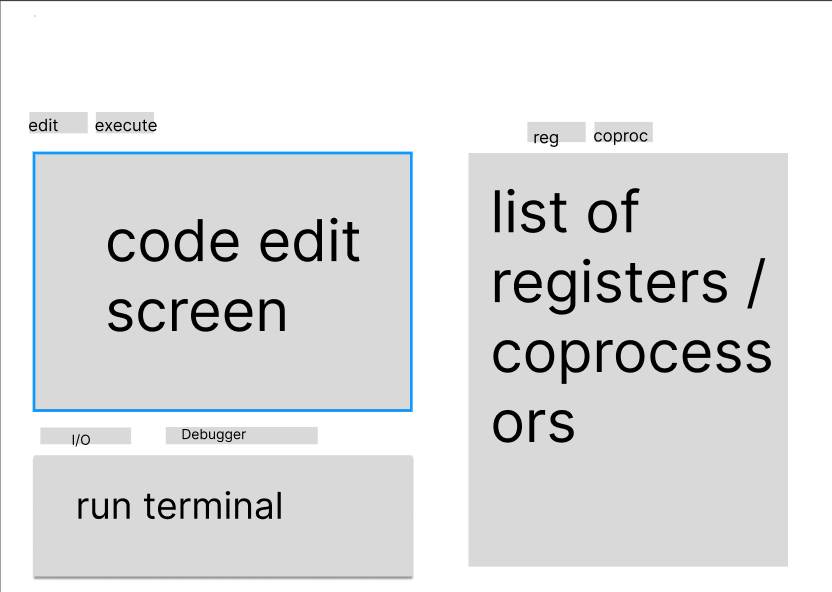
\includegraphics[width=\textwidth]{ui-prototype-1}
    \caption{Layout of UI for SWIM.}
\end{figure}

\begin{figure}[H]
    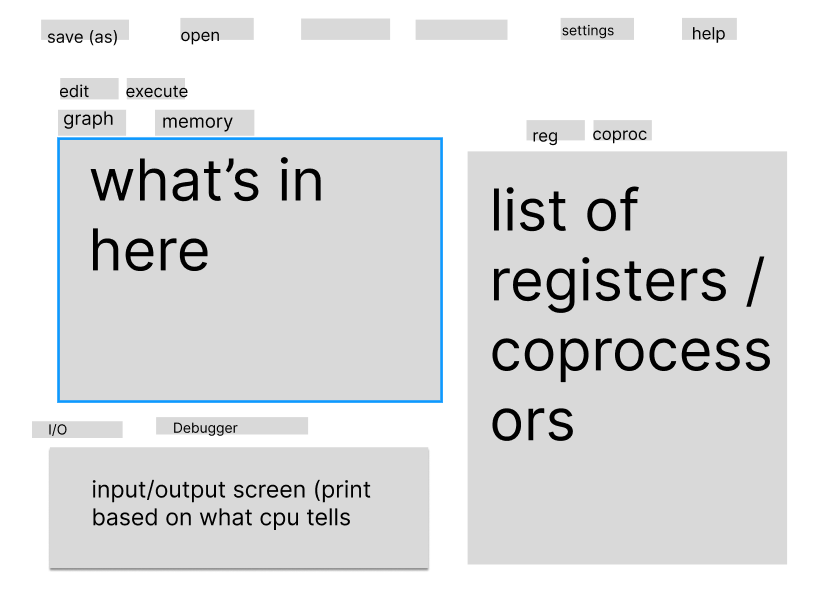
\includegraphics[width=\textwidth]{ui-prototype-2}
    \caption{Layout of UI for SWIM.}
\end{figure}

From this initial design, we further refined the graphical interface. In
this newer iteration, we worked to define button size as well as the
sizes of the various windows of the project. We also sought to get a
general idea of what a possible color scheme could look like on the
project. This interface will be even more refined in the completed
version.

\begin{figure}[H]
    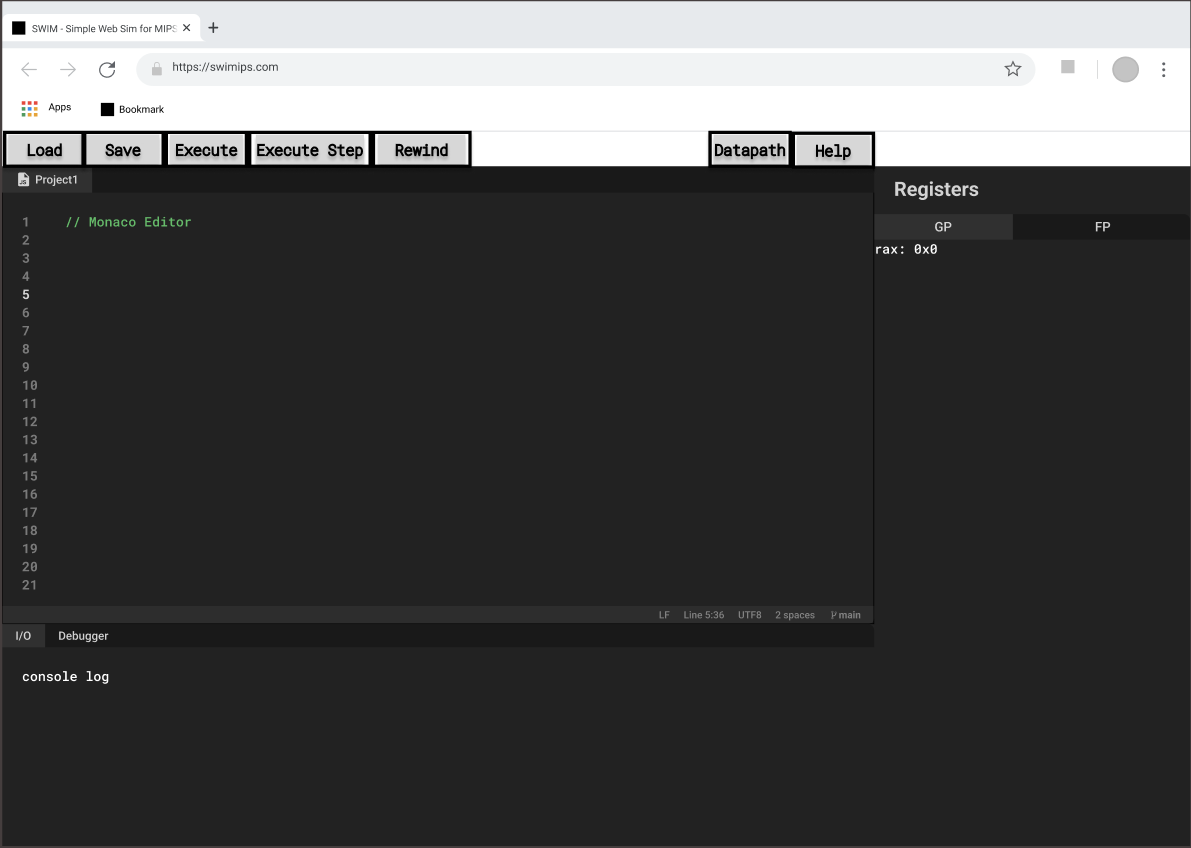
\includegraphics[width=\textwidth]{new-ui-prototype}
    \caption{Layout of UI for SWIM on an example browser, made in Figma, used a code editor mockup in the Figma community for most of the editor, output and register screen layout.}
    \label{fig:new-ui-prototype}
\end{figure}

The prototype indicated by Figure \ref{fig:new-ui-prototype} shows more
clearly the graphical implementation of SWIM, with the main features
like the Monaco Editor, the register view and the console more defined.
The figure does not show more functionalities that we want to implement
or the core functionalities of MIPS (the instructions) as they are core
implementations not meant to be seen by the user. After that prototype
is done, it is a matter of polishing for personalization and
accessibility like color themes, distinction between screens (for
resizing the windows), streamlining the style of buttons, etc. This will
make SWIM fit its name and not look like another Visual Studio Code, or
a worse version of it.

\subsection{Early November Mini Projects}

By the end of October, we had a general idea of our overall approach for
how we were going to build our project. However, most of the technology
we were planning to use were systems that few or none of us had used
before. Even the main programming language of our project, Rust, had
only been used in any serious capacity by a single group member. Along
with that, our actual roles on the project are fairly isolated from each
other. In other words, the implementation of aspects to the graphical
interface has relatively little impact on the way the emulation core or
parser function, for example. To compound this, SWIM is the first time
these group members have worked together on a software project.

Each of those were issues we wanted to address. If we had not used the
technology before, it would be difficult to write extensively about it.
Similarly, we would not know what issues might come up while using those
technologies. Since our roles are so isolated from each other, we wanted
to make sure that each of us knew the scope of our individual roles, as
well as the individual roles of other team members. This understanding
is crucial for the eventual connection of project components between
each of the roles, and to ensure that there is a clear and unified
understanding of the structure and design of the project. Finally, since
none of us have worked together on a project before, there was no
baseline to understanding how our team members work and operate on
software projects and technical tasks. This is especially needed for the
front-end and emulation core roles, where multiple people will be
working in tandem on the same task.

To address all of these issues, we decided to build a series of projects
in the second half of Senior Design I. During the week of October 31st
through November 4th, each team member worked on a small project
individually corresponding to their role on the overall project. Jerrett
and Kevin each worked on creating a small MIPS CPU representation in
Rust, Evan wrote a program in Rust that converted a subset of MIPS
instructions into their binary representation, Jimmie got the Monaco
library in an operational browser demo using the Yew framework, and Huy
built a system to display register values as either hexadecimal or
decimal using the Yew framework.

\subsubsection{Mini Instruction Parser / Assembler - Evan Raiford}

The mini project that I built was a small parser that could read text
files comprised of a small handful of MIPS instructions and comments and
then assembled the instructions as their corresponding binary
representations. This mini project performed the same main task that the
full parser and assembler will do just on a much smaller instruction set
so working on it provided a meaningful glimpse into what I will be doing
on the full project next semester.

The structure of the mini project was fairly simple. It took a .txt file
as input and read its contents into a String and then a for loop
iterated over each of the lines in the String and then printed out the
binary instructions. Since MIPS is an assembly language without the
features of higher level languages like traditional functions or even
variables, most of the work a normal parser needs to take care of is
unnecessary. Each instruction is broken up into a vector of tokens
delimited by the space character. Then, the first element is run through
a match statement to determine what instruction type it is. To keep
things simple for the mini project, the only instructions supported were
\texttt{add}, \texttt{sub}, and \texttt{addi} but the system also was
built to ignore blank lines and comment lines and it also made note of
when an unrecognized instruction was read.

Inside each match case, the binary instruction is built. The first six
bits of the instruction correspond to the instruction type so that
starts the instruction string. Afterward, the destination register is
passed into a function that removes the comma and any extra spaces in
the string and the value is compared in a match statement which returns
the binary value of the register number, between 0 and 31. For
\texttt{add} and \texttt{sub}, this is done twice more to get the other
two vectors in the instruction. The \texttt{shamt} on both is zero and
then the remaining part of the instruction corresponds to what type of
arithmetic is being done so that completes the full instruction which is
then passed back to the main function to be printed out. For
\texttt{addi}, the next step is to read the source register similar to
\texttt{add} and \texttt{sub} but the remaining bits of the binary
instruction are made of the binary for the immediate value being added.
To do this, the String representation of the immediate value is typecast
to being an int and is then translated into binary. However, there are
only 16 bits on the \texttt{addi} function for the immediate value so
the function checks to make sure the value is within the range for a 2's
complement 16 bit integer and notates if it is not. The function also
sign extends positive numbers to be 16 bits long and culls negative
numbers down to 16 bits. The value is then returned back to the previous
function and combined with the other binary to complete the instruction.

Since my mini project was fairly straightforward, I ran into a minimal
amount of issues with building it out. Most of the issues that I did run
into stemmed from my unfamiliarity with Rust. Some of those were minor
like learning Rust does not support do while loops or that its switch
statements are called match statements while others were more
complicated like trying to understand when to use String versus when to
use str and what exactly are the limitations of each.

The mini project provided lots of insights into how I want to structure
the parser and assembler in the full project and helped me figure out
what other things I need to review more and make decisions on. Since the
crux of my role will effectively be just a gigantic match statement, I
want to now try to plan it out to be as readable as possible. It also
helped me realize where my knowledge on MIPS is lacking, for example, on
how MIPS handles an instruction that is broken across multiple lines.

\subsubsection{Register View Decimal to Hex Conversion - Huy Nguyen}

The register view window aims to include labels for data, address, and
stack pointer. The main feature that makes my register view different
from other register view windows is the ability to switch between
hexadecimal and decimal representation of the numbers input through the
data or address. The main function of decimal to hexadecimal conversion,
as well as converting the opposite way, was completed, but the UI looked
nothing like it should. As of early November, the system was not
completed. The mini-project still didn't have the data and MIPS address,
even though the conversion number form was correct. However, when every
functionality is accounted for and made, it will definitely be
incorporated in the main project. What has already been implemented was
the conversion between hexadecimal and decimal values, and a dropdown
list for different kinds of registers. The goal then was to show the
register data when the type is selected.

\begin{figure}[H]
    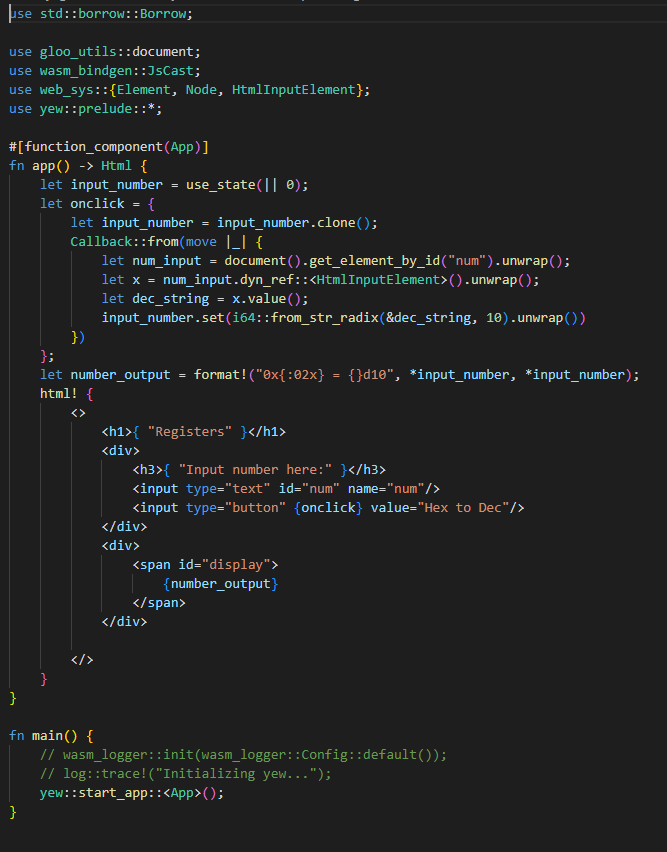
\includegraphics[height=17cm]{huy-register-view-project}
    \caption{main.rs of this register view project. This current code only shows the conversion between hex and decimal values.}
    \label{fig:huy-register-view-project}
\end{figure}

As seen in Figure \ref{fig:huy-register-view-project}, this project uses
dependencies like gloo, wasm-bindgen, HTML websys to be able to use HTML
in Rust and most importantly, Yew. There would be more dependencies used
as the project goes forward, and documentation will become necessary for
those, as well.

There were more challenges to getting this mini-project working than I
expected, with the first being my unfamiliarity with Rust and Yew. Yew
allows for HTML integration, and because of that, I coded like it was
JavaScript and HTML, which caused issues with incorporating with the
example Rust code. I ended up having to use Rust hooks for the
conversions, and it certainly took longer than it should for me to read
through the documents on how to do it. The Rust and Yew documentations
helped with this project, but with how much time I spent for a simple
component, this was going to be a major wall for my progress in the
project.

There was also a problem with API connection. The register window needed
the core to upload the MIPS address and stack pointer so that it can
display data. I was not sure if it could be extracted from within an
operating system of a computer, since MIPS is the base of it. However,
it may not be plausible compared to other ways I could think of, which
shows that I need more understanding on the issue so that this
mini-project goes better and helps the bigger main project.

\subsubsection{Monaco Window - Jimmie Smith}

My mini-project for the project was to get some understanding of how
\texttt{rust-monaco} works. Already, I noticed how different it is to
use Rust as a language to render a webpage compared to JavaScript and it
has been a year since I did anything JavaScript related. I have done a
lot of research on WebAssembly and Yew in order to get an idea of how
Rust is used for front-end development. There is still a lot of ground
to cover since I have to account for documentation for \texttt{web-sys},
Yew, gloo, and \texttt{rust-monaco} for the implementation in Rust with
the addition of \texttt{monaco-editor} and JavaScript APIs as reference.
What I did was looked into the examples provided by Microsoft to see how
the configurations are set up, and they were not too difficult to
understand with the built-in options or configuring how the code would
look with formatting. The difficulty I had with the features is figuring
out what needs to be implemented since this is supposed to be an
educational tool. While I keep on exploring the Monaco Editor's features
and code, I keep a list of features from the team on me to look into.
Implementing Intellisense as a toggle would be challenging since it
would undermine the concepts of the instructions and what they do, so
having the ability to mouse over the instructions the user types and
provide them information on them would be a nice compromise. Monaco
Editor does support MIPS syntax, so it was a matter of toggling it
although the team wanted full support of MIPS32 and MIPS64 which needs
further examination. Monaco Editor has a built-in diff editor, but its
usage for a project like this seems useless for educational purposes.

The best way for me to get an understanding of Monaco and Rust was
through the example code provided with the repository. The first thing
that I was confused by was how the window was not rendered correctly,
the default setting for the window size made it so only a small section
was presented. Jerrett assisted me on remedying the issue, because I was
too used to the documentation being complete for most of the crates and
frameworks. This is where we both learned that rust-monaco's
documentation was not complete which resorted to us looking through the
source code. For example, the documentation does not state that it
supports automatic layout which would let the window scale based on the
current size of the browser window. The hilarity of this is that when we
brought in \texttt{gloo-utils}, it clicked to me why the crate is called
``gloo.'' It is literally taking the idiomatic rust code and converting
it to a web-sys binding which would finally result in JavaScript code to
make the API call. It made me reconsider the whole ecosystem since it is
just a whole bunch of wrappers, but the support for it is plentiful that
it gave me some assurance that this could become an alternative to
developing web applications. From there, it was easy to reconfigure the
settings for the window to read MIPS code. It does auto complete but
based on what was already typed out, and it has a mini preview of the
code on the right by default. An idea I was throwing around is having
line highlights for macro labels for improved readability, so the user
does not have to use block comments to visually break them up.

\begin{figure}[H]
    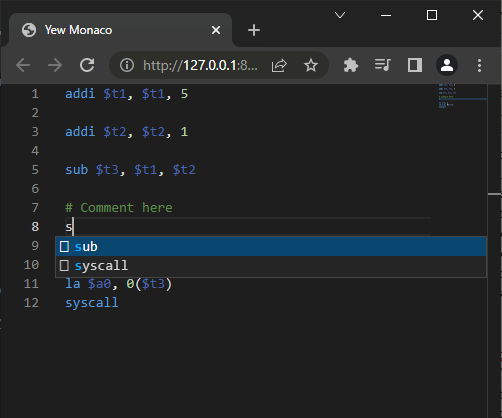
\includegraphics[height=9cm]{jimmie-monaco-prototype}
    \caption{Monaco Window showing MIPS highlighting, auto-complete, code preview, and auto-resizing.}
\end{figure}

\subsubsection{Personal Emulation Core - Kevin Cahalan}

My first major wall with this prototype is that I need to re-familiarize
myself with Rust. It has been over a year since I last had to
professionally develop in Rust. I was not the best at Rust and did not
retain the syntax that well. Use it or lose it, I lost it. Luckily the
principles of Rust exist elsewhere. Since initially learning Rust I have
had to develop and learn Haskell, Go, C++, Swift, TypeScript, and get
massively better at Python. A lot carries over across these languages.
From Swift and TypeScript I got more used to the Rust style of syntax.
Swift in particular held a lot of commonality syntax wise. From Haskell
I picked true functional programming better. Rust takes a lot of
Haskell. I got better with deterministic programming with Haskell. That
deterministic thinking carries over to Rust.

For the first prototype I am doing a simple command line emulator. I am
not even going to worry about web stuff yet. The hope is to support
maybe 15ish mips instructions. These instructions will probably be taken
in as bare binary from a file, or maybe hex from the command line. Gonna
forget about parsing, web stuff, and any real planning. I just want to
get something slapped together and started. After putting together a
bare bones starter emulator my understanding of difficulty and on what
to move onto should become more clear.

For my initial bare bones emulator I started by laying out some
structures. This took a surprisingly long time as I was simultaneously
learning Rust. Particularly I got burned on figuring out how scoping and
modules worked. After some time, and reading the Rust book, I got to the
bottom of things. Finally after so long, I figured out modules to a
usable point. Modules can be thought of as namespaces, probably carried
over from C++ or whatever.

A big part of writing an emulator is to keep track of processor state
and memory. Our simple emulator can be broken down into processor state,
memory, and instructions to change state and memory. MIPS is a simple
Von Neumann Architecture to emulate.

The processor for our project can be thought of as two distinct units,
the Central Processing Unit, and the Floating Processing Unit. The CPU
is the main import unit for doing most basic operations of the
processor. It does all the basic ALU operations, loading, storing, and
so on. Initially in the old days MIPS processors would only have a CPU.
Floating point operations were first implemented in software. As the
years went on, there was a great need for accelerated floating point
calculations. To do these accelerated float pointer operations, MIPS
introduced a new processing unit for their processors, the FPU. A FPU is
a specialized unit used for floating point instructions. Initially these
early FPU's were on a separate chip from the main processing unit, the
CPU. Having the FPU be distinctly separated from the CPU has had a
lasting effect on how floating point operations are done with MIPS.

For laying out the state structures for this emulator, I kept the CPU -
FPU distinction clear. The processor structure both has a CPU struct,
and an FPU struct. Each of these structures then have their own states
to keep track of. I figure that by making this distinction clear, it may
be easier in the future to connect the emulation core to datapath
graphics. We are taking an approach on this emulator less focused on
sense and performance, more-so focused on working like theoretical
hardware. Anyway in Figure \ref{fig:kevin-emulation-core-prototype}
before are my initial processor state structures:

\begin{figure}[H]
    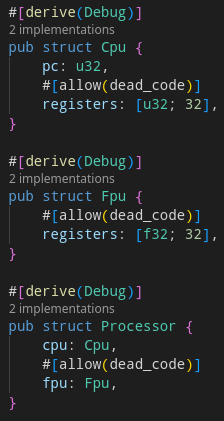
\includegraphics[height=9cm]{kevin-emulation-core-prototype}
    \caption{Processor structure for prototype emulation core.}
    \label{fig:kevin-emulation-core-prototype}
\end{figure}

The processor structure is, to some extent, simple. It got the basic
general purpose register, floating point registers, and the instruction
pointer PC. There are likely several other state registers that I will
have to add in the future. For now this processor structure is good
enough to move on.

My general emulation core is all under some structure called
\texttt{Emulator}. So far this struct just holds the memory array and
processor struct. Glued to the Emulator struct are some basic methods
for emulation and access to the emulation core. To interact with the
emulation core, the front end will call a set of public methods that the
emulation core implements. Currently the only public method that I have
made is called \texttt{run\_instruction()}. This method will exactly as
stated, step forward running one instruction. Underneath the protection
of the emu module are the private methods for actually doing the hard
work of emulation. I am going with the heavy encapsulation on this
emulation core. The front-end developers should not have to worry about
any of the details of emulation core implementation.

\section{Implementation Overview}

SWIM uses a collection of three components to complete the full
functionality of the project: an emulation core, a parser, and an
interface / front end. Each of these components are each explained in
more detail in Sections \ref{sec:emulation-core}, \ref{sec:parser}, and
\ref{sec:front-end}, respectively. In a pictorial representation,
Figures \ref{fig:use-case-diagram} and \ref{fig:block-diagram} show the
layout and usage of these components.

\subsection{Use Case Diagram}

\begin{figure}[H]
    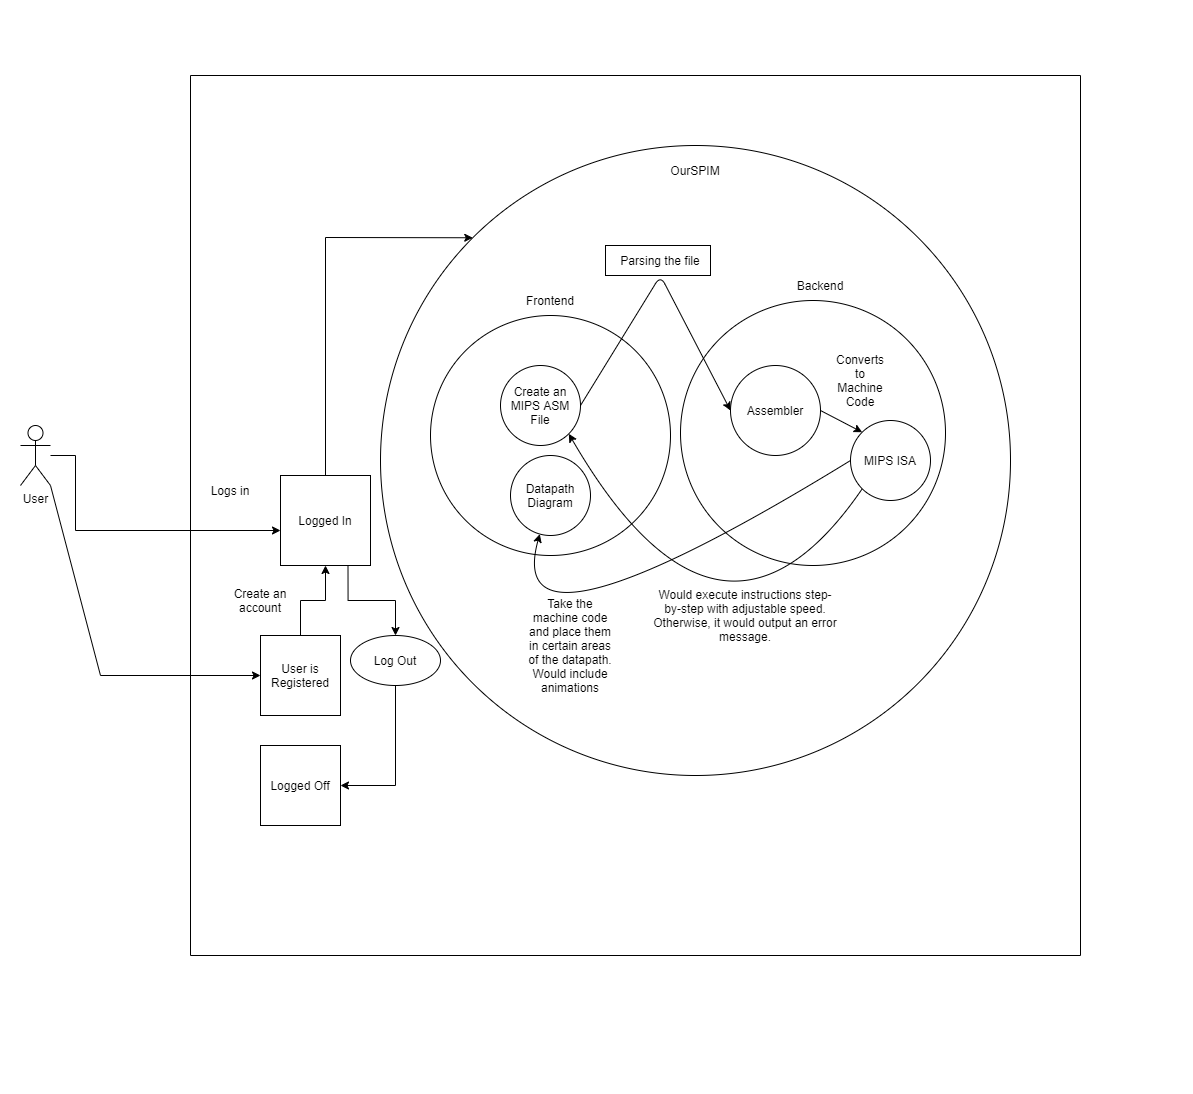
\includegraphics[width=\textwidth]{use-case-diagram}
    \caption{Use case diagram of SWIM.}
    \label{fig:use-case-diagram}
\end{figure}

\subsection{Block Diagram}

\begin{figure}[H]
    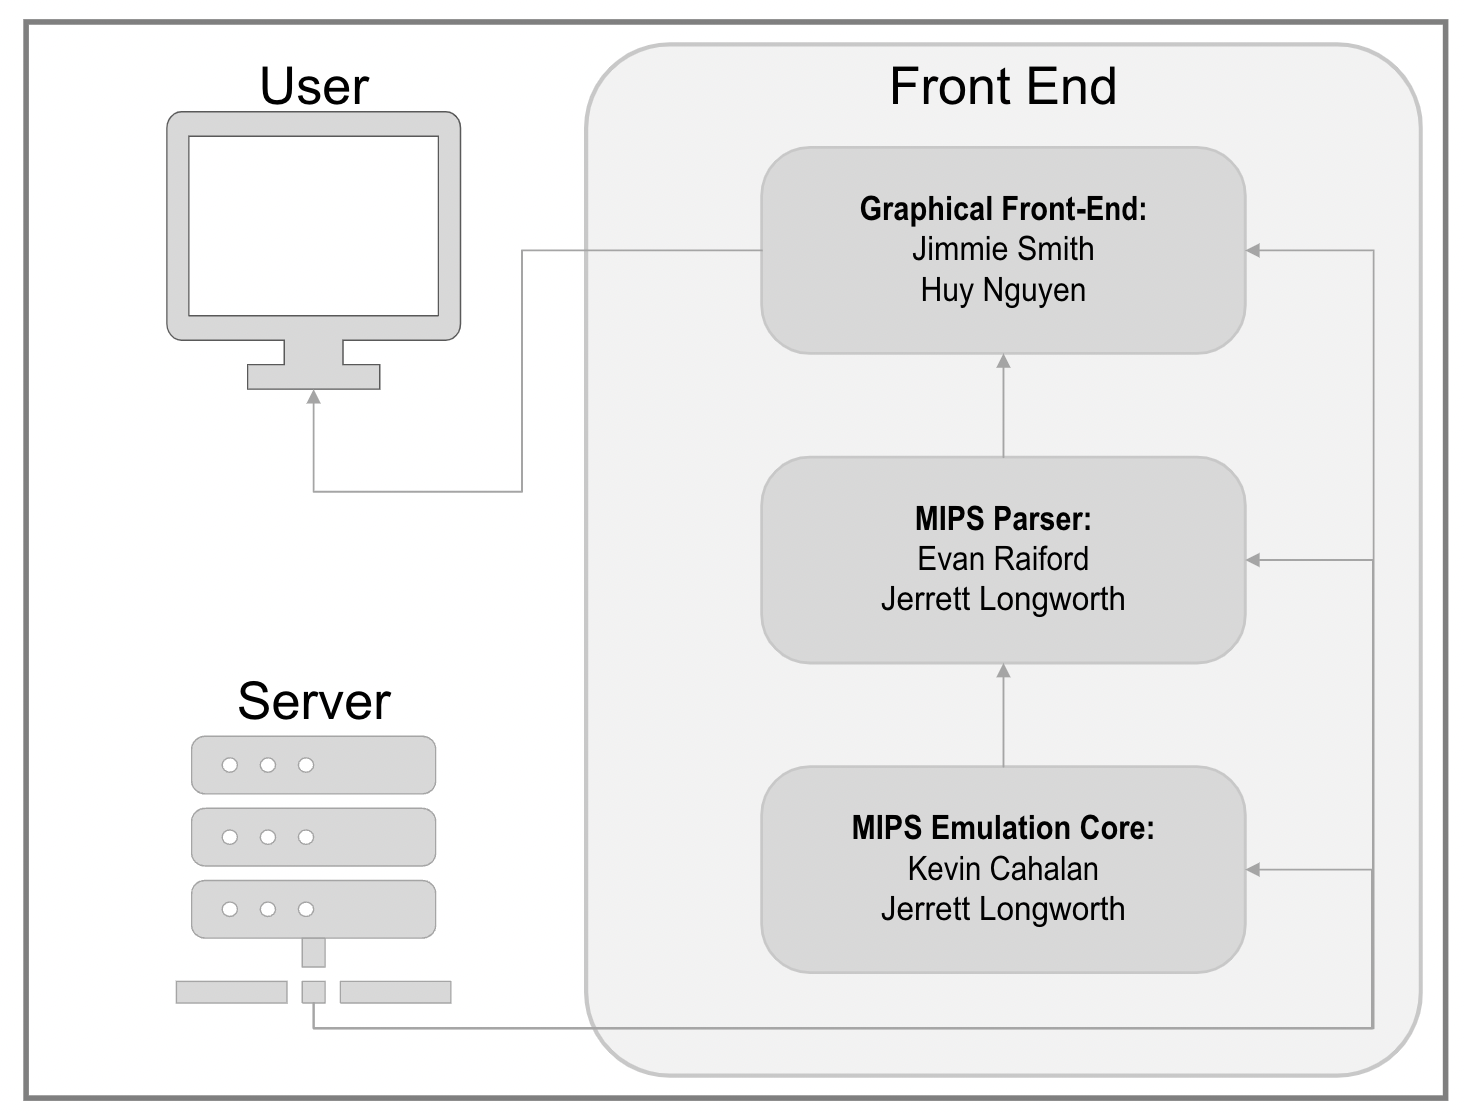
\includegraphics[width=\textwidth]{block-diagram}
    \caption{Block diagram of SWIM.}
    \label{fig:block-diagram}
\end{figure}

\section{Pseudo-Single-Cycle Datapath Implementation}
\label{sec:emulation-core}

Our implementation of a MIPS single-cycle datapath, also referred to
throughout this document as the ``emulation core,'' is designed to be
easy to use as both a developer and an end user. Throughout the
development of the emulation core, its design is influenced by the
visual datapath feature in SWIM.

\subsection{Approach and Reasoning}

The datapath is structured to mimic a single-cycle datapath out of a few
considerations in the project design. A pipelined datapath, while more
efficient in real-world situations, can be more complex for students to
learn just beginning a computer architecture and design course. In
addition, instruction-level parallelism introduces additional
programming complexity that is not feasible for a first release of this
project. With the use of a pipelined datapath, there comes a large swath
of additional technical considerations, such as handling hazards and the
use of branch prediction.

However, while the pipeline itself and parallelism is not implemented,
the emulation core is structured in a way that modularizes each stage of
the datapath, such that pipelining would be easier to add at a future
point. Each of the five stages in the datapath (Instruction Fetch,
Instruction Decode, Execute, Memory, Writeback) is split in source code
for the purpose of this future implementation. In a real-world
implementation, a CPU designed with stages but without pipelining would
be inefficient and less performant than, for example, using a
single-cycle or multi-cycle datapath. However, for the previously
mentioned reasons, we have considered this acceptable for this project.

Beyond pipelining, SWIM allows users to execute instructions one stage
at a time. Users can additionally view a visual representation of
instructions passing through a datapath. (See Section
\ref{subsec:datapath-visual-representation} for more details.) These
features combine to view individual instructions passing through the
datapath at a more granular level, as if it were pipelined.

\subsection{Approaches of Representing Instructions}

In our project, we take two levels of abstractions for how instructions
are handled inside the emulation core. One level of instruction handling
is with integer values for each instruction and each field. In a basic
sense, a MIPS64 instruction is just a 32-bit integer value, thus when
referring to a specific field from an instruction, additional variables
can shift and clear bits as needed.

However, handing instructions as simple integer values may not be
appropriate for all development cases. For instance, using repetitive
bit masking and isolation is error-prone and reduces code readability.
In the MIPS64 specification, different instructions use varying names to
describe fields with varying widths. As an example, R-type instructions
use \texttt{op}, \texttt{rs}, \texttt{rt}, \texttt{rd}, \texttt{shamt},
and \texttt{funct}, whereas FPU R-type instructions use \texttt{op},
\texttt{fmt}, \texttt{ft}, \texttt{fs}, \texttt{fd}, and
\texttt{function}. These instruction types may use the same field
widths, however use completely different names to describe them. Using
integer values throughout the emulation core can cause confusion for
developers as fields are re-used with differing names, depending on the
context. The key to avoid this is with a second level of abstraction.
This abstraction, specific to this project, takes advantage of Rust's
ability to use enums and structs.

While the second level of abstraction is used for handling instruction
fields throughout the emulation core, the first level remains
appropriate for the visual datapath feature, as this feature
necessitates decribing and viewing each individual wire in the datapath.

This dual instruction handling, while first appearing to be redundant,
has been effective for this project. Adding new instruction formats and
behavior in practice has been easy with the second added level of
abstraction. The first level of abstraction remains appropriate for
working in tandem with individual wires in the datapath.

\subsection{Supported Instructions}
\label{subsec:supported-instructions}

The following table is an all-inclusive list of the assembly
instructions supported in SWIM.

\begin{itemize}
    \tightlist
    \item Instructions marked with an asterisk (*) follow the MIPS Release 5
          specification, while unmarked instructions follow the MIPS Release 6
          specification.
    \item Instructions marked with a plus (\textsuperscript{+}) are
          pseudo-instructions, but are grouped in a different category for
          organization.
\end{itemize}

{\renewcommand{\arraystretch}{1.4}
\begin{tabularx}{\textwidth}{|L|L|L|L|L|L|}
    \hline
    \multicolumn{6}{|l|}{\emph{\ul{Arithmetic and Immediate Instructions:}}}                                                                                                                                                                                    \\ \hline
    add                                               & sub                        & mul                       & div                                          & or                                                     & and                                    \\ \hline
    addi*                                             & subi\textsuperscript{+}    & muli\textsuperscript{+}   & divi\textsuperscript{+}                      & ori (or immediate)                                     & andi                                   \\ \hline
    seq\textsuperscript{+} (set equal)                & sne\textsuperscript{+} (≠) & slt (\textless)           & sle\textsuperscript{+} (\textless=)          & sgt\textsuperscript{+} (\textgreater)                  & sge\textsuperscript{+} (\textgreater=) \\ \hline
                                                      &                            & sltu                      & sleu\textsuperscript{+}                      & sgtu\textsuperscript{+}                                & sgeu\textsuperscript{+}                \\ \hline
    lui (load upper immediate)                        &                            &                           &                                              &                                                        &                                        \\ \hline
    \multicolumn{6}{|l|}{\emph{\ul{Arithmetic and Immediate Instructions (MIPS64):}}}                                                                                                                                                                           \\ \hline
    dadd (add 64-bit integers)                        & dsub                       & dmul                      & ddiv                                         & dahi (double-word add high immediate)                  & dati (double-word add top immediate)   \\ \hline
    daddi*                                            & dsubi\textsuperscript{+}   & dmuli\textsuperscript{+}  & ddivi\textsuperscript{+}                     &                                                        &                                        \\ \hline
    daddiu                                            & dsubiu\textsuperscript{+}  & dmuliu\textsuperscript{+} & ddiviu\textsuperscript{+}                    &                                                        &                                        \\ \hline
    \multicolumn{6}{|l|}{\emph{\ul{Floating-Point Instructions (MIPS64):}}}                                                                                                                                                                                     \\ \hline
    mtc1 (move to coprocessor 1)                      & dmtc1 (double move)        & mfc1                      & dmfc1                                        &                                                        &                                        \\ \hline
    add.s                                             & sub.s                      & mul.s                     & div.s                                        &                                                        &                                        \\ \hline
    add.d                                             & sub.d                      & mul.d                     & div.d                                        &                                                        &                                        \\ \hline
    c.eq.s* (compare if equal single-precision float) & c.lt.s* (\textless)        & c.le.s* (\textless=)      & c.ngt.s* (! \textgreater) (not greater than) & c.nge.s* (! \textgreater=) (not greater than or equal) &                                        \\ \hline
    c.eq.d*                                           & c.lt.d*                    & c.le.d*                   & c.ngt.d*                                     & c.nge.d*                                               &                                        \\ \hline
    \multicolumn{6}{|l|}{\emph{\ul{Branch Instructions:}}}                                                                                                                                                                                                      \\ \hline
    j                                                 &                            &                           & beq                                          & bne                                                    &                                        \\ \hline
    \multicolumn{6}{|l|}{\emph{\ul{Pseudo-Instructions:}}}                                                                                                                                                                                                      \\ \hline
    li                                                &                            &                           &                                              &                                                        &                                        \\ \hline
    \multicolumn{6}{|l|}{\emph{\ul{Memory Instructions:}}}                                                                                                                                                                                                      \\ \hline
    lw                                                & sw                         &                           &                                              &                                                        &                                        \\ \hline
    lwc1 (load word to coprocessor 1)                 & swc1                       &                           &                                              &                                                        &                                        \\ \hline
\end{tabularx}}

For the simplicity of usage, some instructions have been brought from
the MIPS Release 5 specification, causing some conflicts with
instructions in the MIPS Release 6 specification. While none of the
supported instructions are affected by this mix of specification, it
should be noted that the following MIPS Release 6 instructions are
directly incompatible with the supported instruction list:

\begin{itemize}
    \tightlist
    \item From \texttt{addi}: \texttt{beqzalc}, \texttt{bnezalc}, \texttt{beqc},
          and \texttt{bovc}
    \item From \texttt{c.cond.fmt}: \texttt{cmp.condn.fmt}
\end{itemize}

In addition, we partially support the \texttt{syscall} instruction as a
way to end a program. Since true I/O or exceptions are not within the
scope of a first release, we have decided to designate the
\texttt{syscall} instruction essentially as the ``stop'' instruction,
which halts the emulation core. This instruction is expected to indicate
to the overall SWIM interface that a program has ended, either
intentionally or not. (The emulation core will likewise halt in the
event of an invalid instruction.)

\subsection{Full Datapath}

\begin{figure}[H]
    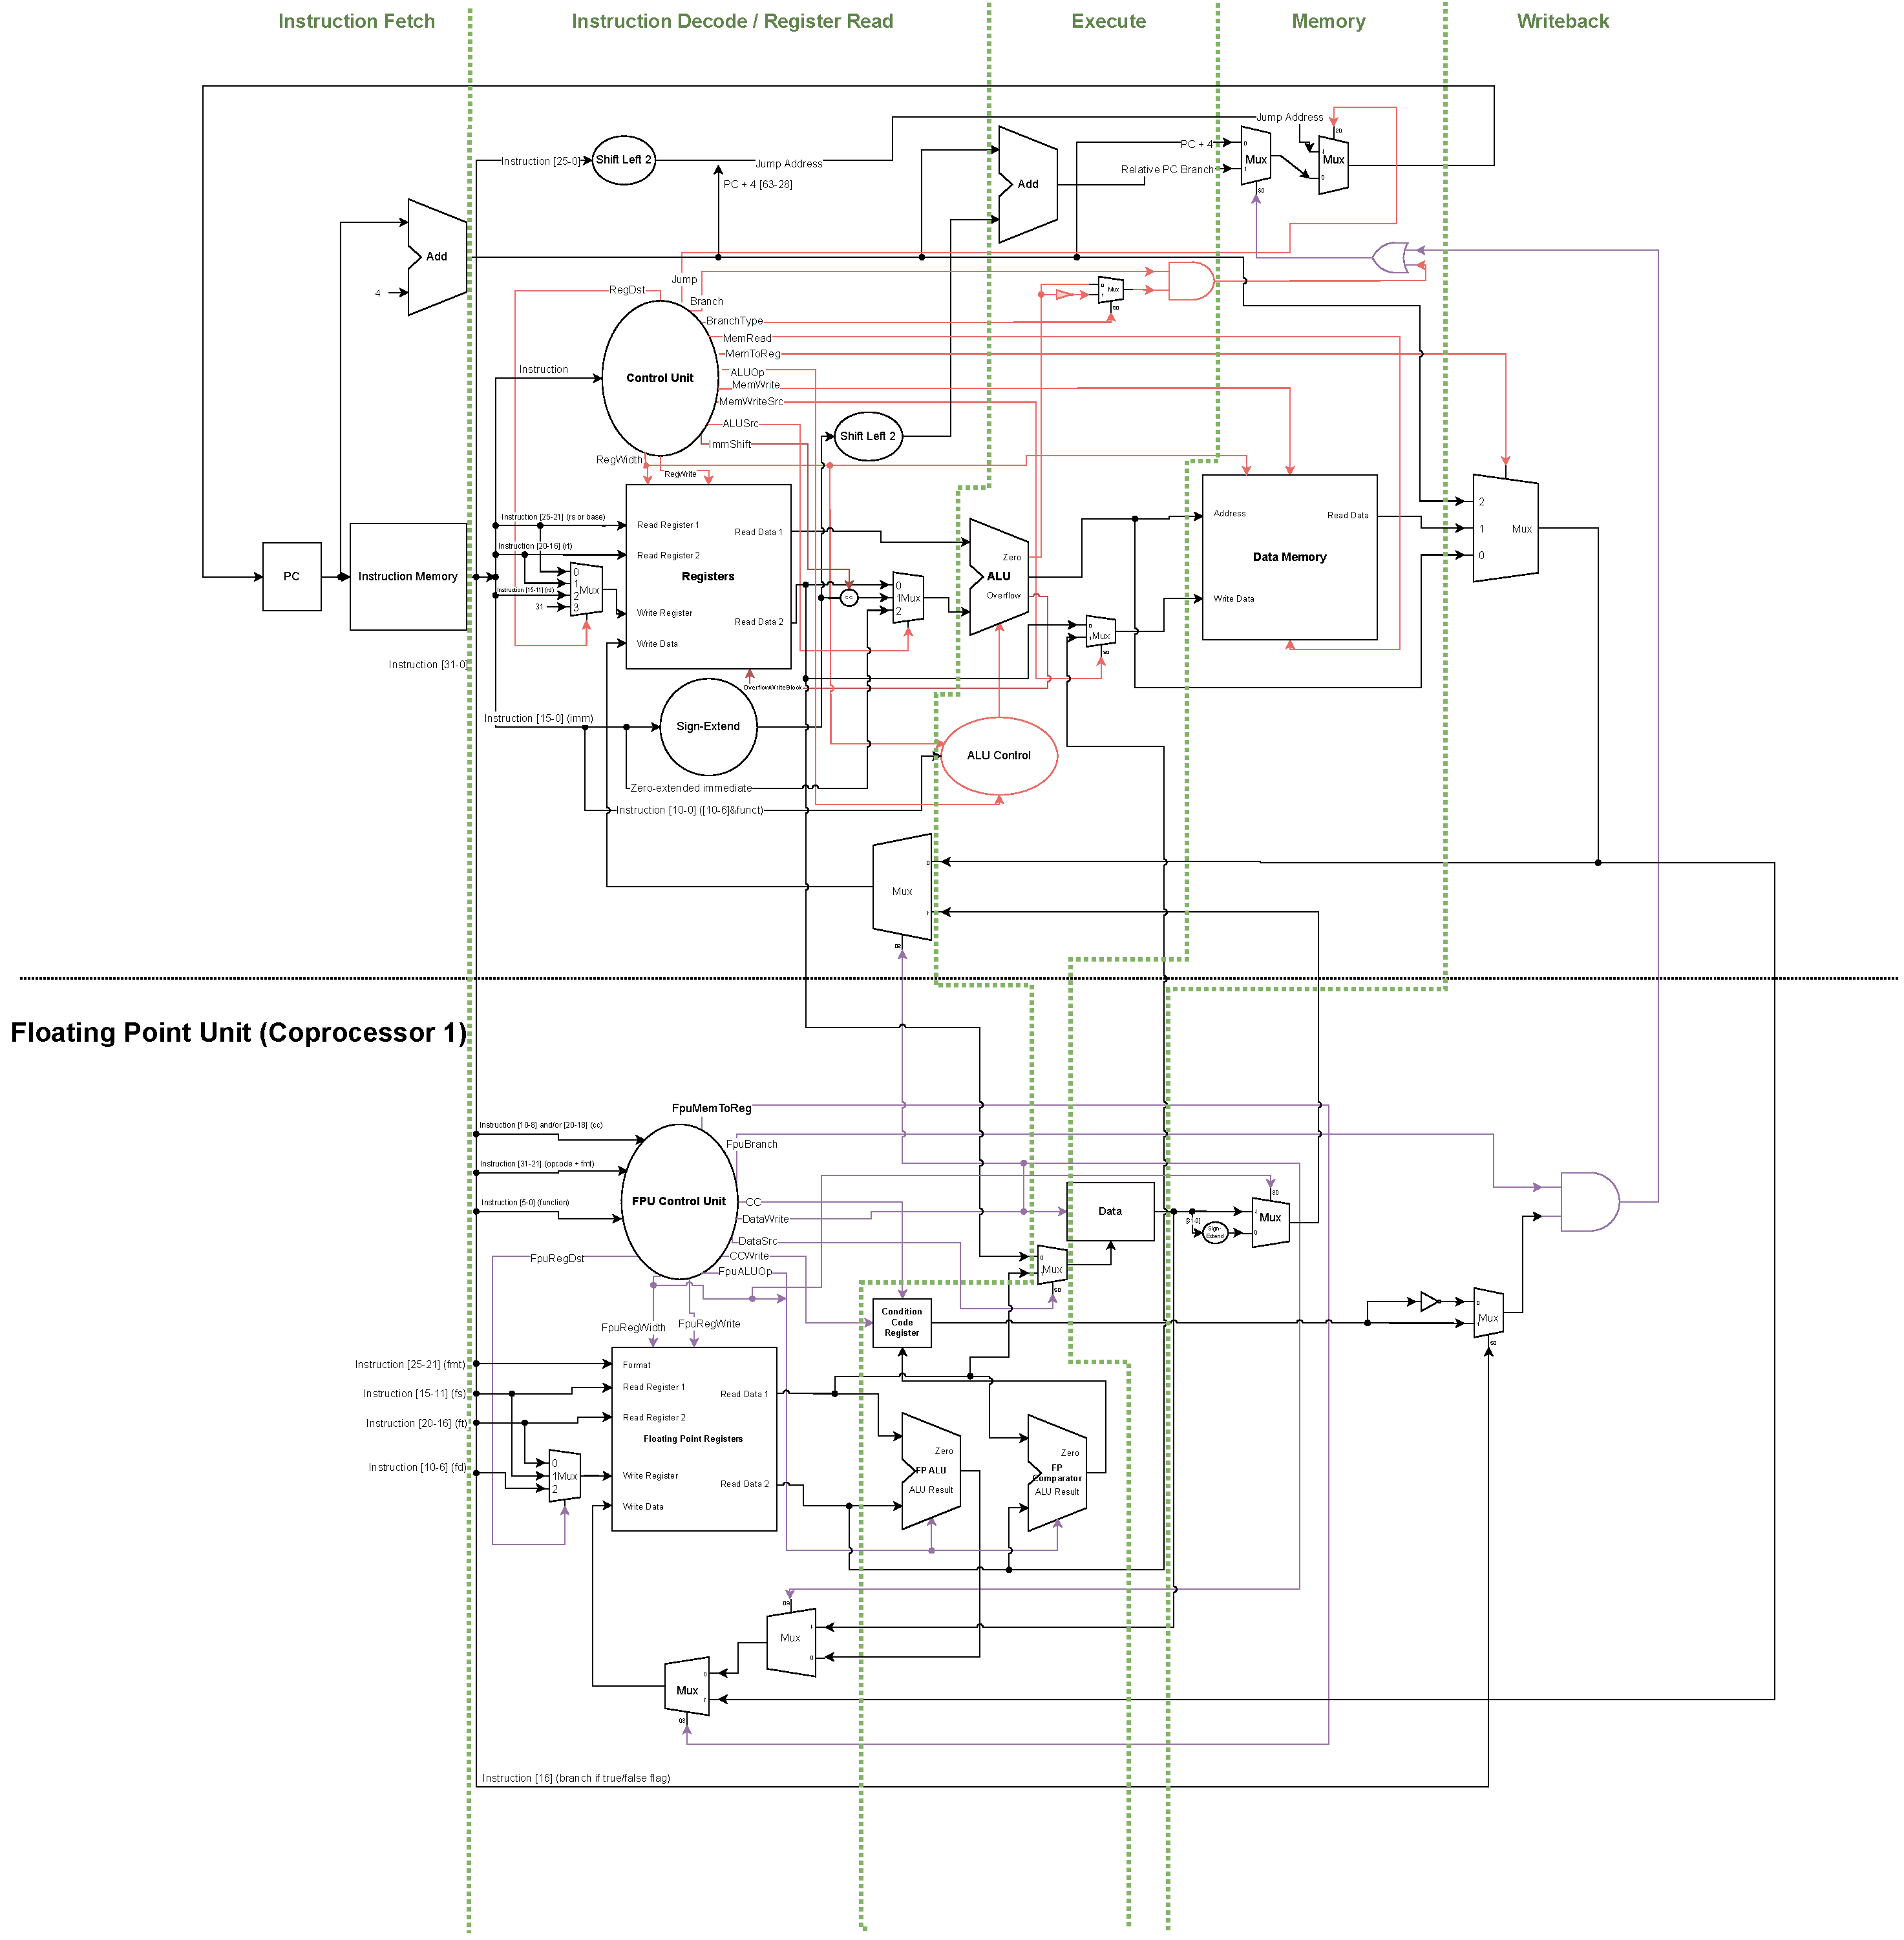
\includegraphics[width=\textwidth]{swim-datapath}
    \caption{Full simulated datapath including the floating-point unit. Red lines represent primary processor control signals. Purple lines represent floating-point unit control signals.}
\end{figure}

The simulated datapath used for this project's emulation core can be
considered to be an extension of the datapath by Hennessy and Patterson
in their textbook \cite{hennessy-patterson}. This datapath was chosen as
a basis for our own datapath to the benefit of students already familiar
with the layout. While it offers support for many of the instructions
from the MIPS32 instruction set, including many of the standard
arithmetic, branch, and jump instructions, it lacks support for MIPS64
instructions and any floating-point operations. To add this additional
functionality, an original floating point unit was added into the
datapath and new control signals were added to the existing control
unit.

In the main processing unit, two signals were added to the control unit
to support the extended instruction set: RegWidth and MemWriteSrc. These
control signals determine the effective size of the registers and the
source of data to write to memory from, respectively. With regard to
RegWidth, it was a priority to use the existing data lines to reduce
complexity, and to accomplish this, almost all 32-bit lines are
converted to 64-bit lines. This maintains compatibility with any 32-bit
instructions and data by having the register file, ALU, and memory unit
simply agreeing to only consider the lower 32-bits of the data.
Depending on the location of the datapath and its implementation, the
other discarded bits may be considered zero or uninitialized values.

When designing the floating-point unit, an emphasis was made to make it
similar in structure to the primary computation unit to give an easier
understanding to new viewers, as floating-point functionality is not
always modeled in datapaths for computer architecture courses. This
floating-point unit offers a similar structure, with registers on the
left, a control unit above them, and ALUs to the right. Many of the same
control signals carry over with similar features, such as FpuMemToReg,
FpuBranch, and FpuRegWrite. The general rule-of-thumb used for this
design process was to become incrementally more complex for each new
case that was added. For instance, the initial datapath for the
floating-point unit could be considered almost identical to its primary
unit counterpart's ID and EX stages. On a broad level, for each slightly
more complex feature, either a new line was created or an existing line
was split, with the possible addition of a new logic unit. Going from a
single floating-point ALU to including an additional floating-point
comparator is one such example.

When incorporating the functionality specific to the floating-point
unit, the most notable in original structure is this inclusion of a
separate comparator, as well as a condition code register. The
functionality for this was designed to mirror how the existing
floating-point ALU operates: The comparator has two inputs from
registers, performs an operation, and writes the data to a special
condition code register. This condition code register has a control
signal for write permission and a control signal for selecting which
condition code register to use (though for this project, it is assumed
that the first condition code register will always be used).

One of the last incremental changes to the datapath as a whole was the
functionality to transfer data between the main processor and the
floating-point unit. Many existing lines must be split or multiplexed,
but are done so in a way that extends existing functionality. The
general nomenclature used for any new control signals (like DataWrite,
FpuBranch, and MemWriteSrc) was that zero represents a ``disabled'' or
``default'' state, implying that setting these new control signals to
zero, effectively ignoring them, would restore the original
functionality of the datapath by Henessy and Patterson.

\subsection{ALU}

Most CPU instructions revolve around the use of arithmetic operations.
Everything from simple register manipulation, to loading and storing,
would all end up needing some kind of arithmetic or logic operation. ALU
stands for ``arithmetic logic unit,'' and can perform addition,
subtraction, bitwise logic, and several kinds of checks. ALUs are
dynamic, having at runtime their operations specified with some kind of
operation code. There is no standard for operation codes in practice.

% TODO: Source for these operations being used in MIPS education?
The simple ALU generally used in MIPS education (when discussing
specifically its implementation) supports eight operations, taking a
3-bit operation code. However, this is limited in ability, as many
instructions that SWIM requires cannot be supported with only eight ALU
operations. The eight-operation ALU can perform the following
operations: \emph{add}, \emph{subtract}, \emph{unsigned compare},
\emph{signed compare}, \emph{bitwise and}, \emph{bitwise or}, \emph{left
    shift 16}, and \emph{bitwise not}. Operations such as \emph{multiply},
\emph{xor}, and so on, are missing. For this project, as outlined by the
control signals in Section \ref{subsec:control-signals}, we use an
extended version of the simple eight-operation ALU, where the operation
code has been expanded to four bits, allowing for 16 total operations.
The original eight are preserved, as those are commonly used in
education, and additional operations follow after.

For the sake of this project, only one ALU is required in the primary
unit, and an additional floating-point ALU is required in the
floating-point unit.

\subsubsection{ALU Control Unit}

An ALU control unit is the component of a processor that selects the
operations for an ALU, playing a role in the Instruction Decode stage.
In the standard single-cycle MIPS datapath, there is a single ALU
control unit that effectively maps R-type function bits to ALU operation
codes. See Section \ref{subsec:control-signals} for details on the
implementation of ALU control unit signals.

\subsection{Register File}

\underline{\textbf{Implementation in Rust:}}
\begin{verbatim}
#[derive(Clone, Copy, Default, PartialEq)]
    pub struct Registers {
    pub pc: u64,
    pub gpr: [u64; 32],
}
\end{verbatim}

The register file is organized and implemented in a way that is both
easy to develop with and is faithful to how registers may be organized
in a real-world datapath. In the context of development, it is
especially important that interfacing with the registers is flexible,
since they are directly accessed in both the front end and the emulation
core.

Notice that all registers are stored as unsigned 64-bit integers. While
the types of data stored in these registers can vary, the motivation for
this decision stems from the idea of interfacing with these registers.
By having a common data type between all of these registers, this allows
any APIs for the Register struct to use the same data types, both for
reading and writing. Variations in data types, including 32-bit integers
and floating-point values, are handled by some form of casting within
Rust. In implementation, integers can easily be cast between 32-bit and
64-bit variations. For the case of converting to or from floating-point
values, they do not correlate in binary, so a function from Rust's
standard library instead handles this. (\texttt{f64::to\_bits()} and
\texttt{f64::from\_bits()}, for example.)

In order to make development with registers simple but flexible, there
are three ways to access individual registers, with these variations
becoming useful based on the multiple contexts in which registers are
used. The first (and most straight-forward) method of accessing
registers is to simply access individual members within the Registers
struct. For example, to access the \$zero register, one may use
\texttt{datapath.registers.gpr[0]}. This method is built into the Rust
language and is ideal for situations that involve work internally within
the datapath. To illustrate, extracted register fields from an R-type
instruction can easily be passed into the index of an array of
general-purpose registers. It is assumed that a developer programming
within the datapath will be using valid array indices, and Rust will by
default panic, should an invalid index be used, which is as intended.

The second and third methods of accessing registers involve indexing the
struct as a whole, rather than out of elements of an array. This is
possible due to the Index and IndexMut traits available in Rust. For
example, a programmer could write \texttt{datapath.registers[\textless
            register\textgreater]}, with a specification of the register within the
square brackets. This method of indexing was created out of a desire to
keep the API between elements of the datapath and the interface as
simple as possible. While the interface does still have access to
individual members of the struct, it can consider the Register struct as
a whole more generally. The sole difference between the Index and
IndexMut traits is that the Index trait handles cases where non-mutable
instances are requested, and the IndexMut trait handles cases where
mutable instances are requested. For example, consider the difference
between the assignments \texttt{x = datapath.registers[r]} versus
\texttt{datapath.registers[r] = x}. Only one of these scenarios requires
a mutable reference.

In terms of how the Index and IndexMut traits are used, the first method
is to index by a newly-created RegisterType enum. The RegisterType enum
simply lists all the valid registers implemented for this datapath. This
mandates that a valid register is accessed. For example, register \$t1
(the tenth general-purpose register) can be accessed by
\texttt{datapath.registers[RegisterType::T1]}. While more verbose, this
makes visibility and understanding within code for development easier.
The purpose of this indexing method is mainly for creating tests, as
registers become easily identifiable, while also safe within Rust's
static code checking.

The third method of indexing (and the second method taking advantage of
the Index and IndexMut traits) is by string. For example, register \$sp
(the thirtieth general-purpose register) can be accessed by
\texttt{datapath.registers["sp"]}. This is by far the most simplistic in
terms of its readability, and is intended for use within the front end.
For the case where the user desires to access a register by providing
its name manually, this is easily possible using this method. While it
is possible to give an invalid register name, it is simple to use from a
programming perspective.

One data type not implemented with the Index and IndexMut traits is any
form of integer (e.g. u32, i32, usize). It was decided that this would
be conducive to non-standard nomenclature for the MIPS ISA, against the
primary goal of the project to be easy to use in educational
environments. For example, the 32 general-purpose registers could easily
map to indices 0 through 31, but leaves for debate the indices to be
used for the program counter and floating-point registers. All such
decisions would be nomenclature original to the project that would only
act to confuse others.

To assist with the implementation of register indexing, we used the
crate \texttt{strum} \cite{strum}, which provides mappings between
strings and enums. This allows implementing SWIM to access registers
with a string or an enum easily with the addition of a new
\texttt{EnumString} macro.

An additional method of interfacing with the Registers struct is to
additionally implement the \texttt{Iterator} and \texttt{IntoIterator}
traits for iteration. This further allows for simple access with
registers by allowing a front-end programmer to essentially use
\texttt{for register in registers} in displaying the contents of all
registers.

\subsubsection{Floating-Point Register File}

Notably absent from the register-file are floating-point registers. Due
to the rules surrounding Rust's ownership system, it was determined that
the simplest way to implement registers in the floating-point
coprocessor was to add them as fields to the coprocessor data structure
itself.

\underline{\textbf{Floating-Point Coprocessor Implementation in Rust:}}
\begin{verbatim}
#[derive(Clone, Default, PartialEq)]
pub struct MipsFpCoprocessor {
    instruction: Instruction,
    pub signals: FpuControlSignals,
    pub state: FpuState,
    pub is_halted: bool,

    pub fpr: [u64; 32],
    pub condition_code: u64,
    data: u64,
}
\end{verbatim}

A notable (but reasonable) departure has been made from the standard
MIPS64 specification surrounding the \texttt{condition\_code} register
that resides on the floating-point unit. Within the MIPS specification,
an instruction may include multiple bits to indicate a selection of
multiple condition code registers. However, for all intents and purposes
in this project, this specific aspect of the datapath reflects MIPS
Release 5, not the latest Release 6 as of the time of writing. Any other
condition code registers are not considered in any of the supported
instructions for this implementation of the datapath.

\subsection{Data and Instruction Memory}

\underline{\textbf{Implementation in Rust:}}
\begin{verbatim}
const CAPACITY_BYTES: usize = 64 * 1024;
pub struct Memory {
    pub memory: Vec<u8>,
}

impl Default for Memory {
    fn default() -> Self {
        Self {
            memory: vec![0; CAPACITY_BYTES],
        }
    }
}
\end{verbatim}

We have created our memory in the form of a vector of individual bytes,
which allows it to stand on its own as an extensible medium for loading
and storing data. A struct is used to allow associated methods and
properties, compared to simply a standalone vector. Memory is
byte-addressable if needed, but it will be more common to request data
from memory by word or by double word. Functions have been built into
the Memory struct to translate between contiguous bytes within a vector
and 32-bit and 64-bit values. Internal functions such as
\texttt{load\_word()} and \texttt{store\_double\_word()} make this
process simple for interfacing in a wide range of data types. We have
decided to use 64 KB of storage for this memory at this time.

\subsubsection{Endianness}

The MIPS specification allows for both little-endian and big-endian
formats, so the choice for which endianness system to use is completely
at our discretion. We have decided to store data in memory and registers
in a big-endian format. This means that the most significant bit of a
number at the lowest address it is in. For example, the value 5:

\begin{tabularx}{\textwidth}{|l|c|c|c|c|}
    \hline
    \textbf{Bits:}    & 00000000 & 00000000 & 00000000 & 00000101 \\\hline
    \textbf{Address:} & 0x5000   & 0x5001   & 0x5002   & 0x5003   \\\hline
\end{tabularx}

The reason for this is that Western nomenclature for numbers tends to
prefer a big-endian format. In \cite{hennessy-patterson}, binary numbers
are written in big-endian for most if not all examples, so this system
is mirrored in SWIM.

\subsection{Control Signals}
\label{subsec:control-signals}

The following control signals are used in the standard integer portion
of the datapath, and described are their roles and possible values.
These control signals are largely based on those from Hennessy and
Patterson \cite{hennessy-patterson}, in order to be familiar for
students using SWIM for their courses.

\begin{itemize}
    \item ALUControl
          \begin{itemize}
              \tightlist
              \item The output of the ALU control unit that directly controls the ALU. This
                    is not to be confused with the ALUOp signal. ALUControl is a function of
                    both ALUOp and the ``funct'' field of an R-type instruction. The leading
                    bit of this signal determines the size of the input and output data. If
                    this bit is 0, it indicates an operation using words (32-bits). If this
                    bit is 1, it indicates an operation using doublewords (64-bits). This
                    leading bit is determined by the RegWidth control signal.
              \item \_ 0000 (0) - Perform an addition. (Also used in cases where the ALU result does not matter.) Will not set any overflow signal on overflow.
              \item \_ 0001 (1) - Perform a subtraction. Will not set any underflow signal on underflow.
              \item \_ 0010 (2) - Perform a ``set on less than'' operation.
              \item \_ 0011 (3) - Perform a ``set on less than unsigned'' operation.
              \item \_ 0100 (4) - Perform an ``AND'' operation.
              \item \_ 0101 (5) - Perform an ``OR'' operation.
              \item \_ 0110 (6) - Shift left the sign-extended immediate value 16 bits.
              \item \_ 0111 (7) - Perform a bitwise ``NOT'' operation.
              \item \_ 1000 (8) - Perform signed multiplication.
              \item \_ 1001 (9) - Perform unsigned multiplication.
              \item \_ 1010 (10) - Perform signed integer division. (Returns the integer quotient.)
              \item \_ 1011 (11) - Perform unsigned integer division. (Returns the integer quotient.)
              \item \_ 1100 (12) - Perform an addition, and set the OverflowWriteBlock signal in the event of an overflow.
          \end{itemize}

    \item ALUOp
          \begin{itemize}
              \tightlist
              \item This determines the operation sent to the ALU control unit. This is on a
                    higher abstraction than the output of this control unit, which more
                    specifically determines what operation the ALU will perform.
              \item 0000 (0) - Perform an addition. (Also used in cases where the ALU result does not matter.) Will not set any overflow signal on overflow.
              \item 0001 (1) - Perform a subtraction. Will not set any underflow signal on underflow.
              \item 0010 (2) - Perform a ``set on less than'' operation.
              \item 0011 (3) - Perform a ``set on less than unsigned'' operation.
              \item 0100 (4) - Perform an ``AND'' operation.
              \item 0101 (5) - Perform an ``OR'' operation.
              \item 0110 (6) - Shift left the sign-extended immediate value 16 bits.
              \item 0111 (7) - This is an R-type instruction and should instead
                    refer to the ``funct'' field in the instruction for the
                    operation of the ALU. (Note: For the \texttt{mul} and
                    \texttt{div} instructions, the operation of the ALU may
                    additionally be determined by bits 10-6 of the instruction, as
                    the ``funct'' field alone does not provide the full description
                    of those instructions.)
              \item 1000 (8) - Perform an addition, and set the OverflowWriteBlock signal in the event of an overflow.
          \end{itemize}

    \item ALUSrc
          \begin{itemize}
              \tightlist
              \item Determines the second source to the ALU. The first input is always the
                    data read from register rs (or called base in some contexts).
              \item 0 - Use data from the second source register rt.
              \item 1 - Use the sign-extended 16-bit immediate field in the instruction.
                    This may be left-shifted by some amount given by the ImmShift control signal.
              \item 2 - Use the zero-extended 16-bit immediate field in the instruction.
          \end{itemize}

    \item Branch
          \begin{itemize}
              \tightlist
              \item Determines if the datapath should consider branching. Exact choice of
                    branching or not relies on the result from the ALU.
              \item 0 - Do not consider branching.
              \item 1 - Consider branching.
          \end{itemize}

    \item BranchType
          \begin{itemize}
              \tightlist
              \item Determines, given Branch is set, whether to branch when the AluZ signal
                    is set, AluZ is not set. In effect, this decides whether or not to
                    invert the AluZ signal, which is used between the \texttt{beq} and
                    \texttt{bne} instructions.
              \item 0 - Branch based on AluZ. (Used in \texttt{beq}.)
              \item 1 - Branch based on the inverse of AluZ. (Used in \texttt{bne}.)
          \end{itemize}

    \item ImmShift
          \begin{itemize}
              \tightlist
              \item Determines the amount of bits to left-shift the immediate value before
                    being passed to the ALU.
              \item 0 - 0 bits.
              \item 1 - 16 bits.
              \item 2 - 32 bits.
              \item 3 - 48 bits.
          \end{itemize}

    \item Jump
          \begin{itemize}
              \tightlist
              \item Determines if the datapath should jump. This is an unconditional branch.
              \item 0 - Do not jump.
              \item 1 - Use the jump address provided from the instruction.
          \end{itemize}

    \item MemRead
          \begin{itemize}
              \tightlist
              \item Determines if memory should be read. This should not be set in
                    combination with the MemWrite control signal.
              \item 0 - Do not read memory.
              \item 1 - Read memory.
          \end{itemize}

    \item MemToReg
          \begin{itemize}
              \tightlist
              \item Determines, given that RegWrite is set, what the source of a register's
                    new data will be. This decision can be completely overridden by the
                    floating-point unit's DataWrite control signal.
              \item 0 - Do not use data from memory. Use the result of the ALU.
              \item 1 - Use data from memory.
              \item 2 - Use PC + 4. (Used for the \texttt{jal} instruction.)
          \end{itemize}

    \item MemWrite
          \begin{itemize}
              \tightlist
              \item Determines if memory should be written to. This should not be set in
                    combination with the MemRead control signal.
              \item 0 - Do not write to memory.
              \item 1 - Write to memory.
          \end{itemize}

    \item MemWriteSrc
          \begin{itemize}
              \tightlist
              \item Determines, given that MemWrite is set, the source of the data that will
                    be written to memory. Compared to the general-purpose datapath
                    introduced by Hennessy and Patterson, this is a new control signal
                    created to incorporate the floating-point unit.
              \item 0 - Source the write data from the main processing unit.
                    Specifically, this means the data read from the register rt from a
                    given instruction.
              \item 1 - Source the write data from the floating-point unit.
                    Specifically, this means the data read from the register ft from a
                    given instruction.
          \end{itemize}

    \item OverflowWriteBlock
          \begin{itemize}
              \tightlist
              \item Demonstrates an overflow signal from the ALU. If this signal is set,
                    this overrides RegWrite, blocking any general-purpose register from
                    being written to.
              \item 0 - Do not block writing to general-purpose registers if RegWrite is set.
              \item 1 - Block writing to general-purpose registers and ignore RegWrite.
          \end{itemize}

    \item RegDst
          \begin{itemize}
              \tightlist
              \item Determines, given that RegWrite is set, which destination register to
                    write to, which largely depends on the instruction format.
              \item 0 - Use register rs (``reg1'').
              \item 1 - Use register rt (``reg2'').
              \item 2 - Use register rd (``reg3'').
              \item 3 - Use register 31 (\$ra). This is the return address used in \texttt{jal} instructions.
          \end{itemize}

    \item RegWidth
          \begin{itemize}
              \tightlist
              \item Determines the amount of data to be sent or received from registers and
                    the ALU. While all buses carrying information are 64-bits wide, some
                    bits of the bus may be ignored in the case of this control signal.
              \item 0 - Use words (32-bits).
              \item 1 - Use doublewords (64-bits).
          \end{itemize}

    \item RegWrite
          \begin{itemize}
              \tightlist
              \item Determines if the register file should be written to. This signal may be
                    overridden if OverflowWriteBlock is set.
              \item 0 - Do not write to the register file.
              \item 1 - Write to the register file.
          \end{itemize}
\end{itemize}

The following control signals are used in the FPU control unit. Many of
these control signals behave similar to their general control unit
counterparts, but are completely original to this project and datapath.

\begin{itemize}
    \item CC
          \begin{itemize}
              \tightlist
              \item Determines, given that CCWrite is set, which condition code register
                    should be written to or read from for a given operation. For the sake of
                    this project, it will usually be assumed that this will be 0, however
                    the functionality is available to be extended.
              \item 0 - Use condition code register 0. Default in most operations. Can
                    be additionally used in the case where the condition code register
                    is irrelevant to the current instruction.
          \end{itemize}

    \item CCWrite
          \begin{itemize}
              \tightlist
              \item Determines if the condition code register file should be written to.
              \item 0 - Do not write.
              \item 1 - Write.
          \end{itemize}

    \item DataSrc
          \begin{itemize}
              \tightlist
              \item Determines the source of the ``Data'' register in the floating-point
                    unit. This is a special intermediary register that facilitates passing
                    data between the main processing unit and the floating-point unit.
              \item 0 - Use data from the main processing unit. Specifically, the data
                    from register rt from a given instruction. This value can
                    additionally be used in the cases where this register is not written
                    to.
              \item 1 - Use data from the floating-point unit. Specifically, the data
                    from register fs from a given instruction.
          \end{itemize}

    \item DataWrite
          \begin{itemize}
              \tightlist
              \item Determines whether to write to the ``Data'' register in the
                    floating-point unit. This acts as a toggle for the source of data to the
                    main processing unit register file. Additionally, it acts as a toggle
                    for a source to the floating-point unit register file (this could be
                    overridden by the FpuMemToReg control signal). For the latter two
                    functions, it is imperative to unset the RegWrite and FpuRegWrite
                    control signals in cases where registers should not be modified with
                    unintended data.
              \item 0
                    \begin{itemize}
                        \tightlist
                        \item Do not write to the data register.
                        \item Source data to write to the main processing unit register file from the
                              main processing unit. This implies either the ALU result or the data
                              read from memory.
                        \item Source data to write to the floating-point register file from the
                              floating-point ALU.
                    \end{itemize}
              \item 1
                    \begin{itemize}
                        \tightlist
                        \item Write to the data register.
                        \item Source data to write to the main processing unit register file from the
                              floating-point unit. Specifically, this is the data stored in the
                              ``Data'' register in the FPU, likely from register fs from a given
                              instruction. This data source overrides the decision given by the
                              MemToReg control signal.
                        \item Source data to write to the floating-point register file from the
                              ``Data'' register in the FPU, likely from register rt from a given
                              instruction.
                    \end{itemize}
          \end{itemize}

    \item FpuALUOp
          \begin{itemize}
              \tightlist
              \item This doubly determines the operations sent to the floating-point ALU and
                    the floating-point comparator. Only one of these units are effectively
                    utilized in any given instruction.
              \item Floating-point ALU:
                    \begin{itemize}
                        \tightlist
                        \item The fifth bit of the control signal represents either a single-precision
                              floating-point operation (0), or a double-precision floating-point
                              operation (1). This fifth bit is determined by FpuRegWidth.
                        \item \_ 0000 (0) - Perform an addition.
                        \item \_ 0001 (1) - Perform a subtraction.
                        \item \_ 0010 (2) - Perform a multiplication.
                        \item \_ 0011 (3) - Perform a division.
                        \item \_ 0100 (4) - Perform an ``AND'' operation.
                        \item \_ 0101 (5) - Perform an ``OR'' operation.
                    \end{itemize}
              \item Floating-point comparator:
                    \begin{itemize}
                        \tightlist
                        \item The fifth bit of the control signal represents either a single-precision
                              floating-point operation (0), or a double-precision floating-point
                              operation (1). This fifth bit is determined by FpuRegWidth.
                        \item \textit{Implementation note:} The values for comparator operations are
                              intended to match the values used for the \texttt{cond} field of a
                              \texttt{c.cond.fmt} instruction.
                        \item \_ 0010 (2) - Set if equal.
                        \item \_ 1100 (12) - Set if less than.
                        \item \_ 1101 (13) - Set if not greater than or equal.
                        \item \_ 1110 (14) - Set if less than or equal.
                        \item \_ 1111 (15) - Set if not greater than.
                    \end{itemize}
          \end{itemize}

    \item FpuBranch
          \begin{itemize}
              \tightlist
              \item Determines if the floating-point unit should consider branching, based
                    on the contents of the condition code register. This directly overrides
                    any branch decisions decided by the main processing unit. The Branch
                    control signal should not be set in addition to this signal.
              \item 0 - Do not consider branching.
              \item 1 - Consider branching.
          \end{itemize}

    \item FpuMemToReg
          \begin{itemize}
              \tightlist
              \item Determines, given that FpuRegWrite is set, what the source of a
                    floating-point register's new data will be. This decision, if set,
                    overrides the decision from the DataWrite control signal.
              \item 0 - Do not use data from memory. Use the result of the DataWrite
                    control signal.
              \item 1 - Use data from memory.
          \end{itemize}

    \item FpuRegDst
          \begin{itemize}
              \tightlist
              \item Determines, given that FpuRegWrite is set, which destination register to
                    write to, which largely depends on the instruction format.
              \item 0 - Use register ft.
              \item 1 - Use register fs.
              \item 2 - Use register fd.
          \end{itemize}

    \item FpuRegWidth
          \begin{itemize}
              \tightlist
              \item Determines the amount of data to be sent or received from registers and
                    the ALU. While all buses carrying information are 64-bits wide, some
                    bits of the bus may be ignored in the case of this control signal.
              \item 0 - Use words (32-bits).
              \item 1 - Use doublewords (64-bits).
          \end{itemize}

    \item FpuRegWrite
          \begin{itemize}
              \tightlist
              \item Determines if the floating-point register file should be written to.
              \item 0 - Do not write to the floating-point register file.
              \item 1 - Write to the floating-point register file.
          \end{itemize}
\end{itemize}

\subsection{Exception Handler}

It should be noted that this datapath, in its first iteration, has no
real-world handling of exceptions or errors in instructions. In the
event of any errors or invalid instructions, the datapath will simply
halt.

\subsection{Emulation Core API}
\label{subsec:emulation-core-api}

The API for the emulation core is intended to be agnostic to any
specific instruction set architecture or implementation, but allows a
powerful amount of functionality for development.

\begin{itemize}
    \tightlist
    \item Datapath (trait)
          \begin{itemize}
              \tightlist
              \item The Datapath trait was designed to be implemented by other developers
                    seeking to create their own implementations of datapaths that may use
                    alternative architectures. Due to this, a number of types must be
                    defined in addition to implementations of its functions.
              \item \texttt{type RegisterData;}
                    \begin{itemize}
                        \tightlist
                        \item The type of data stored within registers. (Suggestions may include
                              `u16`, `u32`, or `u64` for 16-bit, 32-bit, or 64-bit registers,
                              respectively.)
                    \end{itemize}
              \item \texttt{type RegisterEnum;}
                    \begin{itemize}
                        \tightlist
                        \item The enum used to describe all available registers used in the datapath.
                              This must be defined separately, and at minimum simply contain a list of
                              registers. Further implementation details are at the discretion of the
                              developer.
                    \end{itemize}
              \item \texttt{type MemoryType;}
                    \begin{itemize}
                        \tightlist
                        \item The data type that describes memory for this datapath. This must be
                              defined separately. This allows raw access to any parts of memory or its
                              own interface at will.
                    \end{itemize}
              \item The emulation core provides a default instance by implementing the
                    Default trait. This includes a default set of registers, memory, and
                    initialized program counter. To create a new instance of the datapath
                    with these defaults, this can be done with
                    \texttt{Datapath::default();}. For instance, a complete instantiation
                    statement may be as follows: \texttt{mut let datapath =
                        Datapath::default();}
              \item \texttt{fn execute\_instruction();}
                    \begin{itemize}
                        \tightlist
                        \item This function should execute a single instruction based on the current
                              state of the datapath. Should the datapath support stages, if the
                              datapath is midway through a stage, the current instruction will be
                              finished instead of executing a new instruction. Should the datapath be
                              in a ``halted'' state, behavior is undefined.
                    \end{itemize}
              \item \texttt{fn execute\_stage();}
                    \begin{itemize}
                        \tightlist
                        \item Execute a single stage of execution based on the current state of the
                              datapath. Should the datapath not support stages, assume the same
                              behavior as \texttt{execute\_instruction()}. Should the datapath be in a
                              ``halted'' state, behavior is undefined.
                    \end{itemize}
              \item \texttt{fn get\_register\_by\_enum(\&self, register: Self::RegisterEnum) -\textgreater{} Self::RegisterData;}
                    \begin{itemize}
                        \tightlist
                        \item Retrieve the data in the register indicated by the provided enum. It can
                              be assumed valid data will be retrieved since any valid registers should
                              be listed within \texttt{RegisterEnum}.
                    \end{itemize}
              \item \texttt{fn get\_memory(\&self) -\textgreater{} \&Self::MemoryType;}
                    \begin{itemize}
                        \tightlist
                        \item Retrieve all memory as-is.
                    \end{itemize}
              \item \texttt{fn is\_halted(\&self) -\textgreater{} bool;}
                    \begin{itemize}
                        \tightlist
                        \item Returns if the datapath is in a ``halted'' or ``stopped'' state. This
                              may be true in the case where an error had occurred previously.
                    \end{itemize}
              \item \texttt{fn reset(\&mut self);}
                    \begin{itemize}
                        \tightlist
                        \item Restore the datapath to its default state.
                    \end{itemize}
          \end{itemize}

    \item VisualDatapath (trait)
          \begin{itemize}
              \tightlist
              \item This trait is designed to be implemented by other developers when
                    creating an implementation of a datapath that supports the visual
                    datapath feature.
              \item \texttt{type LineInformation;}
                    \begin{itemize}
                        \tightlist
                        \item The information about a piece of the diagram that is returned from the
                              datapath.
                    \end{itemize}
              \item \texttt{fn visual\_line\_to\_data(\&self, variable: \&str) -\textgreater{} Self::LineInformation;}
                    \begin{itemize}
                        \tightlist
                        \item Return the information from the datapath corresponding to the
                              \texttt{variable} attribute on a part of the visual datapath diagram.
                    \end{itemize}
          \end{itemize}

    \item MipsDatapath (API specific to our MIPS implementation)
          \begin{itemize}
              \tightlist
              \item \texttt{fn initialize(\&mut self, instructions: Vec\textless u32\textgreater) -\textgreater{} Result\textless u32, String\textgreater;}
                    \begin{itemize}
                        \tightlist
                        \item Reset the datapath, load instructions into memory, and un-sets the
                              \texttt{is\_halted} flag. If the process fails, an \texttt{Err} is
                              returned.
                    \end{itemize}
          \end{itemize}

    \item Registers
          \begin{itemize}
              \tightlist
              \item (Using members of the Register struct directly)
              \item Accessing the Registers struct by the RegisterType enum (returns u64)
              \item Accessing the Registers struct by string (returns u64, or panics on an
                    invalid string)
          \end{itemize}

    \item Memory
          \begin{itemize}
              \tightlist
              \item (Using bytes of the Memory struct directly)
              \item The following memory functions directly interface with memory and serve
                    a twofold purpose. First, these are used internally by the emulated
                    datapath to read and write to memory. Additionally, these are exposed
                    externally to provide direct access to the memory for ease-of-use with
                    the graphical interface. This would allow the interface to, for example,
                    view the raw contents of memory.
              \item These functions all return instances of Result to indicate success or
                    failure of the memory operation. (Failures could be due to an invalid
                    address, for instance.) It is up to the discretion of the caller of
                    these functions to decide to handle or ignore any failures.
              \item \texttt{fn store\_word(address: u64, data: u32) -\textgreater{} Result\textless(), String\textgreater;}
              \item \texttt{fn store\_double\_word(address: u64, data: u64) -\textgreater{} Result\textless(), String\textgreater;}
              \item \texttt{fn load\_word(address: u64) -\textgreater{} Result\textless u32, String\textgreater;}
              \item \texttt{fn load\_double\_word(address: u64) -\textgreater{} Result\textless u64, String\textgreater;}
          \end{itemize}
\end{itemize}

\section{Parser and Assembler}
\label{sec:parser}

In the process of using SWIM, once a user has written a program in the
code editor, the inputted text is then passed to the parser and
assembler component of SWIM to not only generate the executable binary
of the program for the emulation core, but to additionally provide as
much information about the program as possible back to the front end so
it can be displayed to the user.

\subsection{The Parser and Assembler Pipeline and Overview}

There are multiple stages within the parser and assembler of SWIM. The
order that these stages are arranged in aim to ensure that the assembly
input code is structured in as consistent a way as possible before
subsequently reading instructions and their operands. This is to keep
each part of the system as simple as reasonably possible.

The program written in the Monaco code editor is passed to the parser
and assembler as a string. The first step of the parser \& assembler is
to tokenize the program, separating the string into discrete tokens
delimited by spaces, commas, and newline characters and removing extra
spaces and comments.

After that, the system goes through the program and determines for each
line is within the .text section or the .data section. In this step, it
can be determined if a token is a label, operator, directive, and so on.
Commas are removed and labels can be associated with an instruction or
data entry.

The .data sections of the program can be read immediately after. The
assembled data is held in a vector to be appended onto the assembled
instructions later.

Then, pseudo-instructions can be translated to real instructions. This
has to be done before labels are associated with a memory address since
a pseudo-instruction translated into multiple real instructions will
affect the ultimate address of a subsequent label in memory. After that,
a map associating labels with memory addresses can be created. The
translation of lw / sw label pseudo-instructions is dependent on the
label map so it must be translated after the label map is made.

Finally, individual instructions can be read. Tokens have already been
categorized as operators and operands previously so the string of the
operator token is compared against the list of supported instructions.
Then, the assembly process unique to each instruction is done, building
up the machine code by appending the opcode and binary of the operands
with any other binary specifiers in the proper order.

The above process is continued for each line in the program, logging
information about each line in the program for the front end and
building up a vector of binary instructions for the emulation core. Once
all instructions have been processed, the parsing and assembling is
completed and the results are returned to their respective locations. If
no errors have been found, the binary can be provided to the emulation
core, however the metadata and error information about the instructions
is provided to the front end regardless.

\subsection{Label Handling}

MIPS assembly languages do not have support for functions, however they
do use labels. A label is essentially a name that can be given to a
specific address in memory. Instructions can optionally have a label
associated with them while a line in the .data section is madated to
have one. An instruction label can then be used by J-type instructions
as an operand to move the program counter to the instruction that the
label corresponds to.

In the assembler, the bits corresponding to the label within a J-type
instruction are a truncated version of the address of the location in
memory where the instruction is stored. This means when building the
binary form of a J-type instruction, the address of the labeled
instruction must already be known. Otherwise, if a line with a J-type
instruction came before the line with the label it is supposed to branch
to, it would not know the address of the labeled instruction to use to
complete building the binary for the J-type instruction with.

Grammatically, the way the user is able to specify an instruction as a
labeled instruction is by writing the label name followed by a colon
(:), and then the actual instruction as shown in the example below:

\begin{verbatim}
addFive: addi $t1, $t1, 5
j addFive
\end{verbatim}

In the brief example above, the first line is the labeled with
\texttt{addFive}. The second line is a jump instruction that moves the
program counter back to the address of the instruction labeled
\texttt{addFive}. Since all labeled instructions start with a label name
rather than an instruction, if the line were to go through the parser
as-is, the label would have to be matched against every possible
instruction name before it is recognized to not be an instruction and
is, instead, recognized to be a label.

Based on the two previously mentioned issues with labeled instructions,
the best way of handling this case is by passing through the written
program in its entirety and searching for labels before trying to read
individual instructions.

To check for labels, the parser looks for tokens ending in a colon, as
colons are only used in assembly to denote labels. Technically, comments
can also end in a colon, but this is combated by removing comments
before checking for labels. The colon is the terminating character of a
label, so any characters from be beginning of the interpreted line to
this colon is checked for correctness using the method described in
Section \ref{subsec:invalid-label-names}.

Once a label is recognized, the label name and it's associated address
in memory can be entered into a HashMap to use as a lookup table when
the label is used as an operand. This step is done late in the parser \&
assembler process because the final address of the labelled memory must
be known for this to function. While every instruction is 32 bits long,
pseudo-instructions can be composed of multiple real instructions and
data entries can be any multiple of 8-bits long so this process must
occur after .data is assembled and after pseudo-instructions are
expanded.

There are also a few small details that should be discussed about
labels. Labels do not need to be on the same line as the data or
instruction that it is associated with. If a label is on a line by
itself, it is associated with the next data or label found in the given
section. However, if a label is written and the section type changes
before the label is complete (e.g., a label is specified in a .text
section but the .data directive occurs immediately after), an error is
generated. Additionally, there can be multiple labels associated with
the same instruction. Data entries all must have a label. If a data
entry does not have a label, an error will be generated. However,
multiple labels in a row are handled differently in .data than .text.
Only one label can be associated with a data entry. If there are
multiple labels in a row before a data entry, only the label immediately
preceding the data entry is associated with the data's address. All
other labels cause the assembler to add an empty 32-bit word to memory
which the label is then associated with.

\subsubsection{Label to Bit Translation}

As previously mentioned, in a J-type instruction, the bits corresponding
to the label are a truncated version of the address in memory where the
instruction corresponding to the label is located. The instruction
number of a labeled instruction is stored in a table when labels are
first recognized. For our project, the instructions of a program are
stored right at the beginning of memory, meaning the first instruction
will be at address 0.

All instructions in both MIPS32 and MIPS64 are 32 bits long
\cite{brady-instruction-formats}, meaning the first 32 bits of memory
correspond to the first instruction, the second 32 bits correspond to
the second instruction, and so on. This means that the bit location in
memory of an instruction can be found by subtracting 1 from the
instruction number, then multiplying the resulting value by 4. As an
example, instruction 9 would start at bit 256 in memory since $(9 - 1)
    \cdot 32 = 256$.

However, MIPS does not have bit-addressable
\cite{sciencedirect-addressable-memory} memory. MIPS instead has
byte-addressable memory, meaning the granularity of an address in memory
is only by every byte. To find the actual address of an instruction in
memory, the bit location of an instruction must be divided by the number
of bits in a byte (8) for the instruction. The emulation core handles
this byte-level addressing as per the MIPS specification. To continue
the previous example, instruction 9 starts at bit 256 and the address
associated with the instruction is 32.

In a section of memory, an address is specified with 32 bits. Thus to
reference the instruction at address 32, the address name in bits is
\texttt{00000000000000000000000000100000}. However, MIPS instructions
are 32 bits long, meaning the entire address cannot be stored. As part
of the MIPS specification, the address must be truncated to make space
for the 6-bit instruction opcode. Since instructions are always 32 bits
long and memory is byte-addressable, the last two bits of an
instruction's address will always be \texttt{00} and can be omitted from
the J-type instruction. The other four bits removed from the address are
from the front of the address. Thus, the 26-bit version of the address
for instruction 9 becomes \texttt{00000000000000000000001000}.

\subsection{Pseudo-Instructions}

One of the requirements of SWIM is to support at least some common
pseudo-instructions. Pseudo-instructions do not have a direct
translation to a hardware instruction, but are useful and convenient for
programming in assembly. These are implemented in the assembler by
translating the pseudo-instruction into one or multiple instructions
that are supported by the MIPS hardware that collectively perform the
task of the pseudo-instruction \cite{koehn-pseudoinstructions}.

For example, a commonly used pseudo-instruction is \texttt{li} (load
immediate), which loads an integer value into a given register. This
instruction is not written in the MIPS specification, so it is
considered a pseudo-instruction. While MIPS cannot directly load an
integer into a register, it instead can use a hardware-supported
instruction that can accomplish an equivalent task. In this case, it
uses the \texttt{ori} (or immediate) instruction to perform the task.
The ``or immediate'' instruction performs a bitwise or between an
immediate value and a specified register and writes the end result into
a register. The assembler takes advantage of the register \$zero,
defined in the MIPS specification, which states it can only contain the
binary representation of zero. The result of the bitwise or between any
value and \$zero will be that value, so this effectively accomplishes
the same function of \texttt{li}.

In the case where there is no single hardware-recognized instruction
that can perform an equivalent task for a pseudo-instruction, the
pseudo-instruction would instead be translated into multiple hardware
supported instructions. Fundamentally, this works the same way as a
one-to-one translation, but more instructions may eventually increase
the runtime more than a programmer would expect, since it only appears
as one instruction.

For SWIM's implementation of pseudo-instructions, it was important to
ensure sure that the most commonly used ones are supported. For example,
load immediate is such a commonly used instruction, that many people
would likely be surprised to find out that it is not a ``real'' MIPS
instruction. SWIM is built to be a learning tool so we want to make sure
that the limited selection of MIPS instructions that we do support
captures the essence of the MIPS hardware and assembly language. Because
of that, we have been selective in choosing which pseudo-instructions
are supported.

Along with that, we are hoping to indicate in the code editor when a
pseudo-instruction is used. When an instruction is being read in the
custom built parser for SWIM, it is compared through a match statement,
the Rust equivalent of a switch statement in languages like C or Java,
to determine the instruction type so the program knows how to build the
binary representation of the instruction to pass to the emulation core.
Every time the parser recognizes a pseudo-instruction, it makes note of
the line that it was on. In the process of translating the
pseudo-instructions to real instructions, the parser also edits a copy
of the program string it received from Monaco. The line with the
pseudo-instruction is commented out and new lines with the real,
translated instructions are added in with comments at the end of them
explaining they came from this translation process. This updated string
then replaces the contents of Monaco when the program is assembled.
Hopefully, by signifying to the user when an instruction is a
pseudo-instruction as opposed to a hardware supported instruction, we
will be able to highlight how the MIPS hardware actually functions.

Supported Pseudo-Instructions:
\begin{itemize}
    \item
    \item li (load immediate)
    \item move
    \item seq (set if equal)
    \item sne (set if not equal)
    \item sle (set if less than or equal)
    \item sleu (set if less than or equal unsigned)
    \item sgt (set if greater than)
    \item sgtu (set if greater than equal unsigned)
    \item sge (set if greater than or equal)
    \item sgeu (set if greater than or equal unsigned)
    \item lw label (load word from labelled address)
    \item sw label (store word to labelled address)
    \item subi (subtract immediate)
    \item dsubi (double subtract immediate)
    \item dsubiu (double subtract immediate unsinged)
    \item muli (multiply immediate)
    \item dmuli (double multiply immediate)
    \item dmuliu (double multiply immediate unsigned)
    \item divi (divide immediate)
    \item ddivi (double divide immediate)
    \item ddiviu (double divide immediate unsigned)

\end{itemize}

\subsection{Assembly Idiom vs. Pseudo-Instruction}
While the documentation provided by MIPS does not talk about
pseudo-instructions, it does list some information about what it terms
assembly idioms. Of these, the two that we support are NOP and B\@.
Effectively, they are the same thing. Assembly idioms and
pseudo-instructions both are instructions that are not recognized by the
hardware so they are translated to hardware valid instructions at
assembly. However, due to their inclusion in MIPS' official
documentation, we treat them differently in SWIM. Pseudo-instructions
are translated to hardware valid instructions and the string in Monaco
is updated to show these different instructions. However, assembly
idioms are left as is within Monaco and are only changed in memory.

\subsection{Comment Removal}

The MIPS assembly language supports comments within written code to
allow programmers to detail the intention of their software. Part of the
parser's functionality is to recognize what text is part of a comment
and remove it before assembling instructions from the program. In MIPS,
comments can be denoted by the hash sign: \#. Any text written after a
\# on a line in a MIPS program is ignored by the compiler
\cite{wikibooks-mips-instructions}. Comments do not have to be written
on their own line; a line with an instruction followed by a comment is
still recognized. It should be noted that most MIPS implementations do
not support block comments like other languages. Each line in a
``multi-line'' comment must begin with the \# character. Along with
that, the only terminating character for a comment is the new line
character.

Due to these restrictions of comment structure, the actual work that the
parser has to do to remove a comment from the text of a program is
fairly simple. Since the only use of the \# character in the MIPS
assembly language is to denote the start of a comment, once the parser
recognizes that character, it can ignore anything else left on the line
and move on to start parsing the next.

\subsection{Error Recognition and Handling}

One of the most important aspects of the parser is how it handles any
errors that it recognizes in a program that a user writes. Inevitably,
users will write something that is not grammatically recognized,
especially since SWIM is primarily geared toward being an educational
tool and most users will likely be relatively new to working in MIPS32
and MIPS64. Thus, this section outlines what the parser and assembler
does if it encounters errors, as well as how it surfaces information to
the user, both in why the issue occurred and how it can be fixed.

Most modern integrated development engines provide feedback to their
users as they are writing a program. For example, if a user tries to
change the value of an immutable variable in a modern IDE, the system
will normally highlight this error, even before it is compiled. However,
most MIPS emulators lack that quality-of-life feature and instead only
notify the user of an issue when the program is compiled and it does not
run. Along with that, modern IDEs will highlight all of the issues that
they find in the written code, while systems that wait until compilation
to find errors stop the compilation process once they find an error,
meaning they will only ever display the first error in the code. In
SWIM, the goal is to surface as many errors in the written code to the
user as possible prior to compilation. Our plan, instead, is to check
for issues in the code each time the Monaco code editor provides a new
version of the string representing the written code to the parser.

The next step is to figure out what the parser does when it encounters
an error. To surface as many errors to the user as possible, the parser
should continue looking through the remaining code after it finds an
error. In MIPS assembly languages, users cannot put multiple
instructions on a single line, nor can they use multiple lines to write
a single instruction. MIPS also does not have support for functions or
variables beyond labels acting as pointers. Due to these two points, the
parser can reasonably assume that the scope of an error will be limited
to the line that the invalid instruction is written on. So, once the
parser has recognized an error, it can do the work to recognize the
error type to provide the proper feedback to the user and make note of
it so it will not try to assemble the instructions but, afterward, it
can move on to the next line and continue parsing as before. Because of
this, our parser will still be able to continue accurately finding
errors even after the first one is discovered.

Since the parser will attempt to find as many issues as it can recognize
and this will be done each time new information is received from the
front end, the question then becomes what information is provided to the
front end to display to the user about any errors that it encounters.
For this, the plan is to have the parser store a couple of pieces of
information about the line an error occurs on and then an array or
vector of the instances of all errors in the program will be passed to
the front end to display to the user. Error information is displayed to
the user in three different ways. The first way is in the console where
the error type and a message about it are displayed. Additionally, the
token within Monaco that is causing the error is underlined with a
squiggly, red line similar to how most IDEs do. Finally, mouse hovering
over the token that is causing the error provides the information that
is displayed in the console, as well. The information about each error
that will be passed to the front end will be the line number from Monaco
that it occurs on, the instruction number that it will be if it was
passed to the emulation core, the error type, the likely correction when
possible, and the starting and ending columns of the token causing the
error.

Below is information about some of the various types of errors that the
parser is able to recognize as well as how the system will check for
instances of them. For most of these errors, the approach taken has been
to parameterize data as much as possible so that the functions can still
be used to check new instructions that are added after our initial
version of SWIM.

\subsubsection{Invalid Instruction Name}

In our initial version of SWIM, we are planning on supporting
approximately 60 different instructions These instructions will be in a
large match statement that the operator string will be compared against.
If the given instruction name is not a match against any of the
supported instructions and pseudo-instructions, the parser will flag the
line as having an invalid instruction name. Since we are not planning on
supporting all instructions, the parser will consider instructions that
are valid instructions but not supported by our project as invalid
instructions. Because of this, invalid instructions will be separated
into two different subclassifications: valid but unsupported
instructions and completely invalid instructions.

\paragraph{Valid but Unsupported Instructions}

This subcategory is made up of all of the instructions that are
supported by either MIPS32 or MIPS64 but that are not supported by the
initial version of SWIM. To check if an invalid instruction fits this
subcategory, there will be a separate match statement an invalid
instruction is compared against after it fails to be matched to an
instruction in the supported instruction match statement.

This match statement will be housed in a separate function that will be
called after the supported instruction match statement ends. These match
cases could be combined with the supported instruction match statement,
but since an unsupported instruction is handled differently from a
supported instruction, structuring the code this way helps highlight the
differences between matches in each of the statements. If a match with
one of these is found, the parser can tell the front end that the user
is trying to use an unsupported instruction.

\paragraph{Completely Invalid Instructions}

This subcategory is made up of any instance of unrecognized instructions
that does not find a match in the match statement for valid but
unsupported instructions. In this instance, the parser will simply tell
the front end that it cannot recognize the instruction that the user is
trying to use on the given line.

\subsubsection{Invalid Label Names}
\label{subsec:invalid-label-names}

For error recognition of labels, when the parser is expecting a label
name, it will compare a given label against the list of the labels that
it has recognized throughout the program. If this does not match any of
the recognized labels, the parser tells the front end that it does not
recognize the label the user provided.

Another possible issue with the label names is having multiple labels
with the same name. If there are multiple labels with the same name, a
J-type instruction would not be able to discern which one to jump to. To
check for this error, once a label name is recognized, it is compared
against the list of already recognized labels. If there is already a
label with that name, an instance of this error is recognized.

\subsubsection{Invalid Instruction Structure}

Instructions in MIPS assembly languages all follow a set structure and
do not have optional parameters with few exceptions. Each instance of an
instruction will have the same number of operands separated by the same
number of commas. Thus, one of the principal errors that the parser will
check for is instances of instructions that do not fit the format that
the corresponding instruction type is supposed to have.

While every instance of most given instructions will be structured the
same way, different instructions follow different formats (for example
R-type versus I-type) so there cannot be one structure function that is
called for all instructions run through the parser. Because of this, the
different requirements of an instruction will be separated into
individual functions that can be called in the correct order for the
given instruction's structure.

\paragraph{Comma and Operand Count}
\label{subsec:comma-and-operand-count}

With the exception of memory addresses and their offsets, operands in
instructions are always separated by a comma. So, before even checking
to make sure that the operands the user provided make sense, the first
step taken after recognizing an instruction is to make sure that the
user has provided the requisite number of operands separated by the
correct number of commas.

While the operand itself will have to be a certain type (an error will
be recognized when the user has an immediate value as an operand when a
register is expected for example), this first check does not care about
the actual meaning of an operand. For the purposes of this check, any
substring that is made of characters other than the space character,
newline character, and the comma character are accepted as valid
operands.

Because of this, the way this processv will work is that it will take in
the entirety of the string of a line after the instruction name as its
operand as well as the expected number of MIPS operands. The space
characters up until the first non-space character will be ignored. If
this character is a comma character, an error is recognized and the
front end is told that the first operand is missing. Otherwise, this
character up through the next space character or a comma character is
considered the first operand. If the first non-operand character was a
space character, the space characters are ignored until the next
non-space character is found. If that character is not a comma, the
system recognizes that there is a missing comma. Otherwise, it repeats
this process to recognize the next operand.

This process is continued until the number of operands specified have
been found. After the requisite number of operands have been found, the
remaining characters in the string up through the newline character are
still checked. If there are any non-space characters between the last
operand and the newline character, the parser will record that as an
error for having too many operands.

If the function has not found any errors at this point, it means that
the MIPS instruction has the correct number of operands separated by the
proper number of comma characters. While going through this function, we
have also been able to isolate the operands separated from any space
characters, newline characters, or comma characters. These operands can
then be returned to this function's parent so the individual operands
can be checked to make sure they are of the correct type.

\paragraph{Correct Operand Type}

If the function detailed in Section \ref{subsec:comma-and-operand-count}
is completed without finding any errors, the next step will be to check
that the provided operands are actually the correct type. This will also
be done in its own function. To do this, the operands found in the
``Comma and operand Count'' function will be passed in, as well as their
expected type.

Each operand will first be checked to ensure that it can even be the
right data type. These operands are all considered strings to the
parser, but if the operand is supposed to be an immediate value and
cannot be cast to an integer for example, then it is understood that it
is not the correct data type and an error is generated. Once the operand
is confirmed to be the correct data type, it is then passed into the
function that checks if there are any other issues specific to that data
type. If an error is not found anywhere throughout this, then the parser
knows the instruction does not have any errors in it.

\subsubsection{Immediate Value Size Issue}

Some instructions within MIPS use immediate values as one of their
operands. These instructions allocate a set amount of the bits in their
encoding to correspond to this immediate value. This means that all
values accepted by a given instruction have to be the same number of
bits long. Numbers whose two's complement representations are shorter
than this length can simply be sign extended by concatenating 1's onto
the front of negative numbers and 0's onto positive numbers until they
are the proper length. Numbers whose two's complements representations
are greater than the requisite length cannot be represented within that
given instruction, so an error will be generated. Immediate values are
written in MIPS languages as integers.

To check if an immediate value is too large or too small for an
instruction, when the system goes to read the integer and translate it
into the binary representation of it, the system will pass the integer
value and the number of bits available to represent it to a helper
function. That function simply computes the maximum and minimum two's
complement numbers representable with the given number of bits and
checks if the given immediate is within those bounds. Notably, almost
every instruction in both MIPS32 and MIPS64 accepts immediate values up
to 16 bits in length. The only exception to this is the instruction,
\texttt{addiupc}, that can handle immediate values up to 19 bits long.
While this instruction is not supported by our initial implementation of
MIPS, in an effort to make the code as easy to build upon as possible,
the function takes the bit length as an operand such that the function
can continue to be used if the project ever supports \texttt{addiupc}.

\subsubsection{Invalid Register Name}

Almost all instruction in MIPS assembly languages deals with the
contents of registers within the central processing unit. There are 64
registers that the user can store contents into in MIPS: 32
general-purpose registers and 32 floating-point registers. All 64
registers have a set name that can be used in an instruction to
reference them while the 32 general-purpose registers can be referenced
by their register number, as well. To find instances where the user has
an invalid register name as an operand in an instruction, any time the
parser expects a register name, it will pass the substring of the
instruction to a function with a large match statement where the
substring is compared against the 64 register names and the 32 register
numbers. If the substring does not match any of those 96 options, the
parser knows that the name listed is invalid.

While having anything written other than those 96 options will cause
this error to occur, there are certain ways we expect our users will
commonly miswrite register names so we want the parser to give specific
feedback when instances of those invalid register names occur.

All references to registers in instructions have to start with the
``\$'' character. Omitting this character is a simple but common
mistake. Instead of checking for this in the main match statement, the
program will check this before the main match statement is reached. If
the first character of the substring passed into the function not
including any leading space characters is not a ``\$'' character, an
error is recognized and the system will notate that the error is
specifically that the ``\$'' character is missing.

Another common error with the register names is that users will write a
register name that is in the correct category but out of the numerical
bounds of that category. For example, MIPS has registers \$s0 through
\$s7 but a user might write \$s8 which is out of the bounds of the s
registers. An error such as this would be checked for once the parser
has recognized that a substring is not a valid MIPS register. The
invalid substring will be passed to a function to check for this,
specifically. The first character of the substring would be compared
against the valid register categories and the following string, if it
can be cast to an int, is checked against the valid ranges and this
error occurs if it is outside of those.

\subsubsection{.data}

In MIPS programs, instructions are grouped into what is known as the
.text section. In addition to the .text section, a MIPS program can have
a section known as .data. In .data, addresses in memory can be
initialized with data. This data can range from ascii to integers to
blank spaces. The syntax of an entry in the .data section is a label
(either on the same line as the following tokens or a preceding one), a
data type directive, and then the value(s) of that data type. A line in
.data can hold a single value of the data type or multiple. Multiple
entries of a data type on the same line are separated by commas. There
are eight different data types that SWIM currently recognizes:

\paragraph{.ascii}
.ascii recognizes strings made up of ASCII characters.
.ascii data entries must begin and end with the double quotes (") character.
Each character within the double quotes is converted into its ASCII byte value and
the array of these entries is inserted into memory.
While MIPS only recognizes ASCII, the Monaco editor and Rust itself work with UTF-8 meaning a user is able to type in
UTF-8 characters within the double quotes characters.
This possibility is specifically checked for;
if there are UTF-8 characters not on the ASCII table within the double quotes, an error is generated.
SWIM also checks for escape characters within the double quotes.
If the backslash character is followed by the single quote character, the double quote character, the t character, the n character, or another backslash character,
the two characters are instead read as the correlated escape character instead of as two separate characters (e.g., \textbackslash{n} is read as 0x0A instead of 0x5C41).

\paragraph{.asciiz}
.asciiz functions identically to .ascii.
The only difference between the two is that the null character (0x00) is appended to the array of chars that is entered into memory.

\paragraph{.byte}
.byte recognizes single byte pieces of data.
This can be either an immediate value or a single character.
If the immediate value is too large to fit into a single byte, an error is generated.
If the entry is a single character, there must be a single quote character on either side of the entry.
Similar to .ascii and .asciiz, escape characters can also be recognized.

\paragraph{.double}
.double recognizes double-precision floating point values, i.e., 64-bit floats.
If the value provided here cannot be recognized as a 64-bit float, an error is generated.

\paragraph{.float}
.float recognizes single-precision floating point values, i.e., 32-bit floats.
If the value provided here cannot be recognized as a 32-bit float, an error is generated.

\paragraph{.half}
.half recognizes 16-bit immediate values.
If the value cannot be represented with 16-bits, an error is generated.

\paragraph{.space}
.space pushes empty bytes to memory.
The number of empty bytes that are pushed to memory is specified by an immediate value.
E.g., if a user writes `label: .space 5`, 5 empty bytes are pushed to memory.

\paragraph{.word}
.word recognizes 32-bit immediate values.
If the value cannot be represented with 16-bits, an error is generated.

\section{The Front End}
\label{sec:front-end}

The main six components that constitute the front end are the Monaco
editor, the register viewer, the console, the memory viewer, the visual
datapath, and the buttons. Most of them are implemented using HTML with
the \texttt{html!} macro discussed in Section \ref{subsec:html-macro}
and Yew components. For the Monaco Editor library's details, see Section
\ref{subsec:monaco}. Overall, the Monaco Code Editor is going to be one
of the main components the users see when SWIM is launched, as it is the
place where the code is displayed and edited by the users. The register
viewer shows values of the GP and FP registers. The console is where the
user is notified about errors in their code at specific locations or to
tell the user the code was successfully assembled. The memory viewer
will display the 64 kB of RAM that the datapath uses, it is formatted so
the instructions and data are readable in hexadecimal with an ASCII
viewer on the right. The visual datapath will help users understand how
their code works down to the stages of fetching and executing
instructions, and providing information on the status of certain areas
in the datapath. The register, console, memory viewer and the visual
datapath are updated as the user execute instructions or the execution
stages. The buttons are designed to be separate components that use API
calls to do their functions like assembling code, executing code,
resetting the datapath, uploading a file to SWIM, and copying the code
to the clipboard to be saved locally. All of them are wrapped together
into a user interface, which will be discussed in Section
\ref{subsec:ui-design}.

The reason the front end is structured this way is that it helps the
user become familiar quickly with what SWIM does. This kind of layout is
standard and is the staple for contemporary code editors. For example
the MARS app, which is similar to what we are making as a code editor
and MIPS processor, also has this interface setup. Visual Studio Code is
another example of the layout we are aiming for SWIM to look like, with
the Editor and console taking up over half the window space. The main
editor being prevalent helps the user to know where to start editing
code, with the console right beneath them for ease of debugging and
performance gauging. However, with Monaco being our choice for the code
editor as well as Visual Studio Code's choice, it may be hard to be
totally distinct in terms of user interface from Visual Studio Code as a
code editor, despite Monaco helping the webapp's code editor having a
similar feeling to Visual Studio Code. The buttons, while having basic
functionalities like those other code editors, are also made to stand
out for the user to see it easily and be able to tell what they do at
first glance. They will also be different in terms of looks compared to
other similar apps. The buttons are also what make SWIM standout from
other emulators: a unique UI design with familiarity for the user in
mind.

Theoretically, the front end's process is as follows: there will be API
calls available from the core and parser, which are then hooked up to
the front-end buttons so that, when the buttons are interacted with by
the user, the API calls will be made and the core will transfer data
queried to the front end for whatever the purpose of the button is and
the parser will provide information on the program to.

\subsection{UI Design}
\label{subsec:ui-design}

When it came to building a foundation on what the user should expect
from using SWIM, we chose MARS as a baseline for how the user would
interface with SWIM. MARS is a Java-based MIPS simulator that is packed
with features and tools to understand how MIPS Assembly work and was the
recommended simulator to use during CDA3103 and EEL4768 at the
University of Central Florida. In MARS, the user can see three main
windows:

\begin{enumerate}
    \tightlist
    \item The ``Edit \& Execute'' window which shows the user's code and its
          execution such as where the instructions/registers are stored, the
          bytecode for each line and its basic counterpart and the line typed out.
    \item The ``Terminal'' window has two views, one that acts as a debugger and
          the other as a regular terminal that takes user input and outputs
          whatever to the screen. This is where we could implement a live debugger
          for instant feedback on how the code is going to compile.
    \item The ``Registers'' window which lists the registers and what data are
          they currently holding, and it shows the Co-Processors and their current
          states.
\end{enumerate}

\begin{figure}[H]
    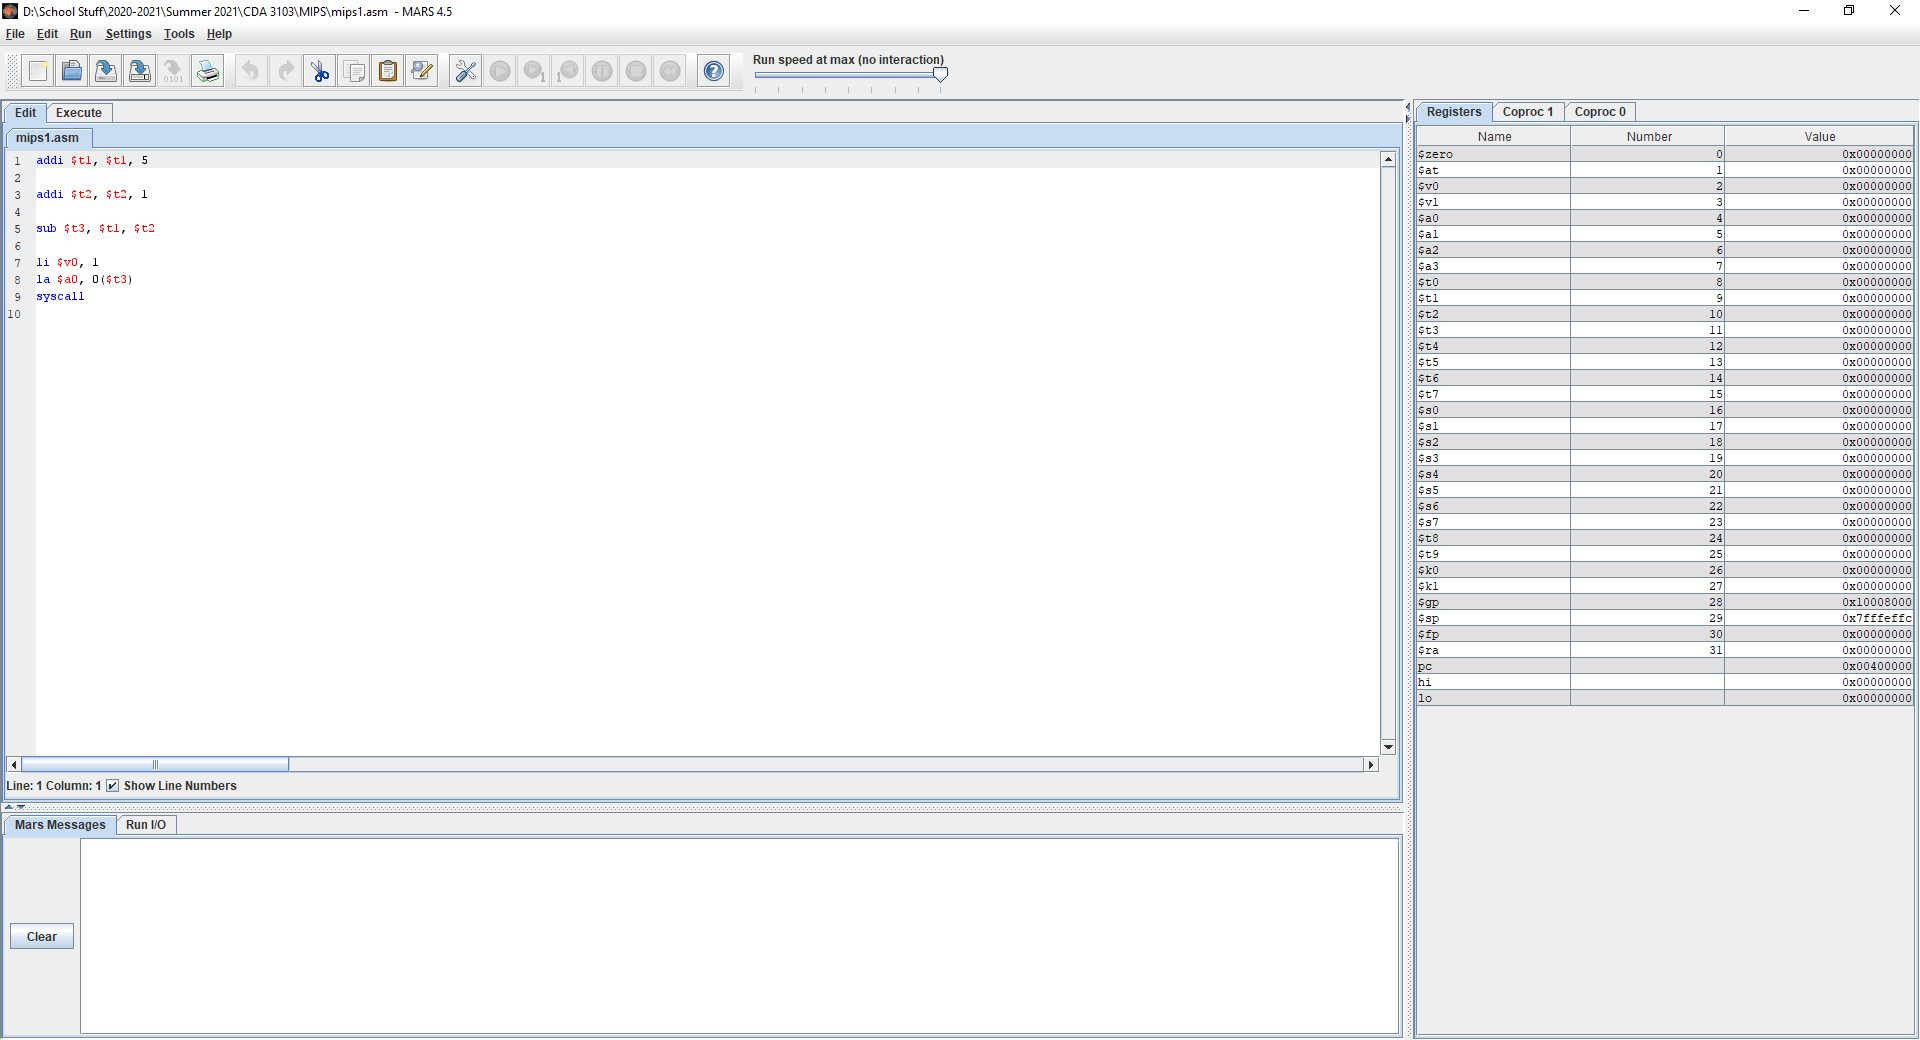
\includegraphics[width=\textwidth]{mars}
    \caption{Screenshot of MARS, a simulator for MIPS}
    \label{fig:mars}
\end{figure}

In addition to the windows, there are quick access buttons to easily
create, open, and save assembly code and more. These concepts of ``pick
up and code'' and ``call and response'' are keys to creating a simulator
that is engaging to the user and helps them understand these concepts.
While many of MARS's features and tools are nice, we do not want to over
engineer how it looks. We want the central focus to be how the code will
process through the datapath with graphs and animations. The current
methodology is to combine the registers window and some features from
the execute window to present a visual-rich representation of a MIPS64
Processor processing each line or provide the classic view like in
Figure \ref{fig:mars}. The ultimate challenge is fitting this all under
one browser tab, so it would be the matter of providing enough
information to the user on how the simulator works while providing a
free environment for them to do any MIPS project regardless of its
scale.

\subsubsection{Accessibility Features}
\label{subsec:accessibility-features}

For our website to truly be accessible to everyone, it needs to consider
how to get the most attention from users as well as being aesthetically
pleasing. In this section, we will discuss the choices we made to make
the site feel better to use for users of different accommodations.

\paragraph{Color Scheme}

Our color scheme choice must first consider the main color, the
secondary color, and the accent color. In Figure \ref{fig:mars}, for
example, MARS has a light-bluish color in some parts of its editor. We
will use the Monaco Editor API for our themes, custom or not.

The Monaco Editor API has the ability to define new themes, so if the
user is not comfortable with the default theme we have provided they
could also make a new one. First, let's look into how the theming for
Monaco Editor is structured:

\begin{itemize}
    \tightlist
    \item It starts with a base theme, which are the three built-in themes, vs,
          vs-dark, hc-black, and hc-light. They are self-explanatory, but if the
          user likes how one of them looks, they should be able to switch to it
          via a dropdown menu and start customizing from there. The three built in
          themes can be activated by accessing settings.js and editing the
          EditorTheme.
    \item There's the ``inherit'' parameter, which based on custom themes already
          provided \cite{monaco-themes} show that it is set to true to inherit the
          rules from the built-in themes, so that would be implicitly set by the
          program.
    \item The user would finally be able to set colors based on the tokens used in
          the MIPS language. While this could also be applied to other languages
          via Monaco, there are subtle differences to the type of tokens accepted
          by other languages; but in the context of assembly languages, they are
          fundamentally the same. It seems that the syntax for setting the color
          values is RGB-based \cite{rapidtables-rgb}, where the values are
          hexadecimal-based and the values assigned to the colors red, green, and
          blue are in pairs(i.e. \#FF0000 = red, \#00FF00 = green, and \#0000FF =
          blue). Some syntaxes for color values are 8-digit hex values, with the
          two last digits being the transparency of the color. The challenge will
          be to pair the tokens to the colors and create an interface that would
          let the user pick out a color and give it the appropriate RGB value, and
          to show the change in real-time would add more maturity to the
          application.
\end{itemize}

For this project we aim to have a light-bluish theme, since it fits with
the name SWIM. Tailwind CSS's color palette helps us in choosing the
right kind of blue for this project. We are currently planning for our
primary color to look like this (hex \#1D4ED8):

\begin{figure}[H]
    
\includegraphics[height=2cm]{color-primary}
    \caption{Primary color of SWIM.}
\end{figure}

As for our secondary color, we aim to have a lighter blue to simulate
swimming from the depth gradually up to the surface. This is the color
example (hex \#38BDF8):

\begin{figure}[H]
    
\includegraphics[height=2cm]{color-secondary}
    \caption{Secondary color of SWIM.}
\end{figure}

The accent is going to be gold in color, as it helps with complementing
the windows feel we envisioned for this app while also keeping our
uniqueness by making it fit the name SWIM.

\paragraph{Font Selection}

While the default Monaco font works well in terms of displaying code,
the user having the ability to select custom font size would improve the
readability of code for that user, as they can view it however they
like. However, Monaco Editor does not fully support styling or proper
sizing, but it has options for font weight, height, and family
\cite{monaco-fontsize-issue}. Another key feature that would help with
readability is the ability to toggle ligatures which Monaco Editor
supports. However ligatures are not actually necessary to be supported
in our Monaco Editor implementation, because we find that there is not
much use for ligatures for what we are trying to do. Not only will the
implementation be a little more difficult, ligatures are not used a lot
compared to the massively more used normal words, where other normal or
default Monaco fonts work fine.

\paragraph{Adjustable Windows}

Adjustable windows within the browser page is important for our app as
we cannot move the windows out of the browser itself and since some
users would have devices that use uncommon screen ratios which means
that implementing this is a necessity to have SWIM available across
multiple OS's and machines.

Spacing within our app, especially since SWIM is currently only
web-based, is vital to user experience. If there are too many windows,
or the windows are cluttered with details, the user may find it hard to
find what they need. This would also make the tutorial for first-time
users even harder due to having to point out many things. The tutorial
would also have a hard time pointing at what it needs to guide the user
on if windows are not spaced properly. For those reasons, users being
able to adjust how wide they want the sections within the app to be is
beneficial to accessibility.

Users can also have custom screen resolution and ratios, especially
through different devices and operating systems of their computers, This
is where dynamic screen size support comes in. The web app will
automatically adjust the original ratios of the windows in the program
so that it matches the ratio of the monitor, or whatever the user set
their system's resolution to be in. As of currently when this topic is
discussed, there may be a problem with implementing this as it will have
to be tested within a variety of window sizes within browsers. The first
step to achieving this is for the app to be able to resize and ratio
itself when the browser minimizes or changes size, which should be able
to come along with the browser's app handling.

\subsection{Loading and Saving}

How loading and saving files work in SWIM is that it will be able to
load assembly files (.asm) and text files (.txt), as well as MIPS files
(.mips). In this section, we will focus mostly on the text files, how
they work and how SWIM handles loading and saving those. The main
advantage of loading and saving files is that the workflow for the user
will be more intuitive, no need to copy and paste your code onto a text
editor just to put your code onto SWIM for loading. However due to the
limitation discussed in \ref{subsec:pack-bindgen}, we implemented the
ability for the user to copy their code onto their clipboard so they can
paste it in a text editor like Notepad. The reason we can load and save
these files is due to how Monaco Editor only loads in strings. However
due to Rust's persistence on using UTF-8 encoded text, some invalid data
cases (i.e. transforming a .exe to a .txt with UTF-8 encoding) will not
compile and crash SWIM. We should take note of this if we want to safely
load a file by having the application only accept certain file types via
the \texttt{accept} attribute from a \texttt{file \textless
    input\textgreater{} element}, which will be explained later in this
section. However, if a user has a text file that lacks any MIPS syntax
then the parser will be able to notify the user that the file will not
compile but should allow the user to ``work'' on it as if SWIM is a
regular text editor like Notepad. When SWIM starts up, it will provide a
template file for the user to store their variables and strings, and how
to structure their code(main block, labels, etc.). The template file can
also be an empty text file or formatted file for the user to be able to
structure code if they do not have anything else to work with.

The File API \cite{mdn-file-api} allows the web applications to access
files and their contents. The user can let the application access them
by using a file \textless input\textgreater{} element or ``drag and
drop''. The former would prompt the user to select a file from their
computer and the UI will based on which operating system is currently
running, but the latter will allow the user to drag their file onto SWIM
and load it from there. ``Drag and drop'' is more involved using the
\texttt{files} property of DataTransfer (\texttt{DataTransfer.files}),
but it is safe since this property can only be accessed from within the
\texttt{drop} event and all the other events will have the files
property emptied. This does introduce a problem if the user wants to
drop multiple files onto SWIM, but this could be remedied by only
opening the first file in that list. For the philosophy behind only
being able to load in one file at any given time, read Section
\ref{subsec:lack-of-project-tabs}.

While loading files is simple, it is the process of saving a file that
is a bit more tricky. While Chromium and Edge utilize the File System
Access API to make the process simple, Firefox does not support this
API. Most browsers support IndexedDB, however with the current
development ecosystem for SWIM, we think it is excessive since we only
want to save source code and graphs of the datapath. Firefox can use a
subset of the File System Access API called File and Directory Entries
API which should cover the browsers that support WebAssembly. The File
System Access API lets us read files, load and save files, and give
access to directory structures. The interaction with files and
directories are done through handles with the parent class,
\texttt{FileSystemHandle}, helps define two child classes:
\texttt{FileSystemFileHandle} and \texttt{FileSystemDirectoryHandle}
respectively for file and directory handling within a user's system.
From there, we could utilize methods to call the user's file or
directory picker via \texttt{window.showOpenFilePicker} and
\texttt{window.showDirectoryPicker}. When they are called, a window will
open that would allow the user to select a file or directory and once it
is selected then a handle is returned. Another method to access file
handles is through \texttt{DataTransferItem.getAsFileSystemHandle()}
method of HTML Drag and Drop API. This API has ``save'' functionality
using the \texttt{FileSystemWritableFileStream} interface, which will
save the data stream as a Blob, String object, string literal, or
buffer. This can be done on a new or existing file. The subset API, File
and Directory Entries API \cite{mdn-file-and-directory-entries-api},
functions similar to File System Access but it simulates a local file
system that a web app can navigate within and access files in. Within
the virtual sandboxed file system, the web app can read, write, and
create files and/or directories. There is one last method that could be
utilized to save files, and it is through the Web Storage API which is
the alternative for saving session data. This means that we do not have
to worry about any compatibility issues, so no need to over engineer a
system to save files.

All of this is under the assumption that we could treat SWIM's saving
system as if it is a desktop application, but another paradigm to this
system is if we treat it as if you are downloading a file rather than
constantly writing new data to the same file. Of course this would lead
to multiple versions of the same file being saved, but it should not be
an issue due to the size of the source files. The location of the files
will be based on where the user set their browser to download the files
onto, and the filename of the download files is ``SWIM'' plus the
current time the file was saved to make it distinctive to the user. The
caveat with this system is that Apple Safari does not have direct
support for the Downloads API, however it does have its own method of
fetching files from the web \cite{apple-downloading}. How it works is
that we have to create a \texttt{URLSessionDownloadTask} from a
\texttt{URLSession}. The documentation from Apple recommends for simple
downloads, downloads that lack progress updates, to use a completion
handler. This will be called when the download ends, either as a
successful or a failed process. It may receive a client-side error,
indicating a local problem (i.e. unable to connect to the network). If
there is none, then we will receive a \texttt{URLResponse}, which should
be inspected to ensure it indicates a successful response from the
server. If the download was successful, then the completion handler
receives a URL indicating the location of the downloaded file on the
local filesystem. This storage is temporary, so to preserve the file it
must be copied or moved from the location before returning the
completion handler.

While these APIs are great, we lack some form of a database and FTP
system to properly implement this so we resorted to an alternative of
copying the code onto the clipboard. Once that is done, we tell the user
that the code has been copied and it can pasted onto a text editor with
the paste shortcut provided to them to save locally.

It is entertaining to see how ubiquitous the web browsers are when it
comes to loading files, but saving files is a challenge in itself. The
best way to tackle saving is to create a catch-all function that would
filter out the correct API for the specific browser that is in use, but
it would be wise to tackle Chrome and Firefox first due to the multiple
devices supporting them and the fact that they both support the
Downloads API. Now the debacle over the methodology of saving files is
due to the controversial topic of user's giving browsers access to their
device's functionalities. Safari denied support for APIs like Web
Bluetooth, Web NFC API, User Idle Detection, and more since they would
make digital tracking easier for advertisers \cite{cimpanu2020}.

\subsubsection{Code Execution}

One of the core functionalities with SWIM's front end is executing the
actual code, otherwise it is about as useful as a text editor that looks
like it can run MIPS. The only information we have to pass to get the
execution going is the text the user inputs into the Monaco Editor
window and it follows the appropriate syntax. The main challenge of this
is that we have to pass in the necessary information to the parser which
would pass it to the emulation core and present it in a way that the
user knows that it is executing in front of them while only having the
space of a single window.

We have two modes of execution, step and stage, which would be activated
with a press of a button at the top of the window. Normal execution is
where the code gets sent to the parser to transform it into bytecode,
which gets sent to the emulation core to process it. The core would
process every line until there is no more code or there's a line that
causes the system to stop, either from a crash or syscall. This means
that the user will only see the last processed state of the emulation
core via the console and register windows, however this was not
implemented due to the lack of an interrupt system for SWIM. Step
execution is much more interesting from an educational perspective. The
user will get to see how each line is processed, and the previously
executed line would be highlighted to make the flow control more
explicit and hopefully make debugging logic errors easier to find. The
highlight would be designed to contrast with the default theme
appropriately. MARS has speed control with executing code measured by
instructions per second, but we rarely saw any use for it since it is
like the normal execution mode but slow. A brand-new form of execution
is excuting by stage, which is similar to step execution but it will
execute the stage within the single-cycle datapath. The lines that
correlate to the stage that was previously executed are highlighted on
the datapath. The nice part about the design of the step execution mode
is that everything is visually communicated to the user, there is no
need for the console to show any information unless it pertains to user
I/O. With addition to step-execution, we could apply the rewind function
through this to improve the debugging process. It is important to note
that we give users the ability to reset the datapath at any point during
execution as a panic mechanism, i.e. an infinite loop.

\begin{figure}[H]
    
\includegraphics[width=6cm]{mars-execution-buttons}
    \caption{The execution buttons shown in MARS: Execute, Step-execute, Rewind, Pause, Stop, and Reset.}
\end{figure}

\subsection{The Register Window}

The register window will show two tabs to show two different types of
registers: general purpose (GP) and floating-point (FP). General purpose
registers are used primarily to supply data for most instructions, as
well as to move data to floating-point registers. Floating-point
registers are used for instructions involving the floating-point unit.
Registers are transferred to the front end by the API provided by the
emulation core. Details on the MIPS specification of general purpose and
floating-point registers are described in Section
\ref{subsec:mips64-registers}.

The register window shows the values of registers in decimal by default,
but they can be converted to hexadecimal or binary with a press of a
button, additionally making SWIM more unique than other emulators with
register viewing functions. This converting functionality will help
understanding values in registers better, as users may have a preference
between reading binary, decimal, or hexadecimal formats.

\subsection{The Help Button}

The Help button is important for anyone who uses any website, as it is
where the user usually gets answers on how the website works in general
or what the smaller, more obscure button on the screen does in the
website. SWIM is the same regarding that. It is planned that the help
button will be placed on the top right of the website, above the
register window. Pressing the button will have a pop-up on the screen
with the questions and answers for some of the most important details to
know in order to use MIPS. The help pop-up can also appear during a
user's first time usage of the webapp.

The details needed for the tutorial inside the Help command is of a lot
of importance. For a simulator of MIPS, it may be clear that aside from
people with previous coding experience, new users may not even know what
to start or do with the website. As such, the first thing the help
section will have is how to type up instructions for MIPS, as
instructions are an integral part to the MIPS learning experience. It
will show some examples on the instructions to type up. The Help section
will then show the different types of instructions that can be made in
the website, or in other words, instructions that this website will
support running. Details on what instructions will be supported can be
found in Section \ref{subsec:supported-instructions}. With how many
instructions there are, we also want to implement a searching
functionality within the help pop-up to search for specific answers for
the users' questions. Some questions will have the answer pointing the
user towards User Settings, which is located

However, with that having been said, we are also debating if the help
section is worth making. For the reasons stated in the beginning, we do
agree to implement it, but it may be difficult for the amount of things
it does.

\subsection{The Lack of Project Tabs and Why}
\label{subsec:lack-of-project-tabs}

Having a development environment capable of loading in different
projects seems like it is a given, however we agreed that a feature like
that is not needed for SWIM at its current state. Historically, assembly
programs followed the same philosophy as modern programming with
breaking up large functions into smaller code that would interact with
each other to achieve a certain task. A great example is that most
vintage arcade systems rely on a dual CPU setup, one to drive graphics
and game logic and another to drive the sound system itself.
Additionally, these two CPUs would have different architecture, i.e.
Motorola 68000 and Zilog Z80, so programmers would have to figure out
ways for the two CPUs to communicate. However with MIPS Assembly for
college students, they are only learning how code is processed at the
lowest human-readable level. Most of the projects in-class consists of
learning flow control, how floating-point numbers are calculated and
stored, and concludes with implementing the bubble sort. Fundamentally,
most of those assignments might require a lot of lines but do not need
to be broken up to separate source files. Also, the mileage of SWIM
relies on all parts, so if one part of SWIM is not up to standards then
it really limits the student on what they can learn about MIPS as a
whole.

\begin{figure}[H]
    
\includegraphics[width=\textwidth]{vscode-tabs}
    \caption{Multiple tabs being opened in Visual Studio Code, note the different languages being loaded in.}
\end{figure}

Here is a list of why multiple project loading is not being considered,
from the front-end down to the core itself:

\begin{enumerate}
    \tightlist
    \item
          {[}Front-end{]} Having multiple project tabs open would lead to
          navigating between them harder. Learning how web browsers handle
          multiple tabs, it seems like grouping tabs is a great solution for
          organizing them but it would lead to some overhead with how the Monaco
          window will have to keep track of the multiple instances in terms of
          giving the correct one to the parser. The memory and register
          windows should only change based on which file is currently being
          executed, and if a user wants to execute another file while one is
          still running then we should provide a panic button which will
          reset the datapath.
    \item
          {[}Parser{]} One of the key features that we want the parser to do is
          to communicate with the user in assemble-time about most errors to save
          time on debugging their code. However, it will be extremely difficult
          to have it functional if the Monaco window has to juggle between
          multiple instances to send them to the parser. With the current design of
          the parser, it would be wise not to constantly send updated text to it
          as it would penalize our performance.
    \item
          {[}Emulation Core{]} Despite how well-designed a core might be, it is
          only good at focusing on what is currently being done. Having multiple
          projects would only get in the way of constructing an user-friendly
          environment for someone who is new to the concept of assembly
          programming. What if a user wants multiple projects running on
          different datapaths? Then, it would require us to have multiple
          instances of the core at different settings which would lead to lower
          performance.
\end{enumerate}

Overall, having the ability to load multiple projects is a simple
``nice-to-have'' but it undermines the fundamental goal of what we want
SWIM to be. As we incorporate the visual datapath and further develop it
into a mature MIPS emulator, we will disregard the notion even more and
focus on implementing features that would make SWIM fun and rich to use.
Besides, loading and saving a different project is as easy as pushing a
button. The only valid case for implementing multiple project tabs is if
we redesign the entire interface to allow different emulation cores and
parsers to interface since everything is being designed with MIPS in
mind currently.

\subsection{Displaying Errors}

With SWIM's parser handling recognizing errors and categorizing them in
an explicit fashion, it is up to the interface to take what the parser
has interpreted and show it to the user. The fundamental challenge is
how to display it. The system in place to allow this is to have the
parser create an API call to get these messages and organize them on
what type, then display them in an appropriate fashion.

The first method is to display the error messages within the console
window. In order to make the error messages distinct from the rest, we
will employ a structure that should be easy for the user to understand
as followed:

\begin{center}
    \textless Line \#\textgreater{} : \textless{[}error type{]}\textgreater,
    \textless error message\textgreater, \textless possible
    solution\textgreater{}
\end{center}

Since MIPS is assembled by line, it should be simple enough for the
error to be located and to properly communicate its type and how to fix
it. This should be sufficient enough for the user to differentiate the
messages shown on the terminal, and should alleviate the problem of
having a separate tab within the terminal only for error messages. In
order for any program to show any prompt for user I/O, the program has
to be assembled properly in the first place so there should be no
overlap between the two. The errors will display when the user is
attempting to assemble their erroneous code.

The second method is to hover over incorrect lines to display the
message that way, however the challenge would be differentiating those
messages from hovering over to another area that could show the user
what the instruction does. Fortunately with the MIPS syntax
highlighting, we could take advantage of how it parses through code.
When it casts a red underline for certain lines, we could have the
cursor hover over the specific line number or general area to show the
message that way.

\subsection{Interactive Graphical View of Datapath}
\label{subsec:datapath-visual-representation}

% NOTE: This section used to have a reference after "WepSIM" to the section
% that discusses alternative MIPS emulators.

One of the key stretch goals of SWIM is the ability to view a live,
interactive version of the simulated MIPS64 datapath. This functionality
is largely unique to this project and does not exist in many other
alternative MIPS emulators, with the exception of WepSIM. It has been
shown through a number of studies \cite{presmeg2006, carney2002} the
benefit of using images and graphics to study concepts, thus for the
educational purposes of SWIM, offering an interactive, graphical view of
the datapath is essential for understanding computer architecture
concepts at a deeper level.

Despite there not being many animated visualizations for datapaths,
there are many close alternatives in other areas that can be used as
context for the style and view of the variation of this feature as it
exists in SWIM. For instance, many video games that focus on low-level
circuitry mechanics (such as Minecraft, NandGame, and Turing Complete)
allow players to expose individual pieces of wiring interactively to
gain a rich understanding of the data and signals that pass through
these systems \cite{minecraft, nandgame, turing-complete}. Figure
\ref{fig:turing-complete} offers one such example of this concept.

\begin{figure}[H]
    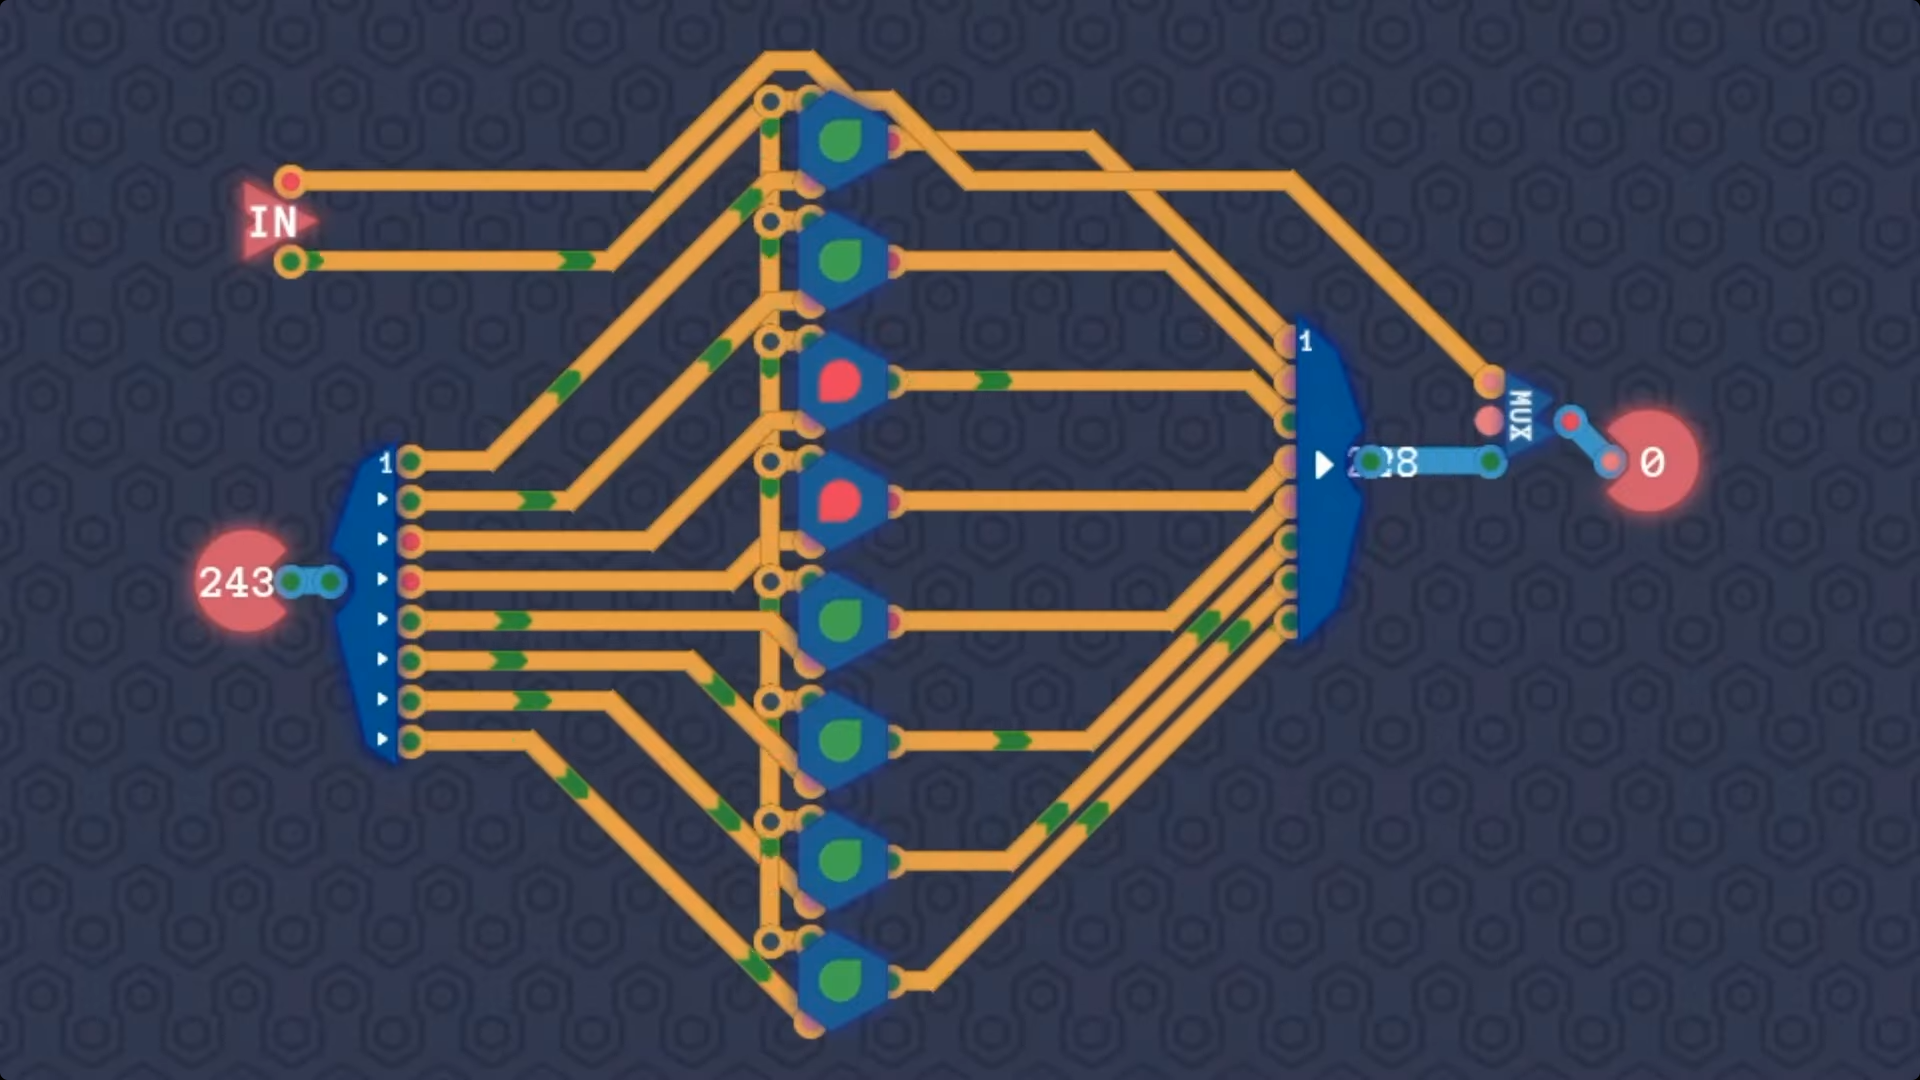
\includegraphics[height=7cm]{turing-complete}
    \caption{Example of viewing individual bits in a system. Screenshot from Turing Complete trailer \protect\cite{turing-complete-trailer}.}
    \label{fig:turing-complete}
\end{figure}

While these offer compelling use-cases in their own regard, this
highly-granular view to circuitry can be overwhelming or unnecessary
when studying in the scope of computer architecture. As an example,
individual AND and OR gates are typically abstracted from view when
viewing more complex components of a datapath, such as register files or
memory.

Another common view of circuitry is by a static image. While not
interactive or animated like the aforementioned approach, this format
tends to have a more appropriate level of abstraction, and is commonly
seen in computer architecture textbooks and course lecture slides. This
form of visualization has become the de facto standard despite these
limitations.

With this context, it can be seen the importance of a both interactive
and properly-abstracted graphical depiction of a processor. The primary
way to view the active portions of the datapath is by highlighting the
wires of the datapath associated with the current stage. This is a
simple yet naive approach to this, as there is no differentiation
between wires that are active versus inactive. Despite this limitation,
this is planned to be the first iteration of this visualization feature.

\begin{figure}[H]
    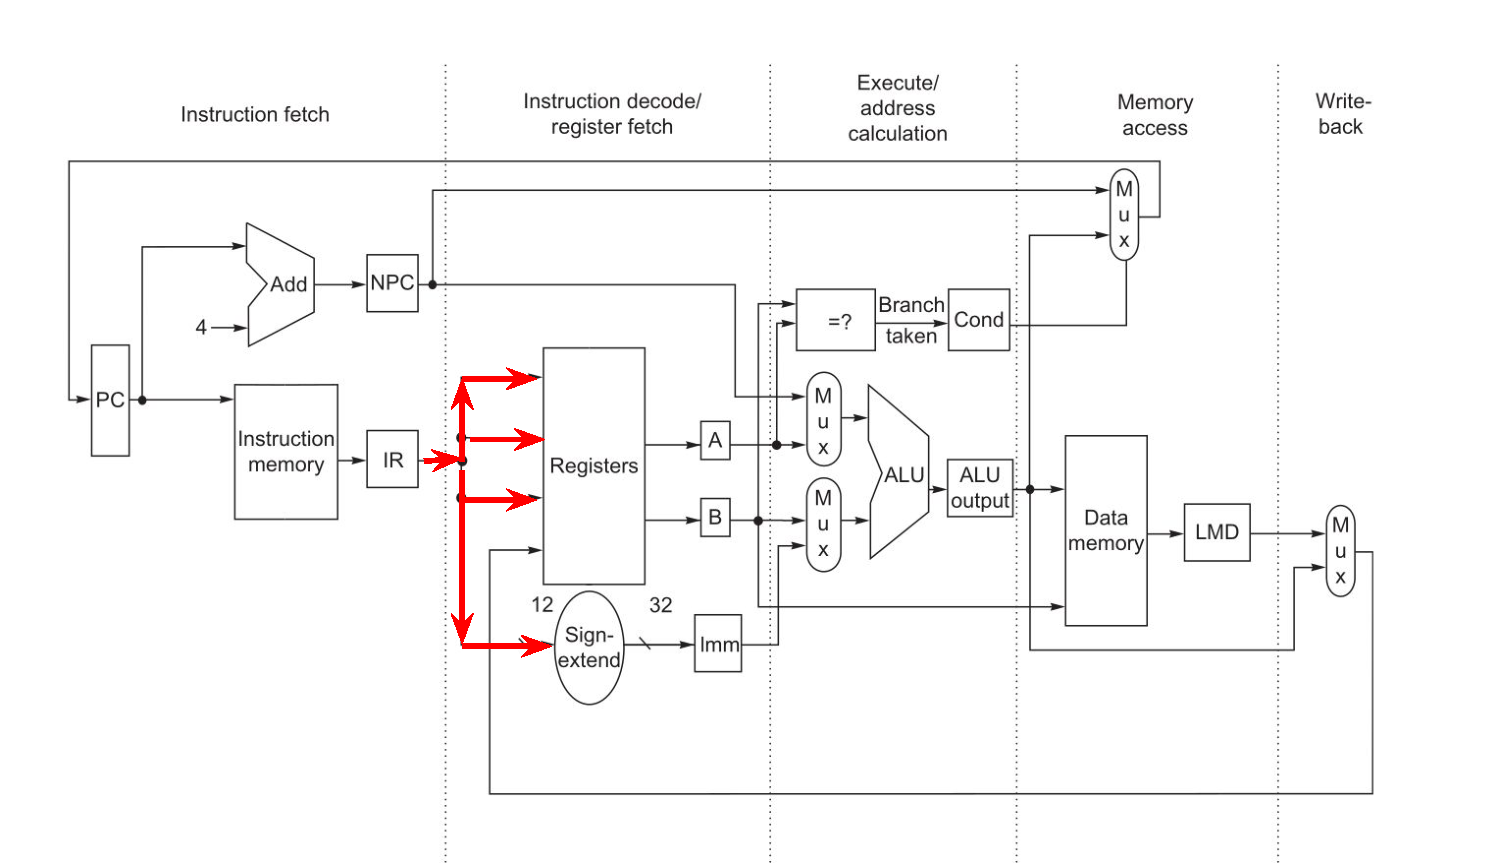
\includegraphics[width=\textwidth]{mips-graphical-view-staging}
    \caption{Example of the first planned iteration of the interactive graphical view feature. Original image from \protect\cite[p.~287]{hennessy-patterson}.}
\end{figure}

Future iterations of this highlighting functionality would allow for
specific lines to only be activated when they are selected by a
multiplexor, for example.

An additional aspect of this interactive graphical representation is the
ability to hover over specific lines and elements in the datapath to
view their contents. These contents would include a name of the selected
elements, its description, and the current value associated with that
element. The user would also be able to view the meaning of the value of
the element, as well as other possible values of that element. In the
case of data lines, there would be no description to the value, but
instead a raw binary representation with a decimal or floating-point
representation, depending on the specific line. Figure
\ref{fig:hover-over-mockup} illustrates the case of viewing a data line.

\begin{figure}[H]
    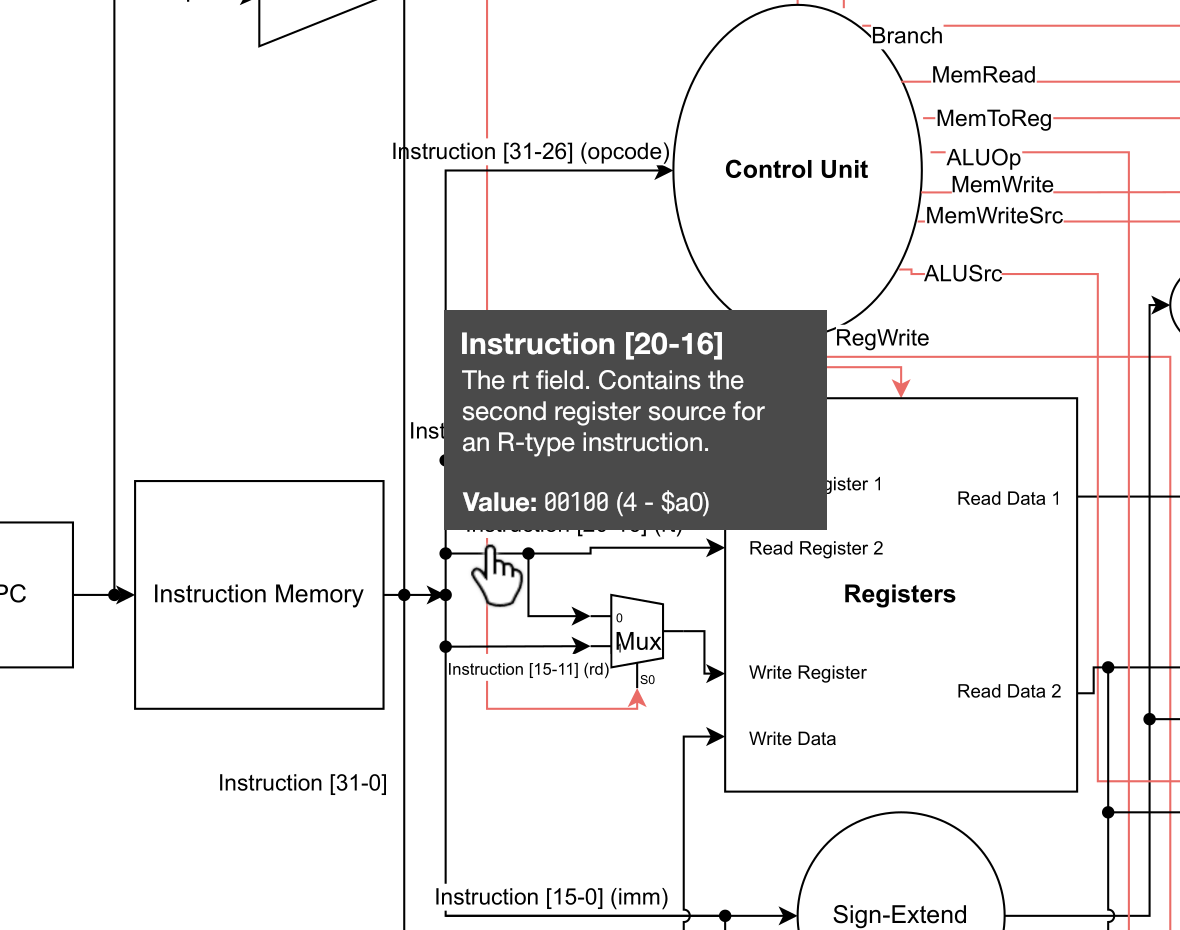
\includegraphics[height=8cm]{hover-over-mockup}
    \caption{Example mock-up of hover-over line description.}
    \label{fig:hover-over-mockup}
\end{figure}

To implement this feature, a number of design aspects must be considered
in both the initial drawing of the datapath and the rendering of the
datapath. An important consideration when selecting software to sketch
the datapath is the ability to tag and label elements by stage and by
element. After cursory research, it was decided that the datapath would
be sketched from scratch using Diagrams.net for its ease-of-use and
access. In addition, Diagrams.net has the ability to add tags and
additional metadata to each element. However, by default this metadata
is not exported in any format other than the format specific to
Diagrams.net, .drawio. With no standardized method of importing and
reading this export format, this would not be feasible to use. Despite
this, Diagrams.net offers an SVG add-on that adds support for including
metadata in SVG file exports. As the vector graphics format is
widely-supported by third-party tools and libraries, this was decided as
the methodology for exporting the raw datapath.

With an exported SVG file containing the simulated datapath, the second
consideration is the method of importing this file into a renderable
format in a web browser. Initially, a \textless canvas\textgreater{}
element was considered for rendering, as its flexibility and ability to
use vector graphics were ideal. However, there were issues surrounding
the rendering of the datapath, as the datapath is highly complex and
must be zoomed to avoid loss of detail or an improper resolution.
Instead, direct vector graphics were decided as a necessary alternative.
This methodology allows individual lines or groups of elements to be
controlled directly using Javascript or Rust code.

An alternative version of this feature, not within the scope of SWIM's
stretch goals, is to instead highlight and show lines in a datapath
modeled against a real-world die image. Due to its high complexity, this
was not considered for implementation, but is a possible alternative for
other datapaths or processor architectures. This feature largely mirrors
the visualization as described by \cite{wojtowicz2015}.

\begin{figure}[H]
    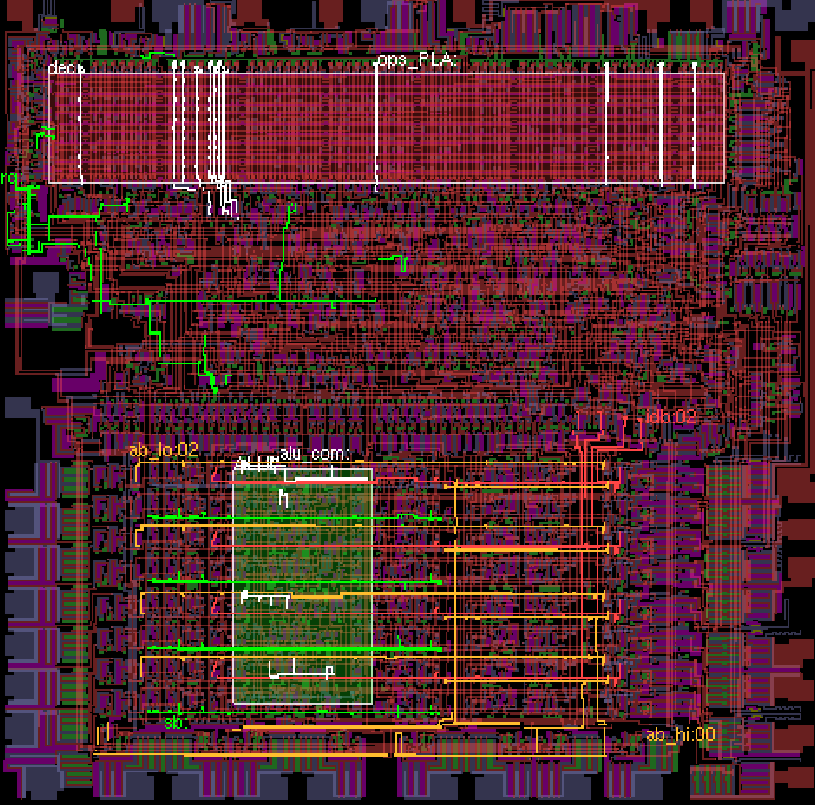
\includegraphics[height=10cm]{wojtowicz-visualization}
    \caption{Proposed visualization approach with internal buses and datapaths shown, combined with overlay for selected functional components. Sourced by \protect\cite[Fig.~2]{wojtowicz2015}.}
\end{figure}

This interactive view, while designed to work specifically with the MIPS
architecture, can be expanded easily to work with other platforms and
architectures. Extensibility will not be a major aspect of design for
this feature, but there will be some consideration to at least keep it
modular and separated from other components of the codebase.

\subsection{CSS}

One of the fundamentals when it comes to developing a web application is
Cascading Style Sheets (CSS). It is used for styling and laying out all
the components onto the browser. With the discussion about SWIM's
accessibility features (Section \ref{subsec:accessibility-features}),
CSS is required to realize those features. Yew, unfortunately, does not
have integrated CSS support however we can utilize component libraries
to make the design implementation easy for the team and nice to look at
for the user. While there are many options, we want to use libraries
that will not have a strong reliance on JavaScript in order for the
codebase to be consistent and readable in the future. Here are the
candidates for SWIM:

\begin{enumerate}
    \item
          \textbf{stylist-rs} -- This is the most active repository for
          implementing CSS into Rust, and there are multiple ways to implement
          the CSS which makes it really flexible. To keep it brief, we are
          only going to go into the \texttt{macros} and \texttt{yew} modules
          in the crate since the \texttt{ast} and \texttt{manager} modules are
          not stable or too advanced for the project.

          The macros module \cite{stylist-macros} is what makes CSS possible in
          Rust, \texttt{css!} is similar to the \texttt{format!} macro which we
          could write in the styling rules as a string literal followed by an
          argument list. The macro will replace \texttt{\$\{arg\}} with the
          argument in the argument list when creating the AST. If we do need to
          print a ``\$\{'' sequence, then we may use ``\$\$\{'' to escape to a
          ``\$\{''.

          \begin{figure}[H]
              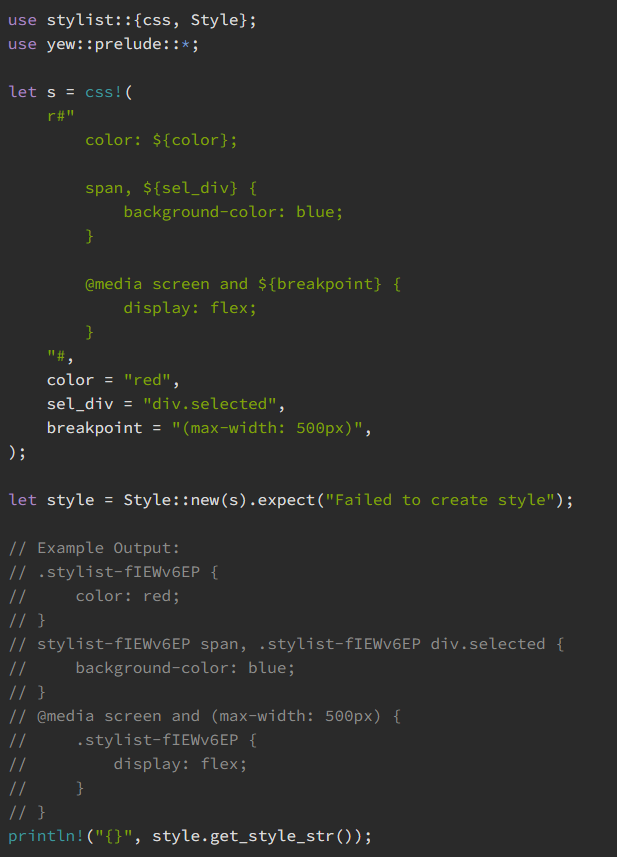
\includegraphics[height=14cm]{stylist-rust-example}
              \caption{Example code of how CSS is done in Rust with stylist. Note how the arguments are handled with ``\$\{\}'' to easily store and edit definistions and all of it is encapsulated within the ``css!'' macro. This will output the appropriate CSS below it.}
          \end{figure}

          There are limitations to the format due to rustc's tokenizer. For
          example, ``4em'' would be tokenized as a floating point literal with a
          missing exponent and a suffix of ``m''. To workaround this, we could use
          interpolation as in \texttt{\$\{``4em''\}} and this could be applied to
          some color hash-tokens like ``\#44444e'' to \texttt{\$\{``\#44444e''\}}.
          There are more intricacies with the tokenizer and how it interprets CSS
          syntax, but Rust is still trying to sort these edge cases of parsing out
          so workarounds had to be implemented.

          The yew module lets us insert CSS directly onto functional components
          via ``styled components'', this time it uses the \texttt{use\_style!}
          macro to parse literal strings or an inline stylesheet to be used within
          \texttt{html!} macros to create auto updating styles.

          \begin{figure}[H]
              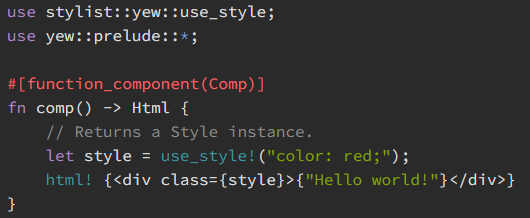
\includegraphics[width=0.75\textwidth]{stylist-rust-component}
              \caption{An example of a styled component. Note that it uses a different macro ``use\_style!'' and looks similar to an internal stylesheet, having CSS inside a HTML document.}
          \end{figure}

          From a glance, this library may look like a challenge since it is CSS in
          Rust but it has a good underlying point going with JavaScript not being
          used to achieve the implementation. However, it seems like this is meant
          for developers who are comfortable with Rust and front end development.
          It is important to note that there are multiple ways to achieve CSS in a
          Rust web application, and this one is meant to be a stepping stone to
          implement this onto Yew.

    \item
          \textbf{styled-yew} -- This was an early attempt with implementing CSS
          into Rust. The way how you write it in is:

          \begin{verbatim}
styled!(pub RedDiv : Div {
    color: "red";
});
    \end{verbatim}

          With \texttt{styled!} being the macro to write in CSS rules for the
          application and the component being visible for the code to use with the
          familiar structure we have to give a certain area of the page color,
          font-weight, etc. You can then use them inside the \texttt{html!} macros
          like we would inside a html file. This has not been worked on in over
          two years and lacks documentation and real-world examples.

    \item
          \textbf{yew\_styles} -- This is a styling framework that does not
          require any JavaScript dependencies and creates a layout system that
          is closely related to the flexbox concept. It also takes Rust's
          benefits and implements properties selected by enumeration, which
          makes the process of developing applications efficient. The framework
          splits the components into two parts, the yew component and its sass
          module, although the sass module only needs to be included into the
          project. While this framework was enticing with trying to lower
          dependency for JavaScript, the documentation is really poor and the
          examples that use this framework are not available and the last commit
          was made in November 2021.

    \item
          \textbf{muicss-yew} -- This is a component library for Yew framework
          based on the lightweight MUI CSS framework. MUI follows Google's
          Material Design guidelines and was designed to be fast, small, and
          developer friendly. It has a small payload size, no external
          dependencies, and more. While the library and MUI JS are still in
          development, the supported components are enough to create SWIM as
          shown with the Figma prototype. If the component that is needed is not
          in the muicss-yew, then we have to use MUI-CSS directly with Yew which
          might result in losing readability since we introduce JS and CSS onto
          the file system. This will give us an ultimatum in terms of how the
          project is structured in the future, do we use the library as-is and
          wait or implement bindings to components we need or use MUI with JS
          and CSS to get all of the features from the beginning. The library has
          not been worked on since April 2021, so to be safe in terms of SWIM's
          longevity we will not use it.

    \item
          \textbf{Tailwind CSS} -- Tailwind is a popular framework to be used
          and is being praised for its workflow, code structure, and
          customization options. It is favorable enough to have three methods
          to implement it into a Yew project. The first one
          \cite{dev-to-tailwind-css} is to require JavaScript to build
          Tailwind CLI which would output a .css file for us, then we insert it
          into the index.html file. From there, we insert the appropriate CSS
          classes within the \texttt{html!} macro then \texttt{trunk serve} for
          deployment. The initial output file will be large, but can be
          trimmed down with a config.js file down to the classes that were
          used. The alternative \cite{tailwind-yew-builder} to this does not
          use JavaScript (npm) and instead Docker to build Tailwind CSS, but
          the build process is the same with \texttt{trunk serve}. The last one
          \cite{tailwindcss-yew-template} is a starter template which requires
          Tailwind and \texttt{tools} installed with npm used to run and install
          the app, while the workflow has not been worked on for some time it
          is an option. With Tailwind's documentation and how the
          implementation of the first two methods has us write CSS in a
          readable format, this is a viable option to use as SWIM's CSS
          framework.

    \item
          \textbf{ybc} --  A Yew component library that is based on the Bulma CSS
          framework. This one does not aim to encapsulate Bulma types to Rust
          types since it would be too complex and limiting for the developer.
          The format to implement the styles is much nicer and in-line to what
          you would see inside most CSS files, and linking to the .css file to a
          .html file is simple likewise with sass files for customization
          support. It has Trunk support for developing and the codebase is
          structured in a way that you can easily correlate the categories to
          Bulma's documentation.

          \begin{figure}[H]
              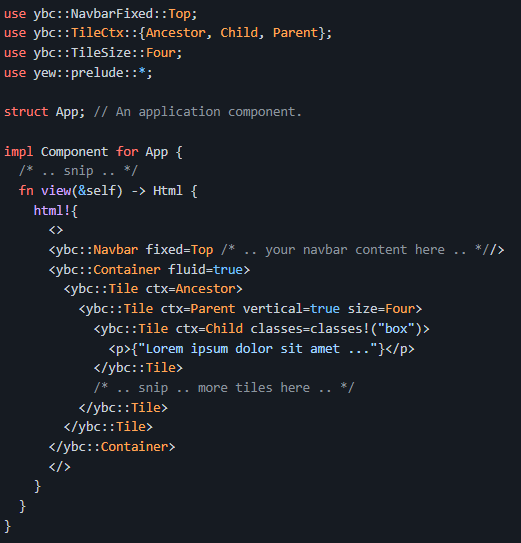
\includegraphics[height=11cm]{ybc-example}
              \caption{Sample implementation of ybc in Yew within a component's view method using a navbar, fluid container, and tiles.}
          \end{figure}

    \item
          \textbf{patternfly-yew} -- To keep it brief, this is similar to the ybc
          in terms of how the codebase is structured and comes with a sample
          project to see how Patternfly works in a Yew project. A lot of effort
          went into binding the components, but it shows off what Patternfly can
          do and rather well. A strong candidate for a CSS framework.

    \item
          \textbf{yew-feather} -- A Yew component library that lets us use
          Feather v4.28.0 for icons, this was succeeded by yew\_icons. One of
          the advantages that Feather has is that we can assign a color value to
          the icons, so it can be added as a customization option to make SWIM
          look nicer.

    \item
          \textbf{yew\_icons} -- Same as the one above, but is more active and
          contains even more collections of SVG icons like Feather, Bootstrap,
          Octicons, and more. There is an interface for using Octicons in Yew
          with examples, so there is promise with Icon support for Yew. The main
          thing to be aware of when it comes to importing the icons needed for
          the project is to explicitly state them within the dependencies field
          in our project's .toml file.
\end{enumerate}

With all of the probable options laid out, it is imperative that we
follow the responsive web design (RWD) protocol given that it is having
different components interacting (register window, console/memory/visual
datapath window, monaco window, and buttons). It is a ``design approach
that addresses the range of devices and device sizes, enabling automatic
adaptation to the screen, whether the content is viewed on a tablet,
phone, television, or watch'' \cite{mdn-responsive-design}. The relevant
methods of implementation would be for the user to be able to adjust
sizes of the windows at will (i.e. dragging the border between the
Monaco and console/memory/visual datapath window to get more room for
either window, or scaling the text based on the size of the main window.
There are multiple situations that will arise that will force us to
think this way in order for SWIM to look professional across all
platforms. The Monaco Editor is a challenge with this since it has its
own CSS system, so we have to be mindful of making the two look
cohesive. For SWIM, we used raw CSS to style the page and codicon, the
icon library for Monaco Editor, and font awesome as our icon libraries
to make SWIM look modern as Visual Studio Code.

\section{Project Management}

\subsection{Project Milestones}
% TODO: Update milestones?

{\renewcommand{\arraystretch}{1.4}
    \begin{tabularx}{\textwidth}{|l|X|}
        \hline
        \textbf{Date} & \textbf{Milestone}                                                                                                                                                                                                                                                                                                                                                                                                                   \\\hline
        9/19          & Group introductions - Initial date to meet team members, discuss goals and ideas, and to schedule weekly meetings.                                                                                                                                                                                                                                                                                                                   \\\hline
        9/23          & First regularly-scheduled group meeting - Collaboration on project requirements, choice of language(s) and framework(s), and project roles. \newline \textbf{Note: Every future regularly-scheduled meeting may not be listed here.} \newline \newline Group members begin self-learning the language and frameworks planned to be used for this project (Docker, Rust, Yew). Collaboration on the initial design proposal begins.   \\\hline
        9/27-10/4     & Get taken out for a week due to Hurricane Ian. :')                                                                                                                                                                                                                                                                                                                                                                                   \\\hline
        10/5          & TA check-in \#1. (Show 3-5 pages contributed per member)                                                                                                                                                                                                                                                                                                                                                                             \\\hline
        10/7          & Regularly-scheduled group meeting - Final discussion, clarifications, and wrap-up of the Initial Design Proposal.                                                                                                                                                                                                                                                                                                                    \\\hline
        10/7          & Assignment 3 (Initial Design Proposal) is due. (15 pages total)                                                                                                                                                                                                                                                                                                                                                                      \\\hline
        10/10-10/14   & Discuss project architecture scale and determine required features and stretch goals.                                                                                                                                                                                                                                                                                                                                                \\\hline
        10/10-10/14   & Research and set up the version control system to be used for the project.                                                                                                                                                                                                                                                                                                                                                           \\\hline
        10/17         & Begin discussing interface design between front-end team members.                                                                                                                                                                                                                                                                                                                                                                    \\\hline
        10/17-10/21   & Research and set up the system to be used for linting code, running tests, and using these with a continuous integration system.                                                                                                                                                                                                                                                                                                     \\\hline
        10/19         & Meet with Dr. Gerber to check progress and understanding of the project.                                                                                                                                                                                                                                                                                                                                                             \\\hline
        10/21         & Regularly-scheduled group meeting - Project status and design document review.                                                                                                                                                                                                                                                                                                                                                       \\\hline
        10/24         & Begin discussing the emulation core structure and supported internal API calls. These API calls are used for the web interface to communicate with the emulation core.                                                                                                                                                                                                                                                               \\\hline
        10/24-10/28   & Research and set up the hosting, server, and deployment solution for the project.                                                                                                                                                                                                                                                                                                                                                    \\\hline
        10/31-11/11   & Each member creates a basic small project of their own, resembling the project. This can be achieved by having each team member be familiar with Rust, Yew, and other technologies needed. Depending on what that member will be working on, they will create a web application in Yew, a parser in Rust, or an emulation core in Rust. This project acts doubly as an early test of how the final full project will be constructed. \\\hline
        11/6          & Assignment 4 (Individual pages in design document) is due. (15 pages per member contributed)                                                                                                                                                                                                                                                                                                                                         \\\hline
        11/7          & TA check-in \#2. (Show 20-25 pages contributed per member)                                                                                                                                                                                                                                                                                                                                                                           \\\hline
        11/11         & Initial interface design and emulation core plan is finished. Tangible coding work on the main project begins.                                                                                                                                                                                                                                                                                                                       \\\hline
        11/16         & Emulation Core: Registers and memory implemented.                                                                                                                                                                                                                                                                                                                                                                                    \\\hline
        11/21         & Emulation Core: Basic ALU and datapath components connected. \newline Interface: A basic in-browser GUI is created. A placeholder space to enter MIPS assembly instructions and stubbed functions to interface with the emulation core are added. \newline Parser: Basic instruction tokenization is implemented.                                                                                                                    \\\hline
        11/24         & Interface: The ability to view register data from the emulation core is implemented.                                                                                                                                                                                                                                                                                                                                                 \\\hline
        11/28         & Emulation Core: Simple R-type instructions are supported. (e.g. add, sub, mul) \newline Interface: The ability to view memory data from the emulation core is implemented. \newline Parser: Supported assembly for basic R-type instructions.                                                                                                                                                                                        \\\hline
        12/1          & Emulation Core: Simple I-type instructions are supported. (e.g. addi)                                                                                                                                                                                                                                                                                                                                                                \\\hline
        12/5          & Emulation Core: Support for lw and sw. \newline Interface: Ability to input direct binary instructions is added. This is temporary and for initial testing purposes. \newline Parser: Supported assembly for basic I-type instructions. \newline Final Design Document is due. (30 pages per member contributed)                                                                                                                     \\\hline
        12/11         & Fall 2022 / Senior Design 1 concludes. \newline \textbf{Note: There will be no milestones over the winter break, but group members will continue to work on the project with periodic meetings.}                                                                                                                                                                                                                                     \\\hline
        1/9           & Spring 2023 / Senior Design 2 begins. Resume scheduled group activity.                                                                                                                                                                                                                                                                                                                                                               \\\hline
        1/9-1/20      & Emulation Core: Initial support for MIPS64 instructions. \newline Interface: Ability to step through instructions one at a time.                                                                                                                                                                                                                                                                                                     \\\hline
        1/14          & More MIPS instructions are supported in the emulation core. MIPS64 support is introduced.                                                                                                                                                                                                                                                                                                                                            \\\hline
        1/20          & In-browser parsing and assembling of MIPS assembly code. This could initially be done with libraries.                                                                                                                                                                                                                                                                                                                                \\\hline
        1/23-2/3      & Emulation Core: Simple J-type instructions are supported. \newline Interface: Support for sending MIPS instructions to the emulation core.                                                                                                                                                                                                                                                                                           \\\hline
        1/23-3/10     & Parser: Supporting all planned instructions.                                                                                                                                                                                                                                                                                                                                                                                         \\\hline
        2/1           & All planned instructions from the MIPS64 ISA are supported by the emulation core.                                                                                                                                                                                                                                                                                                                                                    \\\hline
        2/6-2/10      & Emulation Core: Support for macro instructions. (i.e. li) \newline Interface: Support for highlighting the currently executed instruction in the editor.                                                                                                                                                                                                                                                                             \\\hline
        2/13-2/17     & Interface: Selecting pre-made applications supported.                                                                                                                                                                                                                                                                                                                                                                                \\\hline
        2/13-2/24     & Emulation Core: Support for advanced instructions. (i.e. syscall)                                                                                                                                                                                                                                                                                                                                                                    \\\hline
        2/15          & Full in-browser interface is functional.                                                                                                                                                                                                                                                                                                                                                                                             \\\hline
        2/20-3/10     & Interface: Graphical pipeline view implemented. \emph{(Stretch goal)}                                                                                                                                                                                                                                                                                                                                                                \\\hline
        2/27-3/10     & Emulation Core: Support for the remaining instructions and possibly stretch goal instructions. \newline Parser: Instruction error handling and suggestions implemented.                                                                                                                                                                                                                                                              \\\hline
        3/10          & All high-priority features are completed. Polishing the GUI and front end.                                                                                                                                                                                                                                                                                                                                                           \\\hline
        3/15          & Demo with Dr. Gerber/Dr. Leinecker.                                                                                                                                                                                                                                                                                                                                                                                                  \\\hline
        4/7           & Final Design Document due and presentations.                                                                                                                                                                                                                                                                                                                                                                                         \\\hline
    \end{tabularx}}

\subsection{Gantt Charts}

\begin{figure}[H]
    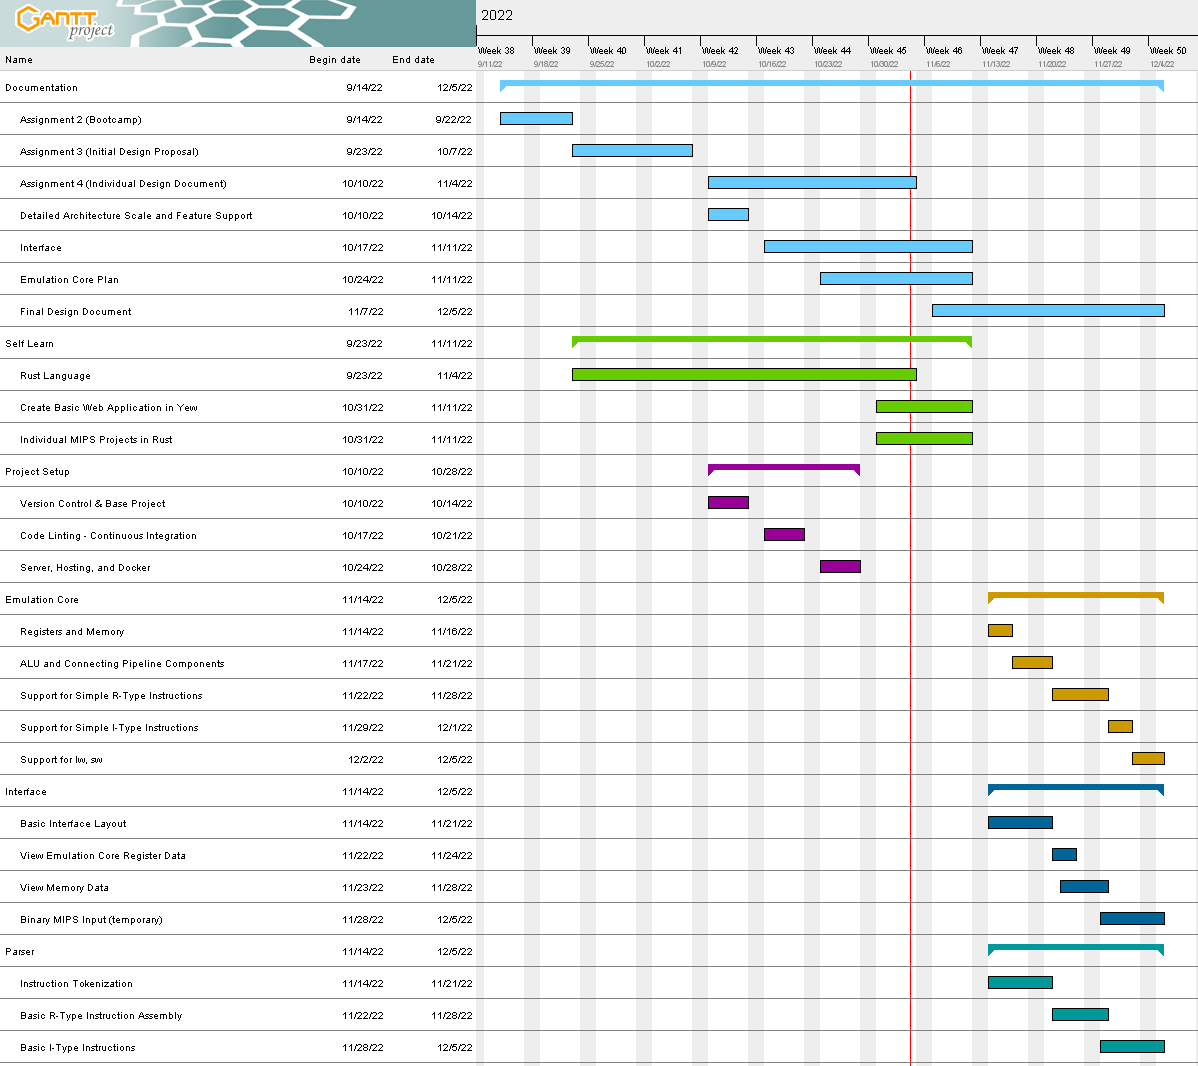
\includegraphics[width=\textwidth]{gantt-sd1}
    \caption{Senior Design 1 Gantt Chart (Updated 11/4/2022).}
\end{figure}

\begin{figure}[H]
    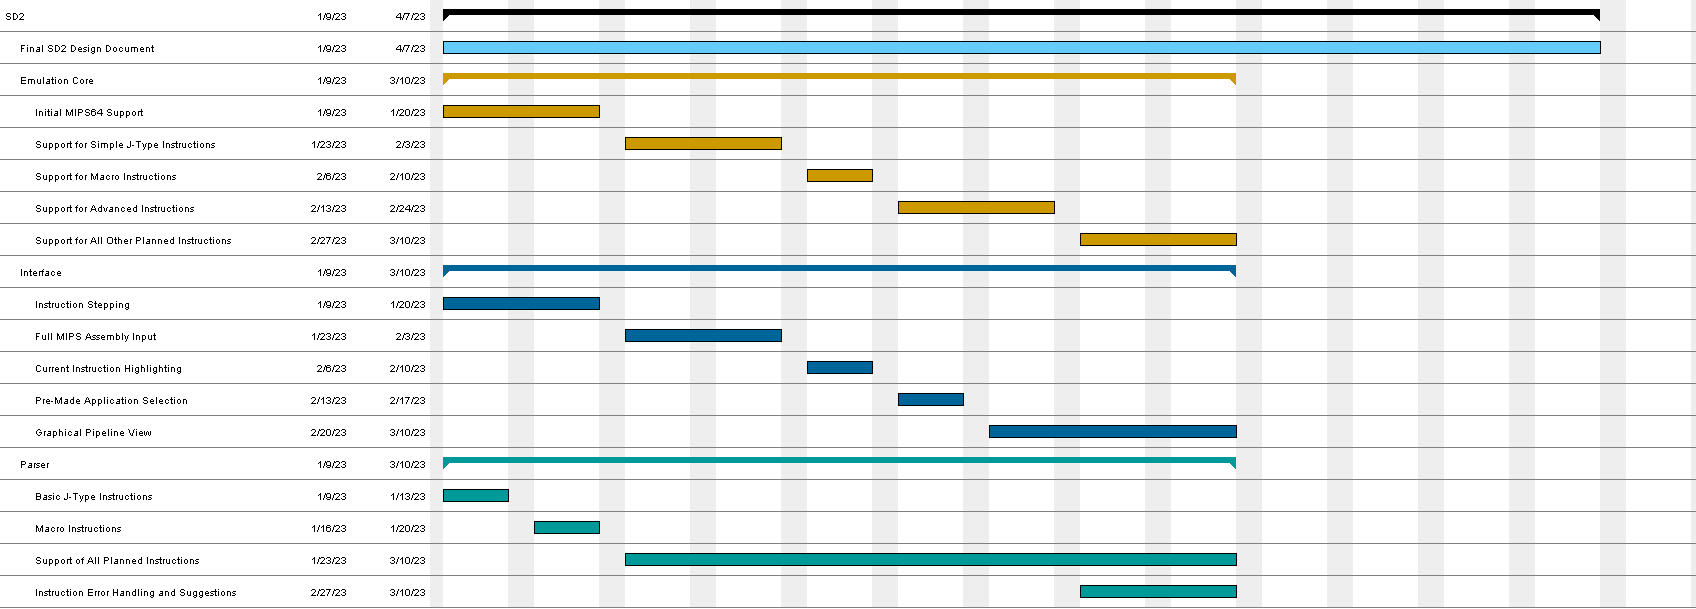
\includegraphics[width=\textwidth]{gantt-sd2}
    \caption{Senior Design 2 Gantt Chart.}
\end{figure}

\subsection{Asynchronous Communication}

During Senior Design 1, it became apparent with our group that
asynchronous communication and collaboration was crucial for the success
of the project. We determined early-on that our only synchronous meeting
time would be for an hour once a week, which is not enough for the
amount of work and scope needed for a Senior Design project such as
this. To circumvent these limitations, an emphasis was placed on the use
of tools or services that can facilitate this asynchronous
communication.

\subsubsection{Discord Bot}

One category of tools researched for this project is the use of a
Discord bot to allow daily Scrum-like standup meetings without the need
to meet synchronously, to keep all group members accountable and to keep
a continuous set of status updates with group members, should there be
no other communication. Many different bots were tested, each with their
own advantages and limitations. Discussed are a few of these bots and
reasons for and against using them.

The Orli Discord bot \cite{orli} was the most prominently advertised and
highest in search results for queries such as ``agile scrum discord
bot.'' This bot was, by first inspection, by far the most developed and
feature-rich, describing exactly what our group would have wished for in
a Discord bot. However, there were many issues found surrounding the
development and support for the bot that ultimately caused other bots to
be sought. One of these issues found immediately was the lack of an easy
way for anyone to activate the bot and invite it into a Discord server.
After gaining access to the bot, there were links to access setup
guides, however those links returned empty pages or error responses.
Furthermore, this bot was supposed to be able to integrate with GitHub
to connect project issues with tasks on Orli. Attempting to use this
functionality was met with more issues that had already been documented,
but not resolved after a few months. For these reasons, it was
determined that Orli would not be an effective Discord bot to facilitate
our group's asynchronous communication.

There were many unhosted open-source Discord bots available as well
\cite{austen-scrum-bot, navn-standup-bot, fijter-standup-bot,
    vivek-scrum-bot}, however these had not been updated for a number of
years and were determined to not be worth the additional time and
resources to run, as a reliable hosting solution to run a Discord bot
would have to be found, in a time period where the exact hosting
solution for the parent project, SWIM, had not yet been decided.

With these options considered as non-viable, DailyBot \cite{dailybot}
was the next solution found through research. While this Discord bot
does not have free and quick integration with GitHub, it was determined
that it could still act independently to a third-party service without a
significant overhead for using both services simultaneously. DailyBot,
in our primary use for it, prompts all group members daily for Scrum
questions via personal direct message on Discord. After filling out the
responses, the final result is sent to our shared Discord server for
other group members to view.

This bot was used for about 1 month during project development, however
we found that the limitations of the bot after the expiration of its
free standard plan trial made it unusable for our group. While this was
no longer used, we continued to send daily scrum information by simply
continuing to write in our Discord server, on the same schedule the
DailyBot provides us, and with the retrospective reports at the end of
the work week. It is at this point that we realized we may not need a
bot or a software to record and oversee our progress at all since at the
end of the day we are still doing this by ourselves. However, the
DailyBot does give good insight on how daily scrums are made, so that we
follow suit with a different method after it becomes less of a use to
the team.

\subsection{Version Control and Continuous Integration}
\label{subsec:version-control-and-ci}

Our group has decided to use GitHub as its primary location of storing
and collaborating on code for this project, due to its wide use in
open-source communities and familiarity from creating previous projects.
There are a few important considerations used when creating the process
to version control and create consistent, valid code. When publishing
any new code to the project, it should be the case that it has no
compilation errors, follows good coding practices, and passes all test
cases. To enforce this, both client-side and server-side checks are used
to keep all group members to a defined standard before code is added to
the main project.

On each cloned instance of the main git repository, a pre-commit hook is
brought with the project. We felt that this method of enforcing
client-side checking would be the simplest and most effective, as it
would be a built-in part of the ``git add, git commit, and git push''
cycle. However, this method of using git hooks is at first not automatic
and requires one manual step to be enabled due to a natural side effect
of how git repositories are structured. Usually, the default location
for git hooks in any given repository is .git/hooks, but hooks cannot be
distributed among group members in this directory since the .git folder
itself is a metadata folder that cannot be checked into version control.
To circumvent this, a makefile was added that can configure a local
instance of a git repository to use an alternative directory location
for git hooks. In the case of our project, the .githooks folder was
used. This allows our group to not only add a pre-commit hook with
automatic linting and testing, but leaves the hook open to be changed
later as seen fit. Any future changes to the hook or additional hooks
added later would be applied automatically when pulling the latest
remote changes.

Client-side formatting, linting, and testing is ideal for quick
revisions and local testing, but are easy to disable or otherwise avoid.
Server-side checking is also used in our project to ensure that all code
that will be merged into the repository's main branch passes all format
checking, linting, and tests. This can all be done with built-in
functionality from GitHub as part of their services, so this was the
method chosen to perform server-side checks.

The ideal, as previously stated, is that all code passes all checks and
tests before it is added to the main branch. To enforce this, all team
members are denied to push any changes directly to the main branch and
if this is attempted, the \texttt{git push} command will result in an
error. Instead, all changes must be first pushed to a branch, which can
then be added through a pull request on GitHub. This pull request can be
enforced to have certain checks pass before being merged into the main
branch. Checks are run remotely using GitHub Actions, which
automatically executes a series of commands on enabled triggers.

\begin{figure}[H]
    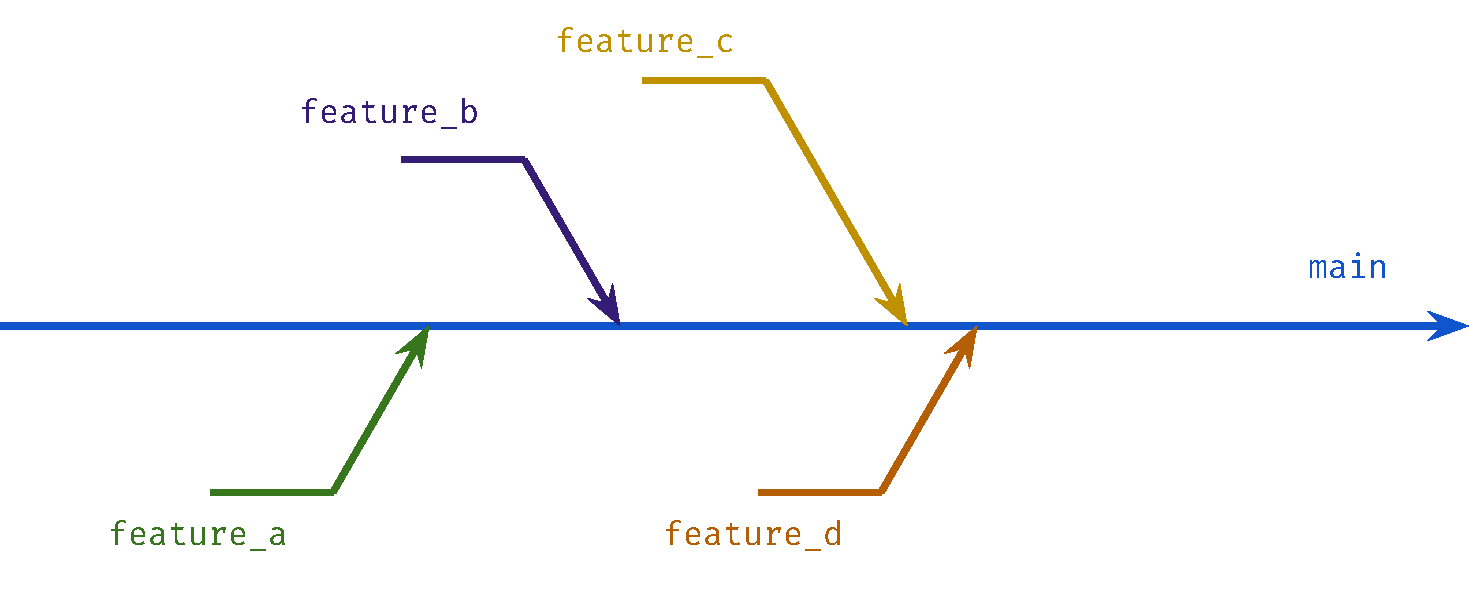
\includegraphics[width=12cm]{git-branching}
    \caption{Demonstration of all branches linearly added to the main branch.}
\end{figure}

To add a new feature to the main branch, a new change must first be
added to a separate branch and then have a pull request opened with it.
When pushing a new branch, GitHub will automatically suggest creating a
new pull request, making this process quick.

\begin{figure}[H]
    
\includegraphics[width=\textwidth]{github-pr-suggestion}
    \caption{GitHub's auto-suggestion to create a new pull request.}
\end{figure}

After creating the pull request, automatic checks are run using GitHub
Actions, until checks pass.

\begin{figure}[H]
    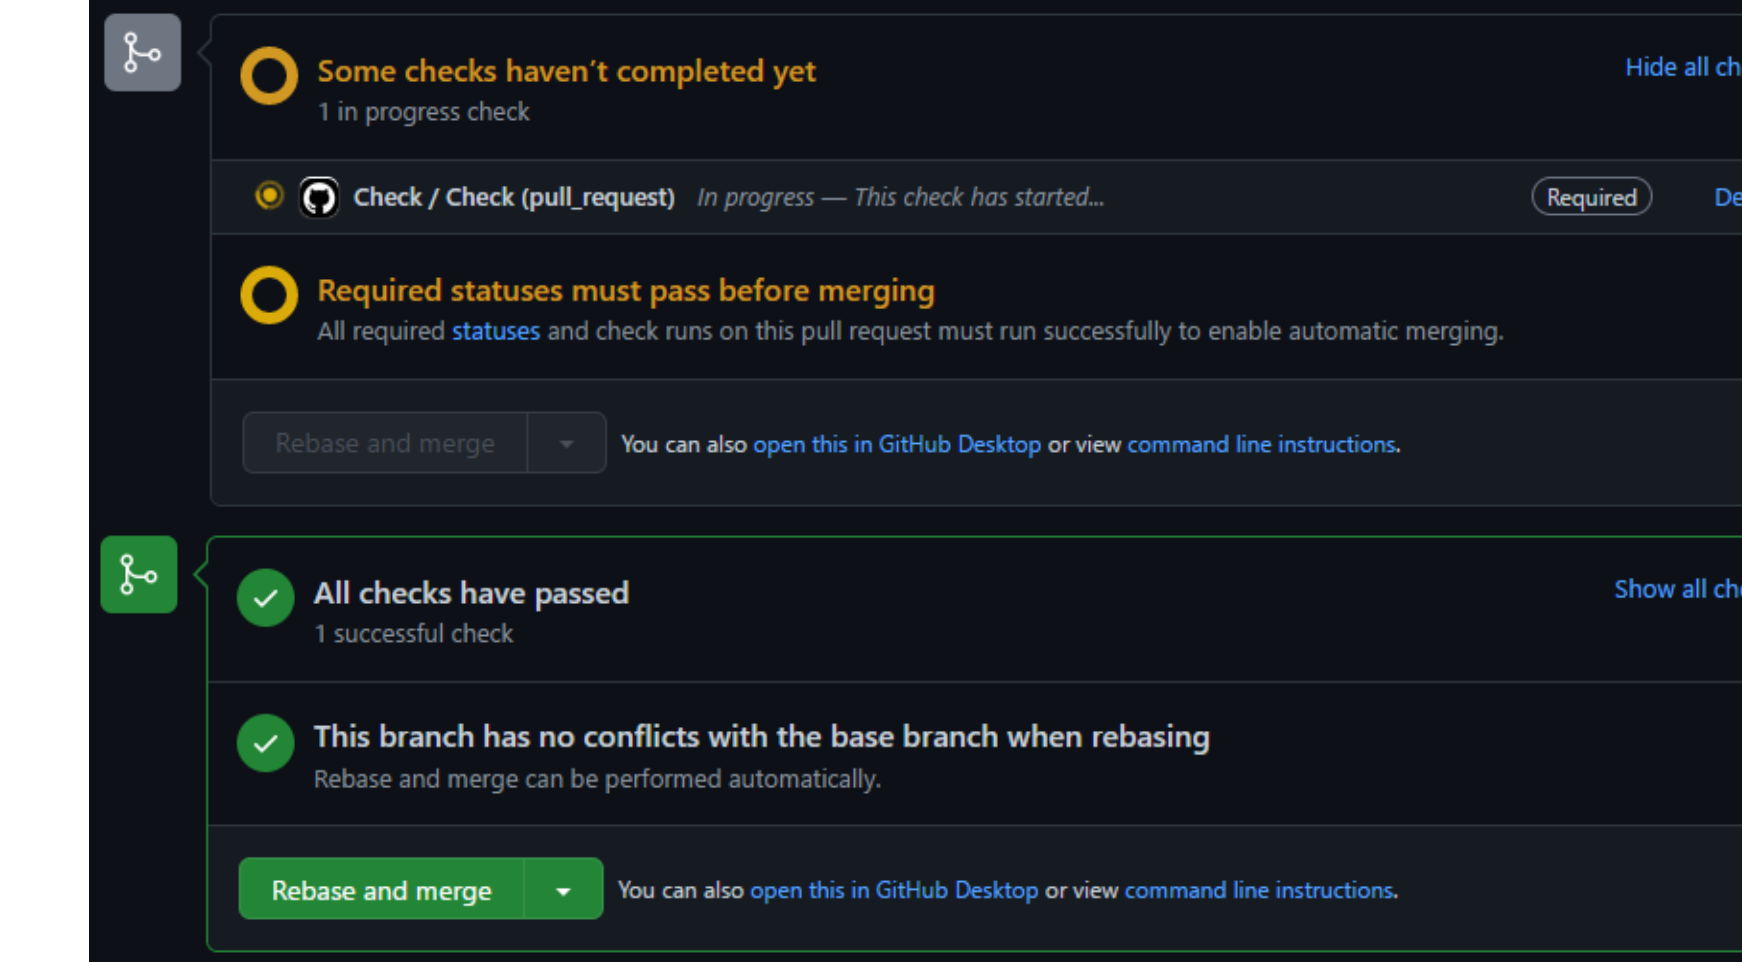
\includegraphics[width=12cm]{github-actions-testing}
    \caption{Testing results during testing and after passing.}
\end{figure}

The additional requirement has been added that not only does a branch
from a pull request pass all tests, but it must also be up-to-date with
the main branch. This avoids any possibly conflicting changes that occur
when merging. Instead, the main branch can be merged into the working
branch for a given feature, then all changes are rebased linearly onto
the main branch.

\begin{figure}[H]
    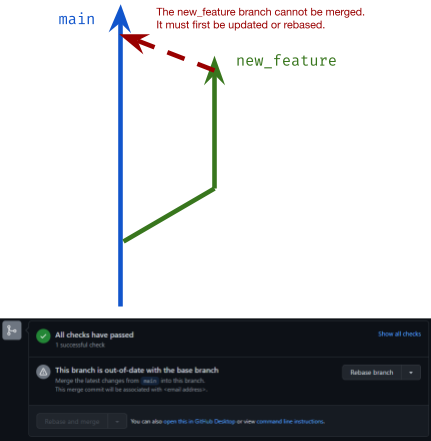
\includegraphics[width=12cm]{github-no-merges}
    \caption{Demonstrating the restriction of no merges and to be up-to-date with the main branch.}
\end{figure}

\subsection{Deployment}
\label{subsec:deployment}

Our project is deployed using GitHub Actions onto GitHub Pages due to
its easy integration and support with an existing repository hosted on
GitHub, especially one that is already using GitHub Actions for testing.
Additionally, this solution incurs no charge for us, making it an
incredibly compelling option. While GitHub Pages is not capable of
delivering dynamic pages, static resources and pages are easily
deployable. Since trunk outputs the project build into a single folder
of static HTML, CSS, JS, and WASM files, we feel that GitHub Pages is
well-suited for this project.

\begin{figure}[H]
    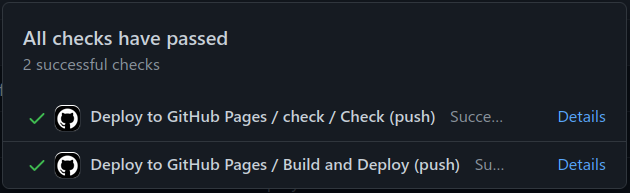
\includegraphics[width=\textwidth]{github-check-status}
    \caption{Example of GitHub showing the status of checking and deployment.}
\end{figure}

The repository is configured \cite{actions-gh-pages} to automatically
test, build, and deploy the project each time the main branch has new
changes, with the average time from merging to deployment taking less
than 5 minutes, which we consider to be effective for the project. While
setting up deployment, we found a number of changes that had to be made
with GitHub Actions to allow it to operate properly. The existing GitHub
Actions workflow responsible for checking the code for errors should
ideally be utilized and passed before proceeding ahead to deployment. By
default, workflows cannot be triggered by other workflows, so we had to
add the \texttt{workflow\_call} trigger to the existing check action,
which then allows a deployment workflow to call this first.

Additionally, specific to Yew and trunk, GitHub Pages did not initially
work properly in deployment. Since GitHub Pages formats the URL of the
page to be ``\textless repository owner\textgreater.github.io/\textless
repository name\textgreater,'' the fact that the page is not located at
a base domain name causes issues with Yew and its routing
\cite{stackoverflow-yew-github-actions}. To resolve this, we pass the
repository name into the \texttt{-\/-public-url} option of \texttt{trunk
    serve} within the GitHub Actions deployment workflow. To make this
change generalized to any repository, it was set to pull the name of the
repository and use this automatically for the \texttt{-\/-public-url}
option \cite{stackoverflow-github-actions-folder-name}. GitHub Pages is
configured predictably to the same URL structure in practice.
Admittedly, this does cause issues with repositories with the name
``\textless owner\textgreater.github.io'', as this creates an exception
with the page URL naming scheme used with GitHub Pages, but this is not
an issue for our repository in particular.

Outside of these changes, additional optimizations were implemented to
reduce the time the project takes to build during testing and
deployment. It is notable that GitHub Actions uses a random
pre-configured machine on GitHub's servers to run any scripts, meaning
that while the environment you receive on the start of a workflow is
consistent, changes are not saved by default. This implies that a new
build, either for testing or deployment, is from scratch each time. A
project with Yew can easily take over 15 minutes for an initial build,
making revision and collaboration slower. A number of changes were made
to compensate for this machine configuration.

First, instead of installing clippy (for testing) from \texttt{cargo
    install clippy} each time the workflow is run, this is instead brought
from a built-in GitHub Action \cite{ga-rust-toolchain} that installs a
pre-configured Rust toolchain, that includes clippy, rustfmt, and cargo.
For installing \texttt{trunk}, this is provided with a separate workflow
\cite{ga-trunk} that provides a pre-compiled binary instead of compiling
it each time. While these are great improvements to the time it takes to
test and deploy, these steps do not affect the build time of the project
itself. To accommodate this, we first optimized the testing process to
use the \texttt{-\/-no-deps} options in clippy. This avoids running
tests for dependencies of the project, which is desired, since these
dependencies are abstracted out of context for the sake of this project.

Additionally, a final pre-made workflow \cite{ga-rust-cache} was added
that implements caching for builds on GitHub Actions. While this can be
done manually as a feature within Actions, this workflow is configured
to automatically cache files and directories commonly cached in Rust
projects. Since the project itself will be the only major Rust crate to
change each time it is built, this makes the build significantly more
efficient. In initial testing, we have found that with these
optimizations and changes, the time to test and build was reduced from
about 10 minutes to less than 30 seconds.

One issue we have yet to see with this project is how GitHub Pages
handles redirection of subdirectories to the project. Since Yew apps are
single page applications, many URLs direct to the same one page, where
Yew then routes the user to the specified location. Since GitHub Pages
only offers static pages, redirection from these subdirectory URLs may
not be supported. While this may become a topic of discussion later,
this may also not be an issue if all our project operates on the primary
URL of deployment.

\section{Testing}

With SWIM, the goal is to not only create a functional product but to
also create a user experience that is as easy to work with as possible
with MIPS32 or MIPS64. To do this, we want to make sure that SWIM has as
few technical issues and bugs as possible and has an engaging and
pleasing interface. To that end, we are planning on not only having
extensive unit testing but are also planning on having a thorough user
experience test plan, as well.

% TODO: Edit this after SD2
From a broad perspective, there are three distinct sections to SWIM: the
emulation core, the parser, and the visual front end. While these
sections will all interface with each other in the end product, they
will largely be considered isolated systems for the sake of development.
Because of this, we will not be able to test interactivity between the
three sections until relatively later during Senior Design II. Not only
this, but many smaller aspects of the software might be used so
infrequently that, if there is something wrong, it may be unnoticed for
an extended period of time. To combat these potential issues, we are
planning on having extensive unit tests in place for automated testing.
That way, we are able to automatically test systems and ensure that
layering the systems on top of each other does not cause any unexpected
issues somewhere else in the project.

To that end, no section or subsection of the project will be considered
finished until there are extensive unit tests in place that can be run
automatically whenever anything is changed in the project. The plan is
to have multiple unit tests for each piece of code that are able to test
the function or file through a variety of use cases, so we are able to
have a reasonable level of certainty that all use cases have a unit test
to ensure that the software is operating as it was intended to. Of
course, any addition or modification to the project cannot be added to
the main GitHub repository until it has successfully passed all of the
unit tests built for that file or function itself. Then, the unit tests
for all of the other parts of the project should be run. Once all of
these unit tests have passed, we should know with certainty that the
software additions that we are adding to the project will not be
breaking any other piece of the project. For more details on the
automatic testing process in place, see Section
\ref{subsec:version-control-and-ci}.

The main important focus of our unit testing is going to be on the
emulation core, as it is both a core component of the project and issues
for niche cases can easily be undetectable in development. To this end,
each instruction written needs at least one unit test, or multiple for
more complex instructions.

Anecdotally, the merit of testing is clear. Project member Kevin Cahalan
worked on an emulator written in Rust for an internship, and the process
for developing this was test-driven. Instruction tests were written
before program code, which in effect was a way of documenting what the
instructions were intended to do. The tests additionally help with
learning and understanding the codebase. Everything had a test, not just
the emulation core.

The Rust toolchain comes pre-equipped with support for testing, making
this goal for extensive unit testing easy and effective in development.
Using the command \texttt{cargo test}, a suite of tests can be run,
disabled, or enabled per the needs of development. As an example of the
simplicity of Rust's testing facilities, Figure
\ref{fig:testing-registers-example} demonstrates tests for accessing
emulation core registers.

\begin{figure}[H]
    \begin{Verbatim}[frame=single, framesep=2mm, label=src/tests/emulation\_core/registers.rs]
use crate::emulation_core::mips::registers::{RegisterType, Registers};

#[test]
fn access_valid_register_by_enum() {
    let mut registers = Registers::default();

    registers[RegisterType::T2] = 4;

    assert_eq!(registers.gpr[10], 4);
}

#[test]
#[should_panic]
fn access_bad_register_by_string() {
    let mut registers = Registers::default();

    registers["not_a_real_register"] = 7;
}
    \end{Verbatim}
    \caption{Example of testing in Rust.}
    \label{fig:testing-registers-example}
\end{figure}

% TODO: Consider writing about meeting a code coverage quota using tarpaulin (https://github.com/xd009642/tarpaulin)

% TODO: Add information on testing the front end

\section{Browser Support}
\label{sec:browser-support}

The central idea of SWIM is to make working with MIPS32 and MIPS64 as
easy as possible. To that end, SWIM is a browser-based emulator,
eliminating the need for the user to download any software to use our
project. From a design perspective, this decision also eliminates
considering operating system support. However, our project working in
one web browser does not guarantee support in others. An important task
is to determine which browsers should be supported, and consequently
that all technologies in the project are compatible with all of those
browsers. Our group focused on ensuring compatibility with the most
frequently used web browsers.

\begin{figure}[H]
    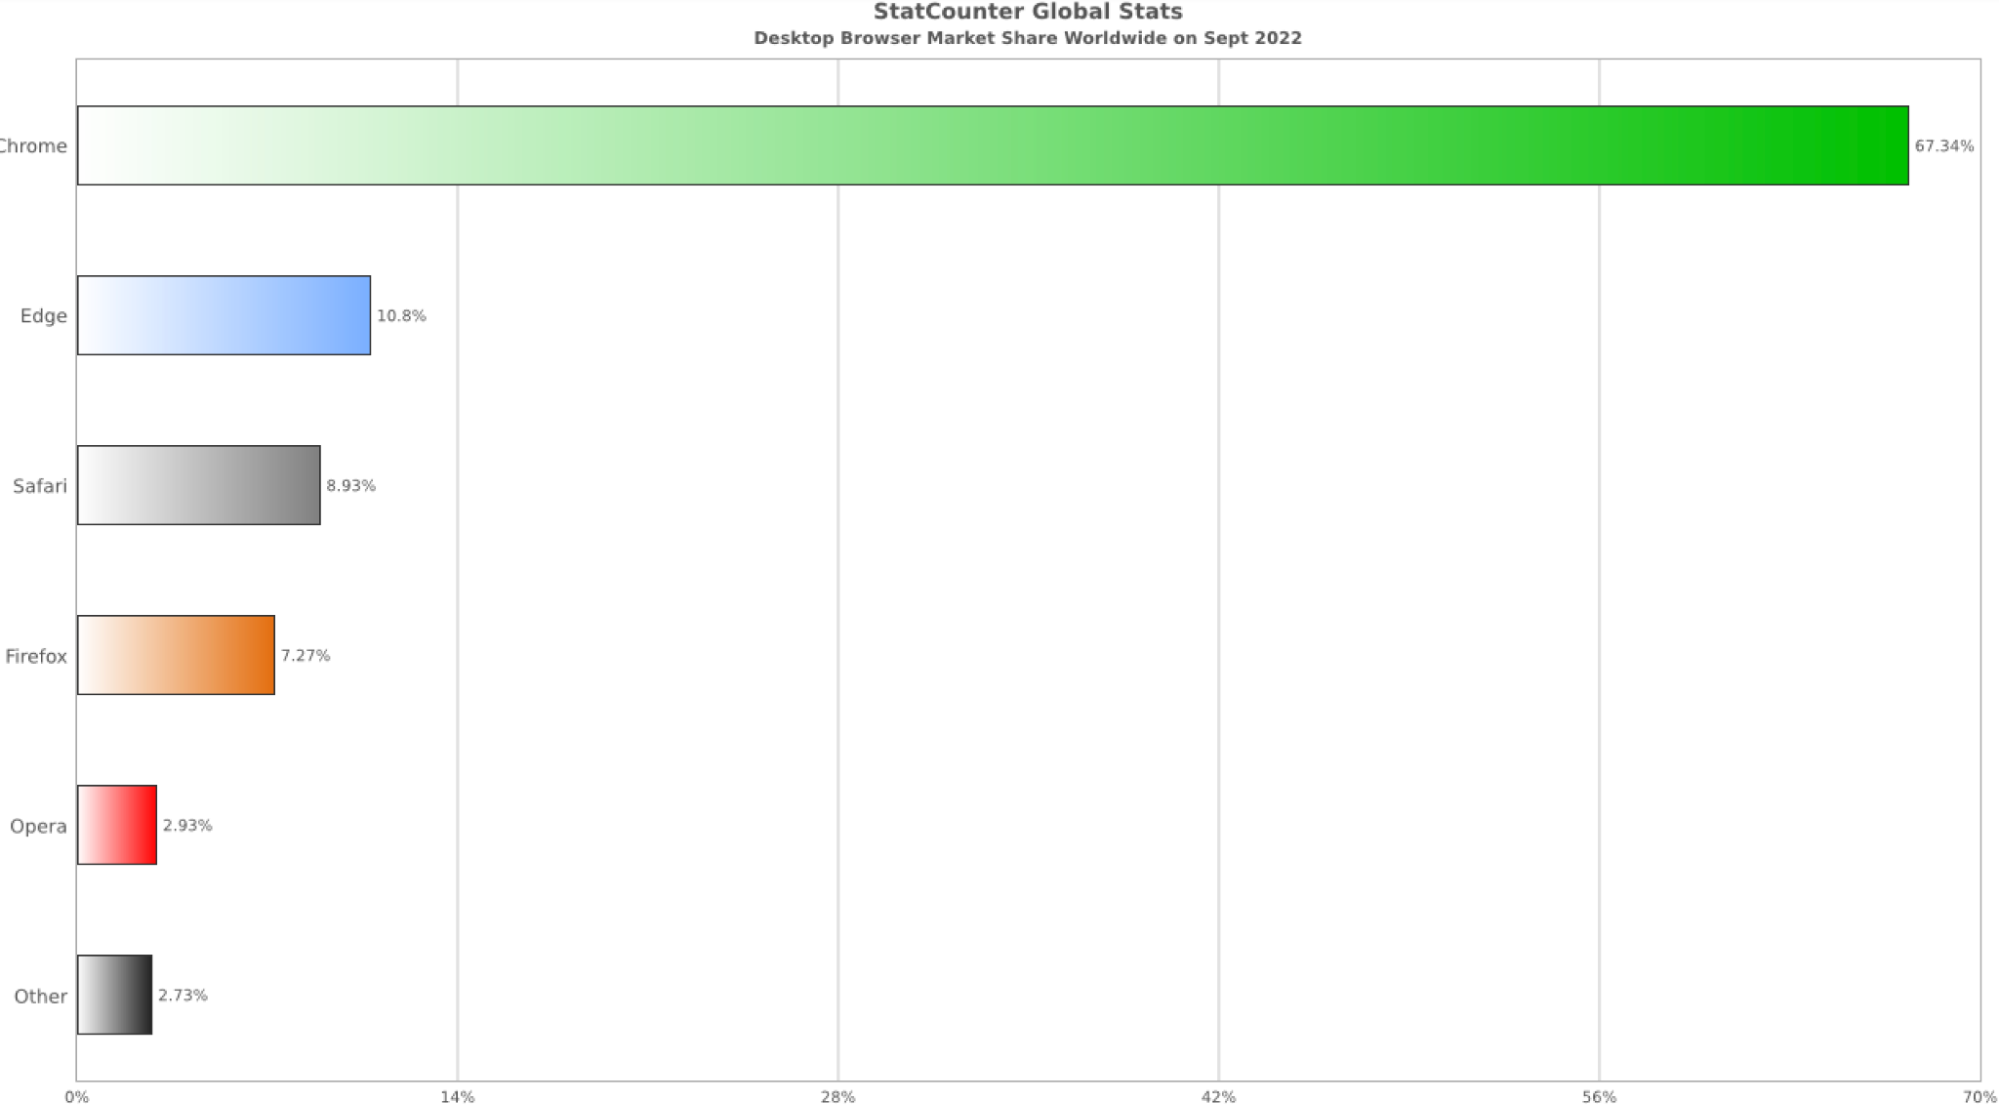
\includegraphics[width=\textwidth]{browser-global-stats}
    \caption{Desktop Browser Market Share according to \protect\cite{statcounter}. Used with
        permission.}
\end{figure}

According to \cite{statcounter}, the most commonly used browser on
desktops worldwide as of September of 2022 was Google Chrome with over
two-thirds of the market share. The top four most-used web browsers on
desktop -- Google Chrome, Microsoft Edge, Safari by Apple, and Mozilla
Firefox -- account for over 94 percent of the global web browser market
share on desktop. Because of this, we want to guarantee that our project
is fully functional on these four browsers at a minimum. Google Chrome,
Microsoft Edge, Opera (the fifth most-used browser), and Brave, are all
based on the open-source project Chromium, and compatibility for one
generally implies compatibility for the others. This resulted in a
slightly reduced workload when testing.

For the four browsers, our first goal was to ensure that the various
technologies used for the project are all fully supported. The first
technology we checked on for this was the main programming language we
are going to be building our project in, Rust, or by extension, the
language it compiles to, WebAssembly. WebAssembly has support for
Chrome, Edge, Safari, and Firefox on desktops and laptops according to
\cite{mdn-webassembly}, one of the main developers of WebAssembly, and
with this compatibility list, Opera is listed as having full support,
too.

Another major technology we needed to make sure is fully compatible with
all of the browsers we want to support was Monaco \cite{monaco}, the
code editor library our users use to write their MIPS64 programs.
According to its developer, Microsoft, the Monaco Editor has support for
Chrome, Edge, Safari, and Firefox. It also mentions support for the
Opera browser.

As shown on Figure \ref{fig:browser-technology-support}, all of the
browsers we were planning on supporting are compatible with the
aforementioned technologies. This meant that our project has not run
into any compatibility issues.

\begin{figure}[H]
    {\renewcommand{\arraystretch}{1.4}
        \begin{tabularx}{\textwidth}{|c|cccccc|}
            \hline
                                     & \multicolumn{6}{c|}{\textbf{Support for Technology By the Browser}}                                                                                        \\\hline
            \textbf{Technology}      & \textbf{Chrome}                                                     & \textbf{Edge} & \textbf{Safari} & \textbf{Firefox} & \textbf{Opera} & \textbf{Brave} \\\hline
            Rust through WebAssembly & \checkmark                                                          & \checkmark    & \checkmark      & \checkmark       & \checkmark     & ?              \\\hline
            Monaco Code Editor       & \checkmark                                                          & \checkmark    & \checkmark      & \checkmark       & \checkmark     & ?              \\\hline
            JavaScript               & \checkmark                                                          & \checkmark    & \checkmark      & \checkmark       & \checkmark     & \checkmark     \\\hline
        \end{tabularx}}

    \vspace{\baselineskip}

    \checkmark : Has support\\
    $\oslash$ : Does not have support\\
    ? : Support is not specified

    \caption{Support for browser technologies.}
    \label{fig:browser-technology-support}
\end{figure}

\section{Naming Our Project}
\label{sec:naming}

One unique issue we had with our project was coming up with a name for
it. The original pitched name for the project was OurSPIM, as SPIM is a
popular emulator for MIPS that inspired Kevin Cahalan, to originally
pitch this project. However, this project is not affiliated with the
team who created SPIM, and using SPIM in the name of the project may
incite unforeseen legal or ethical issues.

Below is a list of some of the other names that were considered during
the development of the project:

\begin{itemize}
    \tightlist
    \item OurSPIM - Derived from a UCF CDA3103 homework assignment name
          ``mySPIM.''
    \item SOME - Simple Online MIPS Emulator
    \item MISO - MIPS Intuitive System Online
    \item SWIM - Simple / Streamlined Web Interface for MIPS
    \item BEMP - Browser-based Emulator for the MIPS Processors
    \item MOE - MIPS Online Emulator
    \item MORE - MIPS Online Rust Emulator
    \item ucfSPIM - SPIM for UCF
    \item NeoSPIM - New Simple Online MIPS Emulator
    \item Generic\_Senior\_Design\_Project\_1234
    \item MIPandNayNay64 - A name suggested in jest based on the 2015 song
          \emph{Watch Me} by Silent\'o.
\end{itemize}

A consideration with naming our project are any possible restrictions
with a specific name. For example, if our project supports MIPS
initially and uses a MIPS-centric name, but later adds support for
RISC-V, the name may no longer hold relevance. Any later changes in the
project name would affect project discovery and could be difficult to
find after.

Another issue with naming our project in the same vein is if the name of
the project is too generic or too complex. In either case, this makes it
more difficult to find using common search engines. In an example of
being too generic, using a name like ``MISO'' could cause web searches
to return results around miso soup. The names ``SWIM,'' ``SOME,''
``MORE,'' and ``MOE'' all have similar issues. In being too complex, a
user may never remember the name or it could be difficult to type
quickly.

Using commonly recognized words and acronyms may help with naming and
recognition, for example in the name ``ucfSPIM.'' This is a memorable
and solid project name as it is made by UCF students, however for the
same reason as OurSPIM, there are possible legal implications that
cannot be foreseen.

With these considerations, the compromise was ultimately made to name
the project ``SWIM'' for its simplicity and lack of legal and ethical
issues. While another name may more appropriately satisfy the previous
considerations, no best name was found during the time of development.

\section{The Future of the Project}

The following subsections outline some of the future considerations for
project functionality not outlined otherwise. It is our goal to leave
SWIM as a long-standing project that other developers could contribute
to, should there be interest. This may involve a future Senior Design
team or the open-source community at large.

\subsection{RISC-V Support}

While MIPS has previously been used in landmark devices such as the
original Sony PlayStation and has become the de facto instruction set
architecture for studying computer logic and design, it is aging in
comparison to modern architectures. Both the team working on MIPS and
the 6th edition of Hennessy and Patterson's textbook have moved to
discussing RISC-V rather than MIPS \cites[p.~xviii]
{hennessy-patterson-6}{mips-to-risc-v}. MIPS could be considered by this
to be falling out of favor, and so to continue to maintain relevance in
education, should support RISC-V. There is a great chance that the
majority of students learning computer architecture in a decade will
have introduced to RISC-V, or even another ISA altogether.

It should be noted that RISC-V appears to, in some regard, bear strong
resemblance to MIPS, as they are both RISC architectures. The emulation
core is written in a way that another ISA could be supported easily, and
there may be similar portions of code that can translate to other
architectures. Additionally, the parser would not need to change
drastically, since the assembly formats of MIPS and RISC-V share strong
similarities.

\subsection{Operating System Development Support}

With the initial plan of SWIM, operating system development will simply
not be supported. Memory permissions, CPU state, BIOS, and other topics
beyond the scope of the project are not considered for the sake of
development simplicity. Should any system calls be supported at the
current architecture, an operating system would likely be ``faked'' with
Rust and JavaScript. Supporting a custom operating system would greatly
improve the diversity of use for SWIM, and allow for professors of
operating system courses to suggest SWIM to their students.

% TODO: \subsection{A syscall API to allow for GUI and game development}

\subsection{Desktop Application}

Making a desktop application of SWIM may be a great feature to add, as a
web application depends on a constant internet connection. In addition,
for SWIM to exist as a web application, it must be continuously
available on a server, which may prove difficult in the long-term
without proper funding. A desktop application may be of interest for
future developers for the sake of accessibility. In implementation, it
may be possible to convert the web application to a local desktop
application relatively quickly using Electron.

\subsection{Mobile Support}

With the globally-increasing use of mobile devices between students, it
may be of interest to add support for this in SWIM in a future release.
To implement this, the current limitations of the Monaco editor
(mentioned in Section \ref{sec:browser-support}) must be considered by
either using a different editing library or adapting Monaco to be
compatible with mobile browsers. This, with other user interface
altercations, may be all that is necessary to support mobile devices. In
a future iteration, porting to a native mobile application could then be
seen as feasible with maturation of Rust support for mobile devices.

\subsection{Multiple File Support}

The initial version of SWIM only supports working with a single assembly
file at a time. Having support for programs that are built using
multiple files may be beneficial to test larger assembly programs. This
functionality has not been researched, but it could be seen as valuable
if SWIM grows in functionality and scope.

Alternatively, ``multiple file support'' may be interpreted as allowing
multiple assembly programs to be open in in the interface
simultaneously. In this case, this may involve the addition of a tabbed
system of editors, selecting between the one that is loaded within the
emulation core.

\section{Summary and Conclusion}

In broad strokes, the goal of our project was to create a user-friendly
emulator for MIPS64 with a focus on usability in learning computer
architecture. Computer architecture can be such a difficult subject
already, the central goal of ours became making the toolset as
accessible and easy to use as possible while also emulating MIPS64 as
accurately as possible.

SWIM is an online emulator to make it as accessible as possible. Users
do not have to dedicate any hard drive space or wait through download
time to use SWIM; everything is handled through the browser. The website
itself is written with the Rust programming language and the tools that
allow it to run on the web are WebAssembly, yew, and gloo. Thanks to
WebAssembly, we were able to use a powerful language like Rust to build
our website meaning we do not have to sacrifice low-level power in
exchange for the portability provided by commonly used web development
languages like JavaScript. Embedded into the front end is a Monaco code
editor, providing our users with a familiar yet powerful tool to work
with.

Code written in the editor is passed into a custom-built parser and
assembler that will provide meaningful information about each line of
code back to the front end to display to the user and then provide the
binaries of each line of code to a custom-built emulation core where it
is run. This emulation core was built to emulate MIPS64 as accurately as
possible complete with a fully-realized visual datapath.

Now, at the end of Senior Design II, our work on this first iteration
SWIM is complete. The project is built from almost 25,000 lines of code
and contains over 400 tests to make sure it stays working properly. SWIM
supports over 60 real instructions, over 15 pseudo-instructions, labels,
and all major data types. It takes advantage of Monaco's feature set
with mouse-hover information, error underlining, and error-messages and
suggestions all surfaced within the custom-built parser \& assembler.
And it features a 5-stage visual datapath with step-by-step execution.

\printbibliography

\end{document}
